% Save as latexmk -pdf -jobname="Thesis - Detecting Open Source Library Usage and License Disclosure Gaps in Android APKs - Shayan Ghiaseddin" main.tex
\documentclass[12pt,a4paper]{report}
\usepackage[a4paper,left=3.5cm,right=2.5cm,top=2.5cm,bottom=2.5cm]{geometry}

\usepackage{graphicx}
\usepackage{xurl}
\usepackage{hyperref}
\hypersetup{hidelinks}
\usepackage[english]{babel}
\usepackage{csquotes}
\usepackage{longtable}
\usepackage{array}
\usepackage{amsmath}
\usepackage{csvsimple}
\usepackage[strings]{underscore}
\usepackage{microtype}
\setlength{\emergencystretch}{3em}
\usepackage[style=apa,backend=biber]{biblatex}
\DeclareLanguageMapping{english}{english-apa}
\addbibresource{references.bib}


\begin{document}

\begin{titlepage}
    \centering
    \vspace*{0.38\textheight}
    {\fontsize{24.88}{38}\selectfont\bfseries THESIS WORK\par}
    \vfill
    \begin{flushright}
    {\fontsize{20.74}{24}\selectfont\bfseries Shayan Ghiaseddin\par}
    {\fontsize{20.74}{24}\selectfont\bfseries 2026\par}
    \end{flushright}
\end{titlepage}

\begin{titlepage}
    \begin{flushleft}
    {\fontsize{17.28}{20}\selectfont\bfseries Corvinus University of Budapest\par}
    {\fontsize{17.28}{20}\selectfont\bfseries Institute of Data Analytics and Information Systems\par}
    \end{flushleft}

    \vspace*{0.20\textheight}
    \centering
    {\fontsize{24.88}{30}\selectfont\bfseries Detecting Open Source Library Usage and License Disclosure Gaps in Android APKs\par}

    \vfill
    \begin{flushright}
    {\fontsize{17.28}{20}\selectfont\bfseries Shayan Ghiaseddin\par}
    {\fontsize{17.28}{20}\selectfont\bfseries Business Informatics MSc Programme\par}
    {\fontsize{17.28}{20}\selectfont\bfseries 2026\par}
    \vspace{1.2cm}
    {\fontsize{17.28}{20}\selectfont\bfseries Thesis Supervisor: Dr. Johannes Wachs\par}
    {\fontsize{17.28}{20}\selectfont\bfseries Associate Professor\par}
    \end{flushright}
\end{titlepage}

\tableofcontents

\listoffigures
% \addcontentsline{toc}{chapter}{List of Figures}
\listoftables
% \addcontentsline{toc}{chapter}{List of Tables}

\chapter*{Summary}
\addcontentsline{toc}{chapter}{Summary}

Modern Android applications are built from many external open-source libraries. These libraries help developers build apps faster, but they also create a visibility problem: users, auditors, and sometimes even developers may not know which third-party components are actually embedded inside an app. This matters because external libraries can contain vulnerabilities, become unmaintained, or create license obligations. If a library is used but not declared, its risk is difficult to notice and manage.

This thesis addresses that problem by developing an automated pipeline for detecting open-source library usage in compiled Android APK files. The pipeline collects APKs, decodes them, extracts license information, builds fingerprints from public source-code repositories, and matches those fingerprints against decoded application code. This makes it possible to compare what an application declares in its license information with what is actually detected in the code.

The final analysis is based on a corpus of 699 Android APKs from sensitive categories such as finance, health, communication, and navigation. The results show that Android applications rely heavily on external libraries, with an average of 154.84 detected library occurrences per APK. However, 44.61\% of detected library occurrences were not cited in license declarations. The fingerprint-based method proved effective, confirming most library usage through code evidence and revealing dependencies that license information alone would miss.

Overall, the thesis shows that the main risk is not simply the use of open-source libraries, but the gap between actual library usage and visible disclosure. The proposed pipeline provides a practical way to measure this gap and supports better dependency transparency in Android applications. In practical use, the pipeline can analyze a given APK and report which open-source libraries it contains and how healthy those libraries appear to be.

\chapter{Introduction}
\section{Problem Statement}
Modern software development heavily relies on open source libraries and external dependencies. Android applications are no exception, often incorporating numerous third-party components whose presence is not always documented in a standardized way. Most of the times, the original source code of mobile applications is not publicly available; for Android applications, researchers usually have access only to compiled APK files. This makes it difficult to determine which open source libraries are actually used by widely distributed consumer applications, and how deeply applications depend on external code.
Existing tools for detecting library usage inside APK files are limited. Therefore, there is a need for a scalable method to extract, identify, and analyze open source software references from Android applications and report potential risks.

\section{Research Objectives and Scope}
In this thesis, the terms \emph{external libraries}, \emph{open source libraries}, \emph{open source software (OSS)}, and \emph{libraries} refer to reusable third-party software components included in an Android application to provide specific functionality.

The objective of this thesis is to develop an automated and scalable pipeline capable of extracting references to open source libraries from Android APK files. The research aims to build a dataset of commonly used applications, detect declared and undeclared library dependencies, and analyze the extent of these dependencies. Another goal is to evaluate how reliably library usage can be identified through license declarations, package fingerprints, and repository metadata, and to assess the feasibility of large-scale dependency analysis in mobile applications. The thesis also aims to identify applications with the highest intensity of uncited unhealthy open source library usage.

The study is limited to Android APK files and does not cover iOS applications or other mobile platforms. It also does not validate decoded APK evidence against the original application source code, because that source code is generally unavailable. Finally, the thesis does not audit applications at runtime; library usage is evaluated through static evidence extracted from decoded APKs.

\section{Research Questions}
The research is guided by the following questions:
\begin{itemize}
\item (RQ1) Is it feasible to detect external libraries in Android APK files?
\item (RQ2) How reliable are license declarations and package fingerprints for identifying library dependencies?
\item (RQ3) How many open source libraries, and what types of them, are used in a sample of Android applications?
\item (RQ4) Which Android applications show the highest dependency on low-health or medium-health open-source libraries?
\end{itemize}

\section{Structure of the Thesis}
We first review open-source dependency risks in Android software, focusing on prior work about Android third-party library detection, software supply-chain security, and open-source license management. We then move to the pipeline I developed to collect APKs, extract library evidence, and build the dataset. Finally, the generated dataset is analyzed to compare detected library usage with license disclosure and to identify applications with higher uncited unhealthy-library exposure.

\section{Personal Motivation and Acknowledgements}
I chose this topic because I enjoy technical challenges. Detecting dependencies from the source code of Android applications would be relatively straightforward, but APK files are compiled final products where the original project structure is no longer directly visible. This makes dependency detection more difficult and makes the problem more interesting from both a technical and research perspective.

I would like to thank my supervisor, Dr. Johannes Wachs, for involving me in this research topic and for his guidance, support, and enthusiasm throughout the work.

Also, I would like to thank my wife, Shahrzad to support me in this journey.

\chapter{Theoretical Background}
\section{Modern Software Development and Dependency Ecosystem}

Modern software development has evolved from monolithic, self-contained programs toward highly modular systems built from reusable components, libraries, and services developed by third parties. This shift has been driven by increasing software complexity, economic pressure to improve productivity, and the emergence of collaborative development ecosystems.

In the early decades of computing, software was typically written as monolithic programs tailored for specific hardware systems. Programs were often developed from scratch, with little separation between components, and reuse was limited to informal sharing among research institutions and user groups \parencite{ojhaEmergenceOrganizationalField2014}. As software systems grew larger in the 1960s, developers encountered what became known as the \emph{software crisis}, characterized by cost overruns, unreliable systems, and difficulty managing complexity. The 1968 NATO Software Engineering Conference highlighted the need for disciplined engineering practices and emphasized modular design as a way to divide large problems into smaller, manageable units \parencite{randellSoftwareEngineering19681979}.

During the same period, the idea of systematic software reuse emerged. McIlroy proposed that software could be assembled from standardized modules rather than built entirely from scratch, introducing the concept of catalogs of reusable components. In parallel, early \emph{software factory} concepts suggested that development should follow standardized processes, reusable parts, and controlled environments to improve productivity and quality. This terminology became especially influential in Japan during the mid-1970s and 1980s, where software production was increasingly compared with industrial manufacturing \parencite{cusumanoSoftwareFactoryHistorical1989}. These ideas reflected the growing recognition that modularity was not only a technical choice but also an economic necessity.

In the 1970s, structured programming and principles such as \emph{coupling and cohesion} formalized the concept of modular design. High-level programming languages and improved compiler technology enabled independent modules to be developed and combined into larger systems, supporting parallel development and easier maintenance \parencite{newmanMonolithMicroservicesEvolutionary2019}. At the same time, software began to be treated as a commercial product rather than an inseparable part of hardware, further encouraging the creation of reusable libraries and third-party components.

The 1980s marked an important milestone with the rise of the \emph{free software} movement, later knowned as open source software. Projects such as GNU promoted the idea that software should be freely shared, modified, and redistributed, supported by licenses designed to preserve openness. This created a growing pool of reusable tools, compilers, and libraries that developers could incorporate into their own systems \parencite{ojhaEmergenceOrganizationalField2014}. Object-oriented programming also became widespread during this period, encouraging encapsulation and reuse through class libraries and reusable frameworks \parencite{aguilaSoftwareEngineeringTimeline2020}.

In the 1990s, open-source development moved from a niche practice to a widely adopted model. Large collaborative projects such as Linux demonstrated that complex systems could be built from many independently developed modules contributed by distributed communities. The emergence of public code repositories and standardized open-source licenses made it easier for developers to discover, integrate, and reuse third-party libraries \parencite{ojhaEmergenceOrganizationalField2014}. Component-based development and reusable frameworks became common, further reinforcing the modular approach \parencite{aguilaSoftwareEngineeringTimeline2020}.

During the 2000s, open source became commercially mainstream. Organizations increasingly relied on external libraries instead of developing all functionality in-house, reducing development costs and accelerating delivery through improved collaboration platforms and mature licensing models. At the architectural level, service-oriented architecture extended modularity beyond source code by allowing systems to be composed of independent services communicating over networks \parencite{fitzgeraldTransformationOpenSource2006,aguilaSoftwareEngineeringTimeline2020}.

In the 2010s, \emph{microservices architecture} and \emph{cloud computing} accelerated the shift toward dependency-based development. Applications began to consist of many small, independently deployable components, often combined with third-party libraries and external services. Modern software projects frequently contain relatively little original code, acting instead as orchestration layers around large dependency graphs maintained by global developer communities \parencite{newmanMonolithMicroservicesEvolutionary2019,aguilaSoftwareEngineeringTimeline2020}.

As a result of this historical evolution, contemporary software development depends heavily on external libraries and open-source components. While this modular ecosystem enables rapid innovation, it also creates challenges related to dependency management, transparency, and security, especially when the exact set of third-party components used by an application is not clearly documented. These challenges motivate the need for methods capable of identifying and analyzing dependencies in softwares.

\section{Open Source Libraries and Their Benefits}

Open-source libraries are central to modern software development because they provide reusable functionality that can be inspected, modified, and improved collaboratively. Their main benefit is not only code availability, but also collective review: many developers and users can test, improve, and maintain the same components, which can support innovation, faster defect discovery, and software quality comparable to proprietary alternatives \parencite{oreillyLessonsOpensourceSoftware1999,weberPoliticalEconomyOpen2000}.

Another important benefit of using open-source libraries is cost efficiency and faster development. Instead of building all functionality internally, organizations can integrate proven components, share the cost of common infrastructure, and focus internal resources on competitive features. This reduces development time, lowers financial costs, and improves productivity through repeated reuse across projects \parencite{chesbroughMeasuringEconomicValue2023,ajilaEmpiricalStudyEffects2007,lernerEconomicsTechnologySharing2005}. At the industry level, the economic value of open-source software is substantial, as replacing open-source components with proprietary alternatives would require significantly higher investment and development effort \parencite{hoffmannValueOpenSource2024}.

Open-source libraries also support knowledge sharing across the software ecosystem. Because source code is available, improvements created for one project can be inspected, adapted, and reused by others, leading to faster diffusion of technical knowledge, professional learning, and reduced duplicated effort across organizations \parencite{chesbroughMeasuringEconomicValue2023,lernerSimpleEconomicsOpen2002}.

Because of these advantages, applications today are rarely developed entirely from scratch; instead, they are assembled from numerous external components maintained by global communities. While this approach enables rapid development and innovation, it also increases the complexity of dependency relationships.

\section{Dependency Networks in Modern Software Systems}
Modern software development has become heavily reliant on open-source libraries and modules, creating extensive dependency networks that span entire ecosystems. 
A 2021 audit of over 947 commercial codebases found that 98\% contained open-source libraries \parencite{OpenSourceSecurity2026}. 
Each application-level dependency can itself have further requirements, forming a direct and transitive dependency graph. In other words, \emph{software supply chains} now consist of layers of upstream libraries and their downstream dependents, interwoven networks of packages maintained by vast communities.

In an open-source dependency network, developers declare direct dependencies on certain library packages, and each of those libraries may bring in its own dependencies (transitive dependencies). Package managers, as development tools, automatically resolve and fetch this full transitive closure of the dependency graph to build the project \parencite{boldiFineGrainedNetworkAnalysis2020}. As a result, a project that directly uses only a handful of libraries might end up including dozens or hundreds of indirect libraries through recursive dependency chains. This deep nesting of components means that modern applications implicitly trust not only the libraries they explicitly import but also all the dependencies of those dependencies. The dependency graph thus often spans many levels, and managing it requires considering not just individual packages but the entire tree of interconnected software components.
Over time, these open-source dependency networks have grown immense in scale and depth. For example, the npm repository for Node.js now hosts over 5.5 million packages \parencite{LibrariesioSecurityMaintenance2026}, and other ecosystems (Maven, PyPI, RubyGems, etc.) have similarly exploded in size. The typical software project today relies on dozens of third-party libraries: according to a corporate report, the average number of open-source components per application was 1,180, and 64\% of open-source components in a typical codebase were transitive dependencies pulled in automatically by direct dependencies \parencite{OpenSourceSecurity2026}.

Critically, the dependency networks are not only large but also highly interconnected. \citeauthor{boldiFineGrainedNetworkAnalysis2020} (\citeyear{boldiFineGrainedNetworkAnalysis2020}) observe that ecosystems have become extremely fragile, with certain core libraries serving as hubs that many others rely on. In the RubyGems ecosystem, for instance, a single popular library was found to appear in the dependency trees of over 400,000 other packages – meaning that if this one library were removed, about 40\% of the entire ecosystem would cease to work \parencite{zeroualiImpactSecurityVulnerabilities2022a}. This example shows how a small change in a widely used component can have a cascading effect across countless applications. The overall number of issues scales with this growth as well: 
according to the \citeyear{OpenSourceSecurity2026} Black Duck OSSRA report, audited codebases contained an avarage of 581 total vulnerabilities but only 237 average unique vulnerabilities, showing that many vulnerabilities appear multiple times across the same application because of duplicated and repeated dependencies in complex dependency trees \parencite{OpenSourceSecurity2026}.

One prevalent problem arising in these sprawling networks is \emph{dependency bloat}. This refers to libraries that are included in a project’s dependency tree but are never actually used by the project at runtime. Bloated dependencies needlessly increase software footprint and can even introduce additional risk or maintenance work without any benefit. Empirical analysis of the Maven Central (Java) ecosystem shows that bloated dependencies are common and tend to persist over time: in one longitudinal study of 435 Java projects, the number of bloated (unused) dependencies steadily increased with each release, and fully 89\% of the dependencies identified as bloated in a given project version remained bloated in all subsequent versions of that project \parencite{soto-valeroComprehensiveStudyBloated2021}. In other words, once a library is added and turns out to be unnecessary, developers rarely remove it. In addition, \citeauthor{soto-valeroComprehensiveStudyBloated2021} (\citeyear{soto-valeroComprehensiveStudyBloated2021}) found that about 22\% of the dependency update operations performed by developers were devoted to updating these unused libraries. Such effort is essentially wasted, since those libraries did not need to be there in the first place. Dependency bloat shows how deep dependency networks can make the overall software stack heavier and more difficult to manage.

Another critical issue introduced by deep and complex dependency networks is the \emph{propagation of vulnerabilities} through the dependency tree. When a security flaw is discovered in a library, any application that directly or transitively depends on that library may be exposed to the vulnerability. As \citeauthor{boldiFineGrainedNetworkAnalysis2020} (\citeyear{boldiFineGrainedNetworkAnalysis2020}) point out, a bug or vulnerability in a single low-level library can affect a huge number of other libraries and applications that rely on it, whether directly or via transitive inclusion. \citeauthor{dusingAnalyzingDirectTransitive2022} (\citeyear{dusingAnalyzingDirectTransitive2022}) similarly report that vulnerabilities often influence downstream software through long chains of dependencies, such that a single vulnerable library version may end up impacting thousands of other artifacts that include it transitively. In effect, the dependency network acts as a wide distribution pipeline for exploits: a weakness in one component can radiate outward to many projects. 


Managing and mitigating these security risks has proven to be extremely challenging as dependency networks deepen. Developers and organizations frequently struggle to keep their dependencies up-to-date with the latest security patches. \citeauthor{dusingAnalyzingDirectTransitive2022} (\citeyear{dusingAnalyzingDirectTransitive2022}) note that, despite the availability of automated tools (such as dependency bots and vulnerability scanners), many developers find it difficult in practice to stay on top of upgrading vulnerable libraries. The result is that known vulnerabilities can linger in software for long periods before they are addressed. A comprehensive multi-language study by \citeauthor{kumarComprehensiveStudyImpact2024} (\citeyear{kumarComprehensiveStudyImpact2024}) observed that once a serious vulnerability is introduced via a dependency, it tends to persist for over a year on average in the affected projects before being fixed. This lengthy window of exposure underscores the slow adoption of security patches in dependency networks. Even when a fix has been released upstream, downstream projects do not always incorporate it promptly. Research on the npm and RubyGems ecosystems found that roughly 33\% of dependency vulnerabilities in GitHub projects could be resolved by simply upgrading to a newer patched version within the same major release of the library – yet those projects had not done so \parencite{zeroualiImpactSecurityVulnerabilities2022a}. When a new CVE (Common Vulnerabilities and Exposures) is announced in a popular library, maintainers of downstream projects must determine whether their software is impacted – a non-trivial task when the vulnerable code may be buried several layers deep in a transitive dependency. In summary, the deeper and more entangled the dependency network, the harder it becomes to monitor and manage security across all the included components.

\section{Security Incidents Caused by Vulnerable Dependencies}

Historical evidence shows that some of the most severe cybersecurity incidents of the last decade were caused by flaws in open‑source dependencies rather than in the application code itself \parencite{2026StateSoftware2026,pontaDetectionAssessmentMitigation2020}.
The Heartbleed vulnerability in 2014 affected OpenSSL, a cryptographic library used by a large share of web servers worldwide. A buffer over‑read flaw allowed attackers to access sensitive memory contents, including private keys and credentials, forcing emergency updates across millions of systems \parencite{2026StateSoftware2026}. In the same year, the Shellshock vulnerability in the GNU Bash shell enabled remote code execution on Unix‑based systems, demonstrating that even low‑level open‑source utilities can expose a large attack surface when they are widely deployed \parencite{2026StateSoftware2026}.

Dependency‑related incidents continued in later years. In 2017, attackers exploited an unpatched vulnerability in the Apache Struts web framework during the Equifax data breach, gaining access to the personal data of approximately 147 million individuals. The flaw had been publicly disclosed months earlier, but the affected systems were not updated in time, illustrating the risks of slow patch adoption in dependency networks \parencite{cordeySoftwareSupplyChain2023,2026StateSoftware2026}. The 2018 event-stream incident in the npm ecosystem demonstrated that malicious code could be inserted directly into a dependency. A compromised version of a widely used JavaScript package included hidden code designed to steal cryptocurrency wallet credentials, demonstrating that attacks may also originate from manipulated updates rather than accidental bugs \parencite{NpmBlogArchive2018}.

More recent incidents highlight the growing scale of the problem. Discovered in 2021, the Log4Shell vulnerability in the Apache Log4j logging library enabled remote code execution through specially crafted log messages and affected a vast number of enterprise and cloud applications. Because Log4j was included as a dependency in countless projects, organizations worldwide had to audit their systems to determine whether the vulnerable library was present, including cases where it was only included transitively \parencite{falconeAnotherApacheLog4j2021,pontaDetectionAssessmentMitigation2020}. In the JavaScript ecosystem, a severe prototype-pollution flaw in Lodash was found to potentially expose over 4 million GitHub projects through dependency graphs \parencite{liuDemystifyingVulnerabilityPropagation2022}. In 2022, the Spring4Shell vulnerability again showed how flaws in widely used frameworks can be exploited to deploy malware on servers that indirectly depend on the affected library \parencite{CVE202222965AnalyzingExploitation2022}.

A different type of dependency risk was demonstrated by the XZ Utils backdoor discovered in 2024. In this case, malicious code was intentionally introduced into the source of a widely used compression library by a contributor who had gained maintainer trust. Unlike ordinary vulnerabilities, this was not an accidental coding flaw but a deliberate supply-chain compromise that could have allowed remote access if it had reached stable releases \parencite{freireUnderstandingRedHats}. This incident emphasized the difficulty of securing open-source ecosystems where many projects depend on code maintained by external contributors.

Available statistics indicate that dependency-related security problems are increasing over time. CVE disclosures show a strong upward trend: reported vulnerabilities grew by 463\% between 2013 and 2023, and by the first half of 2025 more than 21,500 CVEs had already been disclosed, roughly 133 per day, with about 38\% rated high or critical. Malicious package activity has also accelerated: Sonatype reported 704,102 malicious open-source packages discovered since 2019, including more than 512,000 new malicious packages since November 2023, a 156\% year-over-year increase \parencite{OpenSourceMalware2025,VulnerabilitiesStatistics20252025}. These figures show why identifying the libraries embedded in compiled Android APK files is important: dependency risks can propagate widely, and their impact becomes especially serious in sectors where software handles sensitive data, regulated processes, or critical services.

\chapter{Industry Relevance and Sensitive Sectors}

\section{Why Industry Context Matters}
The risks created by external libraries are not distributed evenly across all software domains. Their impact depends on the sensitivity of the data processed, regulatory oversight, third-party integrations, and the organization’s ability to monitor dependencies over time. Although open-source usage is now nearly universal in commercial software, some sectors face stronger pressure because they combine deep dependency trees, strict compliance requirements, many interconnected applications, and serious consequences in the event of failure. In these sectors, incomplete visibility into external components can create operational, legal, and security risks that are more serious than in less regulated domains \parencite{OpenSourceSecurity2026,2024StateOpen2024,2026StateSoftware2026}.

\section{Financial Services}
Financial services are one of the most clearly sensitive sectors for dependence on external libraries. According to the 2026 OSSRA report, Financial Services and FinTech codebases show very high concentrations of high-risk vulnerabilities, reaching 92\%, while the same report also lists this sector among the industries with the highest license-conflict rates at 72\% \parencite{OpenSourceSecurity2026}. This pattern is linked to large and complex codebases, many integration points, and regulatory requirements that can slow updates and remediation \parencite{OpenSourceSecurity2026}. From a governance perspective, Sonatype notes that regulated industries, especially financial services, are early adopters of Software Bills of Materials (SBOMs), while the Digital Operational Resilience Act (DORA) requires financial institutions and ICT providers to strengthen oversight of software supply-chain risk \parencite{2026StateSoftware2026}. Therefore, external libraries in financial software are not only a technical dependency issue, but also part of compliance and audit responsibility \parencite{OpenSourceSecurity2026,2026StateSoftware2026}.

\section{Healthcare and Health Technology}
Healthcare, health technology, and life sciences also stand out as highly sensitive sectors. In the OSSRA industry breakdown, Healthcare, Health Tech, and Life Sciences codebases show high levels of serious vulnerability exposure, with 88\% of audited codebases containing high-risk vulnerabilities \parencite{OpenSourceSecurity2026}. The same report links this to regulatory constraints, complex integrations such as electronic health record (EHR) and insurance systems, and a cautious change culture that can slow updates or modernization \parencite{OpenSourceSecurity2026}. Because healthcare software often processes sensitive regulated information, outdated or poorly governed external libraries can create both security and compliance risks, making software assurance, transparency, and supply-chain documentation especially important \parencite{OpenSourceSecurity2026,2026StateSoftware2026}.

\section{Retail and eCommerce}
Retail and eCommerce are also sensitive because they combine customer-facing systems, payment integrations, analytics tools, and high-volume transactions. The OSSRA report shows that this sector has one of the highest concentrations of high-risk vulnerabilities, at 93\% of audited codebases, and links this exposure to complex applications, extensive third-party integrations, and PCI-related requirements that can slow remediation \parencite{OpenSourceSecurity2026}. As a result, external library risks in retail systems can directly affect customer operations, payment security, and business continuity \parencite{OpenSourceSecurity2026,2026StateSoftware2026}.

\section{Internet, Mobile, and AI-Intensive Software}
Internet-facing and mobile-oriented software is another major area of relevance. The OSSRA report lists Internet and Mobile Apps at 78\% for high-risk vulnerability prevalence and 71\% for license conflicts, indicating that dependency-heavy application stacks in this domain are especially exposed to both security and compliance problems \parencite{OpenSourceSecurity2026}. The same report also identifies Big Data, AI, BI, and Machine Learning among the industries with both high vulnerability prevalence, at 88\%, and the highest license-conflict rate, at 78\% \parencite{OpenSourceSecurity2026}.

These findings align with broader supply-chain concerns. Sonatype argues that software supply chains have reached machine scale, that package ecosystems are under structural pressure, and that AI-assisted development can amplify dependency churn, version-selection mistakes, and malware exposure when decisions are made without live intelligence and governance controls \parencite{2026StateSoftware2026}. Black Duck similarly reports that AI-generated code introduces additional licensing and IP uncertainty, while Snyk shows that many organizations remain concerned that AI coding tools can introduce both security vulnerabilities and open-source licensing problems into their applications \parencite{OpenSourceSecurity2026,2024StateOpen2024,2026StateSoftware2026}.


\chapter{Literature Review}

\section{Review-Based Studies Relevant to the Thesis}
This literature review focuses on review papers and survey-based studies that synthesize prior research on Android third-party libraries, open-source license management, software supply chain security, Android vulnerability detection, Android malware analysis, and dynamic Android security analysis. This choice is appropriate for the present thesis because the topic sits at the intersection of several research streams, and review papers provide a structured overview of the dominant questions, methods, findings, and unresolved gaps in those streams \parencite{zhanResearchThirdPartyLibraries2022,zhanAutomatedThirdpartyLibrary2021,reichertSoftwareSupplyChain2024,williamsResearchDirectionsSoftware2025,senanayakeAndroidSourceCode2023,sutterDynamicSecurityAnalysis2024,dahiyaAndroidMalwareAnalysis2025,liOpenSourceHidden2025,zakeyaProbingAndroVulDataset2022}.

The most central review for this thesis is the systematic literature review by \textcite{zhanResearchThirdPartyLibraries2022}, because it directly maps research on third-party libraries in Android applications. However, the topic cannot be understood from Android library detection alone. Library identification in APKs is strongly connected to software supply chain security, because embedded open-source components can introduce vulnerabilities, privacy risks, license obligations, and maintenance problems into downstream applications \parencite{reichertSoftwareSupplyChain2024,williamsResearchDirectionsSoftware2025,liOpenSourceHidden2025}. It is also closely connected to Android security-analysis research, where third-party code is often treated either as a source of risk or as noise that must be separated from app-specific code in malware and vulnerability studies \parencite{dahiyaAndroidMalwareAnalysis2025,senanayakeAndroidSourceCode2023,sutterDynamicSecurityAnalysis2024}.

\section{Main Research Questions, Methods, and Findings in the Review Corpus}
Table~\ref{tab:review-corpus-questions} summarizes the dominant primary-study question types reconstructed from the review corpus most relevant to this thesis. Rather than reproducing the review papers' own research questions, the table captures the recurring question types that those reviews report across their underlying primary studies \parencite{zhanResearchThirdPartyLibraries2022,dahiyaAndroidMalwareAnalysis2025,senanayakeAndroidSourceCode2023,sutterDynamicSecurityAnalysis2024,reichertSoftwareSupplyChain2024,williamsResearchDirectionsSoftware2025,liOpenSourceHidden2025,zakeyaProbingAndroVulDataset2022,zhanAutomatedThirdpartyLibrary2021}.

{\small
\setlength{\tabcolsep}{4pt}
\renewcommand{\arraystretch}{2.25}
\begin{longtable}{>{\raggedright\arraybackslash}p{0.33\textwidth}>{\raggedright\arraybackslash}p{0.33\textwidth}>{\raggedright\arraybackslash}p{0.34\textwidth}}
\caption{Main research questions in the underlying corpus of studies on open-source and third-party libraries in Android APKs}\label{tab:review-corpus-questions}\\
\hline
\textbf{Primary-literature research question} & \textbf{Typical methods used in the primary studies} & \textbf{Main findings reported across the corpus} \\
\hline
\endfirsthead
\hline
\textbf{Primary-literature research question} & \textbf{Typical methods used in the primary studies} & \textbf{Main findings reported across the corpus} \\
\hline
\endhead
\hline
\endfoot
How can third-party or open-source libraries be identified inside APKs, especially when apps are obfuscated, minimized, or repackaged? \parencite{zhanResearchThirdPartyLibraries2022,zhanAutomatedThirdpartyLibrary2021} & APK reverse engineering, package and class signature matching, code-similarity methods, feature matching, empirical detector construction, and benchmarking & Library identification is a major research stream, but existing approaches still struggle with obfuscation, partial imports, and version variation \\

How can researchers distinguish library code from app-specific code so that malware detection, clone detection, and repackaging analysis are not distorted? \parencite{zhanResearchThirdPartyLibraries2022} & Preprocessing pipelines, library filtering and removal, whitelist and non-whitelist detection, and comparative experiments with and without TPL removal & Third-party libraries are repeatedly treated as noise in app analysis; removing or identifying them improves downstream analyses, but whitelist methods remain limited \\

What security and privacy risks do embedded libraries introduce into Android apps? \parencite{zhanResearchThirdPartyLibraries2022} & Static analysis, taint and data-flow analysis, permission analysis, privacy-flow inspection, and market-scale app measurement & Primary studies consistently show that TPLs can introduce privacy leakage, security exposure, and wider attack surfaces in host apps \\

How do vulnerable or outdated libraries propagate risk across many apps in the Android ecosystem? \parencite{zhanResearchThirdPartyLibraries2022} & Vulnerability scanning, dependency tracing, version tracking, and large-scale APK analysis & Vulnerabilities in reused libraries can spread broadly across the mobile ecosystem when libraries remain unpatched or outdated \\

How can dependency conflicts and version conflicts caused by third-party libraries be detected or mitigated? \parencite{zhanResearchThirdPartyLibraries2022} & Dependency analysis, conflict detection, compatibility checking, and mitigation-framework proposals & Direct and transitive dependencies can cause runtime exceptions, crashes, and other unexpected host-app failures \\

How can Android apps or libraries be analyzed when they use obfuscation, packing, or anti-analysis techniques? \parencite{zhanResearchThirdPartyLibraries2022,sutterDynamicSecurityAnalysis2024,dahiyaAndroidMalwareAnalysis2025} & Obfuscation-resilient matching, anti-evasion experiments, hardened instrumentation, and hybrid analysis & Obfuscation and anti-analysis remain core reasons for false negatives and incomplete coverage in both library detection and security analysis \\

Which approach is most effective for Android malware or security analysis: static, dynamic, or hybrid analysis? \parencite{dahiyaAndroidMalwareAnalysis2025,sutterDynamicSecurityAnalysis2024,senanayakeAndroidSourceCode2023} & Comparative malware-detection pipelines, feature extraction, machine-learning and deep-learning classification, sandboxing, and runtime monitoring & Static analysis dominates because it is efficient, while dynamic and hybrid methods are repeatedly presented as more precise for harder cases such as zero-day or behavior-dependent threats \\

Which features are most useful for detecting malicious or vulnerable Android behavior? \parencite{dahiyaAndroidMalwareAnalysis2025,senanayakeAndroidSourceCode2023} & Feature engineering from permissions, API calls, opcodes, system calls, network traces, and semantic code representations & Permissions and API calls are widely used in static analysis, while system calls and runtime traces are common in dynamic analysis; ML and DL studies depend heavily on feature quality \\

Which machine-learning or deep-learning models perform best for Android malware or vulnerability detection? \parencite{dahiyaAndroidMalwareAnalysis2025,senanayakeAndroidSourceCode2023,zakeyaProbingAndroVulDataset2022} & Supervised classification, deep learning, semi-supervised learning, and comparative evaluation on malware or vulnerability datasets & Many studies compare classifiers, but the reviews do not indicate one universally best model; performance varies with features, datasets, and experimental design \\

Which datasets, repositories, and tools are reliable for Android malware and vulnerability research? \parencite{dahiyaAndroidMalwareAnalysis2025,senanayakeAndroidSourceCode2023,zakeyaProbingAndroVulDataset2022} & Benchmark evaluation, dataset construction, combined-dataset creation, tool comparison, and dataset probing & The corpus repeatedly questions dataset quality, labeling, imbalance, and age; many studies combine sources rather than relying on a single benchmark \\

How can Android source-code vulnerabilities be detected as early as possible during development? \parencite{senanayakeAndroidSourceCode2023} & Static code analysis, bytecode analysis, reverse engineering, machine learning on code representations, and developer-tool proposals & The reviewed corpus strongly emphasizes early detection in development workflows rather than post-release discovery only \\

How can vulnerability detection be integrated into developer environments and secure-development workflows? \parencite{senanayakeAndroidSourceCode2023} & Tool and plugin proposals, IDE integration concepts, and workflow-oriented detection mechanisms & The literature increasingly sees detection as insufficient by itself; studies call for tools that support developers during coding and validation \\

What dynamic analysis techniques best reveal runtime security problems that static analysis misses? \parencite{sutterDynamicSecurityAnalysis2024} & Instrumentation, tracing, network monitoring, dynamic taint analysis, fuzzing, and automated testing & Dynamic analysis studies focus on exposing runtime behaviors such as data exfiltration, hidden execution paths, and execution-dependent malicious behavior \\

How can dynamic analysis achieve enough code coverage and realistic behavior triggering? \parencite{sutterDynamicSecurityAnalysis2024} & Automated UI testing, event generation, fuzzing, and emulator- and device-based experimentation & Code coverage is one of the most repeated limitations in the dynamic-analysis corpus, affecting validity and completeness of findings \\

How can analysts overcome detection or obstruction of instrumentation during runtime analysis? \parencite{sutterDynamicSecurityAnalysis2024} & Frida- and Xposed-based instrumentation, kernel-level instrumentation, and detection-resistance techniques & Many apps actively detect or obstruct instrumentation, so resistance to dynamic-analysis evasion is a recurring research problem \\

How should third-party and open-source components in Android apps be understood as part of the broader software supply chain? \parencite{reichertSoftwareSupplyChain2024,williamsResearchDirectionsSoftware2025} & Dependency mapping, software composition analysis, supply-chain threat modeling, and component risk analysis & The broader literature positions libraries not just as app components, but as supply-chain elements whose weaknesses can propagate downstream \\

How can the licenses of reused OSS components be identified, assessed, and managed? \parencite{liOpenSourceHidden2025} & License identification, risk assessment, mitigation and compliance workflows, and software-composition-analysis and SBOM-oriented studies & The OSS literature repeatedly asks not only what code is reused, but also what legal obligations and compatibility risks come with that reuse \\
\end{longtable}
}

\noindent\textit{Note.} The table reconstructs the dominant primary-study question types reported across the review papers most relevant to this thesis, rather than reproducing the review papers' own formal research questions. The strongest support comes from the systematic reviews on Android third-party libraries, Android malware analysis, Android source-code vulnerability detection, dynamic Android security analysis, software supply chain security, and OSS license management \parencite{zhanResearchThirdPartyLibraries2022,dahiyaAndroidMalwareAnalysis2025,senanayakeAndroidSourceCode2023,sutterDynamicSecurityAnalysis2024,reichertSoftwareSupplyChain2024,williamsResearchDirectionsSoftware2025,liOpenSourceHidden2025}.

\section{Why This Topic Attracts Research Attention}
The review corpus points to four main reasons why this topic has become important. First, Android applications depend heavily on third-party and open-source code. \textcite{zhanResearchThirdPartyLibraries2022} note that third-party libraries represent a substantial share of Android application code, which makes their analysis a central rather than peripheral issue. Second, these libraries introduce security, privacy, and maintenance risks, including data leakage, increased attack surfaces, vulnerable dependencies, and dependency conflicts \parencite{zhanResearchThirdPartyLibraries2022,senanayakeAndroidSourceCode2023}. Third, the issue is now framed as part of the broader software supply chain security problem, where weaknesses in external components can propagate downstream across many systems \parencite{reichertSoftwareSupplyChain2024,williamsResearchDirectionsSoftware2025}. Fourth, there is a legal and organizational dimension: reused open-source components may create license-compliance obligations and compatibility risks that are difficult to identify and manage in practice \parencite{liOpenSourceHidden2025}. This thesis is closest to the first and third areas, because it focuses on detecting Android library usage and making hidden software supply-chain relationships more visible.

\section{Research Gaps Identified in Prior Reviews}
The broader software supply chain literature identifies several unresolved gaps that are directly relevant to this thesis. \textcite{williamsResearchDirectionsSoftware2025} argue that the component layer of the software supply chain remains insufficiently secured and that stronger mechanisms are still needed for trust, transparency, and integrity around external software artifacts. They also emphasize that open-source security is constrained by human and organizational factors, including limited resources, weak governance, and uneven security practices among maintainers and organizations \parencite{williamsResearchDirectionsSoftware2025}. In a similar way, \textcite{reichertSoftwareSupplyChain2024} highlight gaps such as limited treatment of cloud-related supply chains, relatively few proposals focused on software distribution, and insufficient use of threat-modeling frameworks in supply-chain research.

More specifically for Android, \textcite{zhanResearchThirdPartyLibraries2022} report that research on Android third-party libraries still struggles with obfuscation, version identification, partial imports, and the relative lack of work on native libraries. They also observe that outdated and vulnerable libraries continue to threaten the Android ecosystem because developers often delay replacing older versions \parencite{zhanResearchThirdPartyLibraries2022}. From the legal and compliance perspective, \textcite{liOpenSourceHidden2025} identify continuing difficulties in license identification, risk assessment, and risk mitigation, together with a clear gap between academic proposals and industrial uptake. Taken together, these gaps show that even when libraries can be detected technically, their provenance, security condition, and compliance implications often remain only partially understood in practice \parencite{zhanResearchThirdPartyLibraries2022,williamsResearchDirectionsSoftware2025,liOpenSourceHidden2025}.

\chapter{Methodology}

\section{Research Design}
This research follows an empirical software‑engineering methodology in which a sample of real Android applications is collected, processed automatically, and analyzed to extract information about open‑source library usage. The overall approach consists of three main phases: data acquisition, automated dependency extraction, and analytical evaluation of the resulting dataset. The goal is not to study a single application, but to build a repeatable pipeline that can process many APK files and generate structured information about external libraries and their characteristics.

The methodology is exploratory and data-driven. As we will see in the following sections, the study does not rely only on declared dependencies; it reconstructs actual library usage inside compiled APK files. This requires reverse engineering, pattern matching, and aggregation of results into a dataset that can be analyzed statistically. The approach follows large-scale empirical Android research, where datasets such as AndroZoo are used to obtain representative application samples.

\section{Research Workflow}
As we move through the methodology, we can follow the research workflow in three main phases: dataset preparation, automated extraction of dependency information, and analysis of the generated dataset. The detailed implementation is described later in Chapter ``System Design and Pipeline'', so here we focus only on the conceptual steps. The core idea is to first identify libraries from license declarations found in the decoded APK corpus, then use the source code of those libraries to generate package-based fingerprints. These fingerprints are then matched against all decoded APKs to find evidence of library usage, including cases where a library is present in the code but not declared in the license information. This allows us to compare declared and detected dependencies in the final results.


\begin{enumerate}
\item Selecting a dataset of Android applications
\item Downloading and decoding APK files
\item Extracting information about open-source libraries
\item Building a reference database of library fingerprints
\item Matching fingerprints against decoded applications
\item Aggregating the results into a structured dataset
\item Extracting GitHub metadata for detected libraries and creating metrics to describe their characteristics
\item Performing statistical and structural analysis
\end{enumerate}

The workflow is implemented as an automated pipeline so that the same procedure can be repeated on different samples.

\section{APK Dataset Selection}
Applications are obtained from the AndroZoo dataset \parencite{liuAndroZooOpenCollectingLargescale2020}, which provides large-scale collections of Android APK files (over 26 million APKs) together with metadata such as package name, hash, and market origin. This is the appropriate source for the study because it supports reproducible APK selection and automated download. Only the most recent versions of Google Play originated applications are included (almost 8.6 million APKs), and the study focuses on sensitive categories. The download order itself is not treated as a research preference; applications are processed according to availability and pipeline execution. The corpus size is limited by available hardware resources because APK decoding, license extraction, and license validation are computationally expensive. For this reason, the pipeline was first tested on 10 APKs and then scaled up iteratively to a final corpus of 700 APKs. Although AndroZoo is the main source, standalone APK files can also be added to the corpus when insights about a specific application are needed, as shown for BudapestGO in Appendix Table~\ref{tab:budapestgo-summary-report}.

\section{Dependency Extraction Approach}
Because the original source code of applications is not available, the study relies on reverse‑engineering techniques. APK files are decoded into an intermediate representation that allows inspection of package names, class paths, and resource files. Library detection is performed using two complementary methods: extraction of declared license information and fingerprint‑based matching against known open‑source repositories.

\section{Fingerprint‑Based Identification}
To improve detection accuracy, a database of library fingerprints is created from public repositories. Package names extracted from repository source code are used as identifiers and compared with the decoded APK content. This approach allows detection of both declared and undeclared libraries and makes it possible to verify whether license declarations correspond to actual usage.

\section{Data Aggregation and Analysis}
For each processed application, detected libraries and related metadata are stored in structured files and combined into a single dataset. The dataset is then analyzed to understand frequency, and differences between declared and detected dependencies. The purpose of the analysis is to obtain insights about dependency usage in real Android applications rather than to evaluate application functionality.

\section{Repository Metadata and Health Metric}

After library detection, the study enriches the dataset with GitHub repository data for detected open-source libraries. The repository-level analysis uses the health-score method proposed by \textcite{wangMethodEvaluateHealth2022}. This method produces a single repository health score based on 12 indicators grouped into pressure, state, and response layers. The resulting score is then converted into repository health levels: low, medium, and high. These health scores and levels provide context beyond simple library presence and support the later analysis of which APKs depend on libraries whose upstream repositories are not classified as high health.

\section{Methodological Limitations}
The method has several limitations. The APK corpus is limited by hardware resources because the pipeline is designed to run on a local device; therefore, decoding, indexing, matching, and repository processing could not be scaled without practical runtime and storage constraints. The corpus is also not category-balanced, so the findings should not be interpreted as representing all Google Play categories equally.

The analysis is static, meaning that it detects embedded code evidence in decoded APK files but does not prove runtime execution of a library. The method also depends on successful APK decoding, available license evidence, and public repository URLs. If an APK cannot be decoded fully, or if repository information is missing from license files, some libraries cannot be linked to upstream repositories or assigned a health score.

A particularly important false-negative risk comes from code obfuscation and shrinking tools used in Android development, such as ProGuard, R8, DexGuard, or similar commercial protectors. These tools can rename packages, classes, methods, and fields; remove unused code; inline or merge classes; encrypt strings; and restructure bytecode. Because the fingerprint-matching method relies mainly on recognizable package prefixes, class paths, and import/export evidence, strong obfuscation can hide or distort the identifiers needed to match an APK class back to its original open-source library. As a result, a library may be present in the APK but remain undetected by the pipeline.

Finally \texttt{apktool} is the decoding tool used to inspect APK contents in human readable format. It adds another limitation, because some code may remain in binary form or appear with transformed identifiers, reducing the effectiveness of static fingerprint matching.

\chapter{System Design and Pipeline}

\section{Overview}
The goal of the pipeline is to automatically detect open-source libraries used inside Android APK files and to build a reproducible dataset describing the dependency structure of real applications (Figure~\ref{fig:pipeline}). The implementation follows an automated shell workflow, \texttt{workflow.sh}, which executes Python scripts at each step and connects dataset preparation, APK decoding, license extraction, repository lookup, fingerprint generation, and cross-matching into a single process (The pipeline is available on \url{https://github.com/sghiaseddin/Analysis-System-Open-Source-Library-in-APKs}). Because the study is experimental, CSV files are used as lightweight databases so that intermediate outputs remain human-readable and easy to import into later pipeline stages. The pipeline was developed iteratively during the research and refined to support larger samples, additional library types, and more reliable matching.

\begin{figure}[htbp]
    \centering
    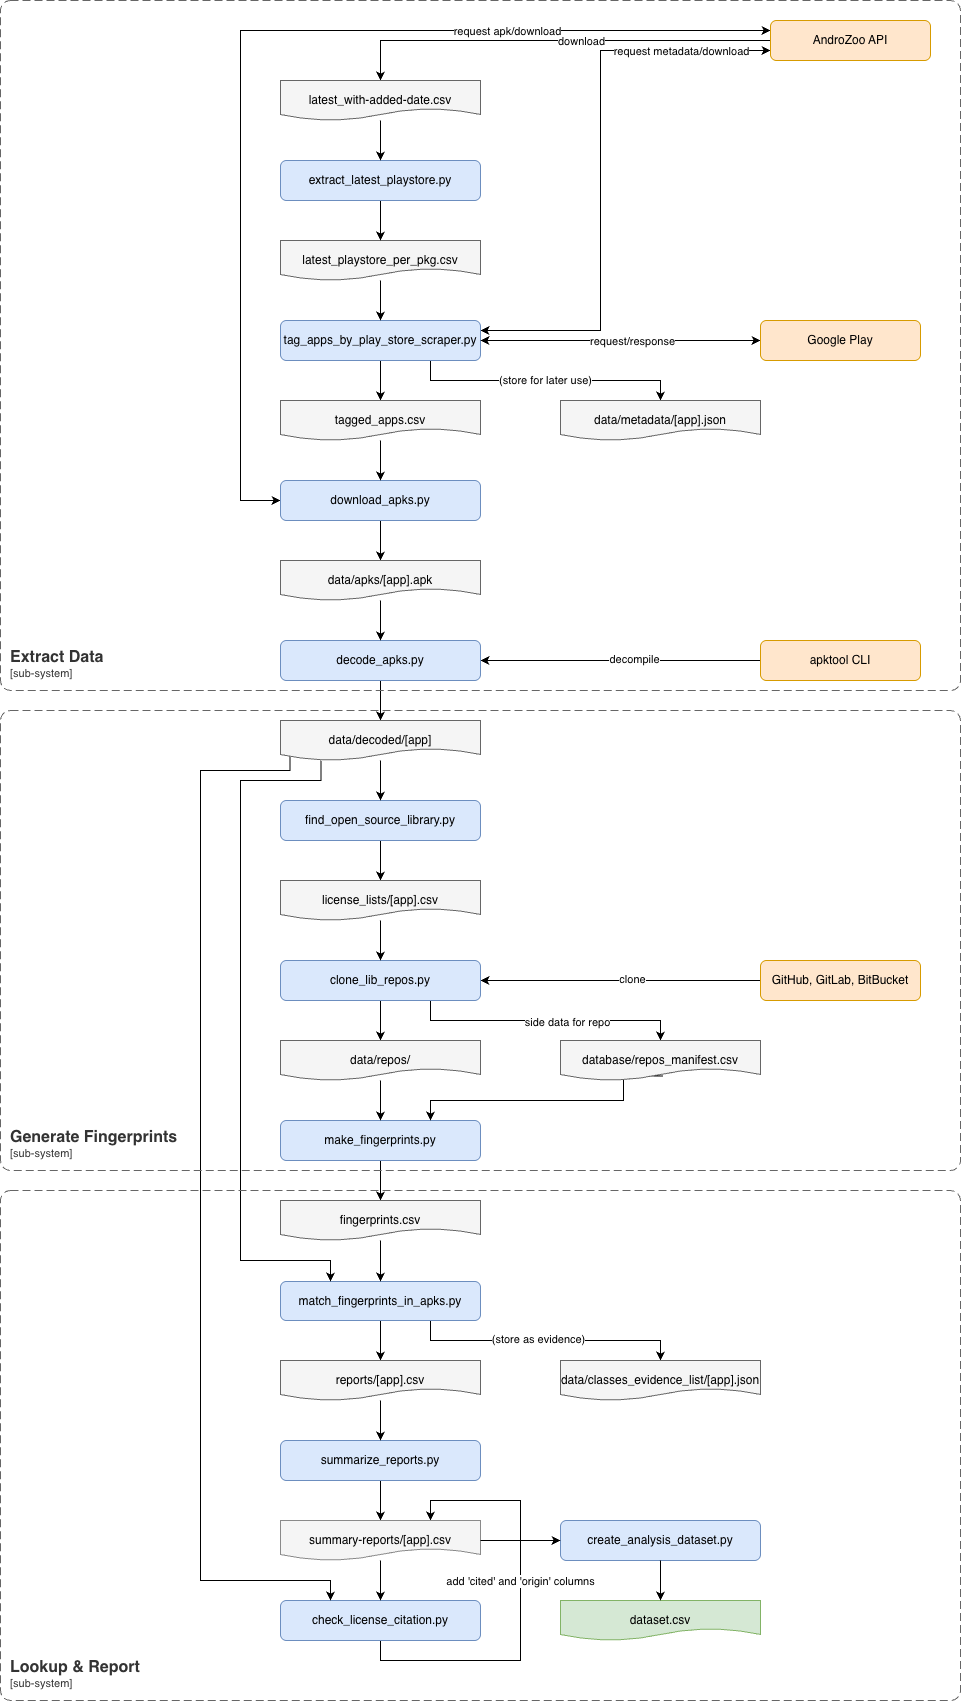
\includegraphics[width=\textwidth,height=0.78\textheight,keepaspectratio]{image/Analysis System_ Open Source Library in APKs.drawio.png}
    \caption{Overview of the data acquisition and analysis pipeline}
    \label{fig:pipeline}
\end{figure}

\section{Input Data Sources}
The primary source of APK files is the AndroZoo dataset, which provides large‑scale collections of Android applications together with metadata such as SHA256 hash, package name, and market origin. The dataset enables reproducible selection of applications and supports automated download through an API. 

In the first step, the large metadata CSV is filtered to keep only the most recent version of each application and to restrict the sample to apps available on Google Play. This filtering reduces the dataset size while preserving representative applications. Category information is then collected using a crawler to obtain official Google Play categories. The final dataset used in the pipeline contains only applications belonging to selected categories such as finance, healthcare, navigation, and communication, which are relevant for dependency and security analysis. 

\section{APK Acquisition and Decoding}
After the dataset is prepared, APK files are downloaded automatically using the AndroZoo API. Each APK is then decoded using the \texttt{apktool} utility, which converts the compiled application into a readable directory structure containing resources, manifest files, and smali code. Decoded applications are stored in a directory structure indexed by package name, which simplifies later lookup and cross‑matching. 

\section{License Extraction}
The next step searches the decoded project tree for license declarations. The workflow scans files for keywords such as \texttt{license} and extracts structured information including library name, repository URL, license type, and evidence path. The results are stored in per‑application CSV files. 

This step provides an initial list of candidate libraries, but license declarations alone are not sufficient because many applications use libraries without including explicit notices. Therefore, license extraction is only the first stage of library identification and must be combined with fingerprint‑based matching in later steps. 

\section{Repository Collection}
Libraries that contain repository URLs pointing to GitHub, GitLab, or Bitbucket are treated as public open‑source dependencies. Each unique repository is cloned locally to obtain the original source code of the library. This enables extraction of reliable identifiers from the library itself instead of relying only on declarations inside the APK. 

\section{Fingerprint Generation}
For each cloned repository, the pipeline scans the source tree for package declarations in Java and Kotlin files. Package names are extracted and stored as fingerprints that uniquely identify the library (Look at the logic in the Appendix Figure~\ref{fig:screenshot-make-fingerprints}). Additional support was later added for JavaScript libraries by detecting package declarations in distribution files, because some Android apps embed web components that are not visible through Java class matching (Look at the ratio of success for each fingerprint generation method based on final corpus analysis in the Appendix Figure~\ref{fig:fingerprint-type-ratio}).

All fingerprints are stored in a central CSV database containing the library name, repository URL, license information, and detected package prefixes. This database grows as more repositories are processed, increasing the probability of detecting libraries in later APK scans.

\subsection{Illustrative Example of Open-Source Library Detection}

To see how the generated fingerprints are used in practice, we can look at Glide as a simple example: a Java image-loading and bitmap-decoding library whose package namespace includes \texttt{com.bumptech.glide}.
Figure~\ref{fig:library-evidence-sample} shows one example from the decoded APK \texttt{com.rangebank.grip} AKA \textit{Range Bank}. The class \texttt{BitmapDrawableDecoder} was detected through export and import evidence. The license was not found in this APK, but the repository path for Glide was identified in another decoded APK at \texttt{data/decoded/hu.webvalto.bkkfutar/assets/licenses.json}.

\begin{figure}[htbp]
    \centering
    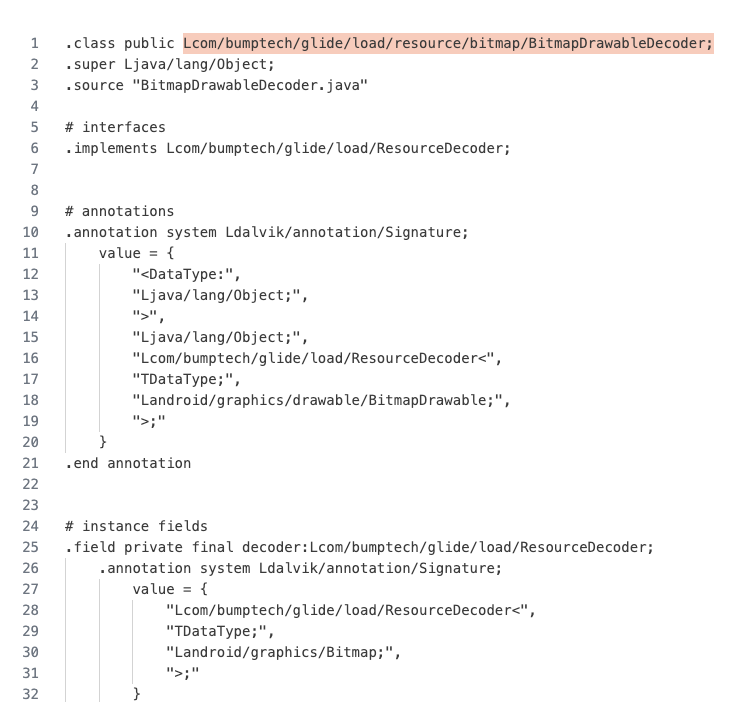
\includegraphics[width=0.48\textwidth,keepaspectratio]{image/Screenshot-library-export-evidence.png}\hfill
    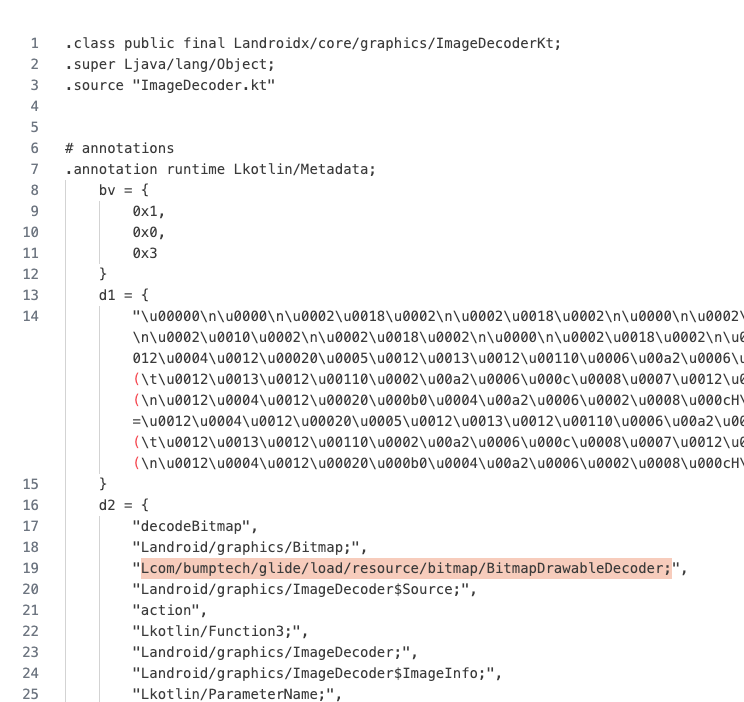
\includegraphics[width=0.48\textwidth,keepaspectratio]{image/Screenshot-library-import-evidence.png}
    \caption[Sample evidence of Glide library usage in a decoded APK]{Sample evidence of Glide library usage in a decoded APK}
    \label{fig:library-evidence-sample}
    {\footnotesize\textit{Note.} Left: export evidence at \texttt{data/decoded/com.rangebank.grip/smali_classes7/com/bumptech/glide/load/resource/bitmap/ BitmapDrawableDecoder.smali}. Right: import evidence at \texttt{data/decoded/com.rangebank.grip/smali/androidx/core/ graphics/ImageDecoderKt.smali}.}
\end{figure}


\section{Library Matching in APK Files}
The fingerprint-matching step is based on the principle that library imports and class definitions visible in the decoded codebase must originate from a defined package namespace (Figure~\ref{fig:library-evidence-sample}). Therefore, when the pipeline finds an import or class reference that matches the fingerprint of a known library, this is interpreted as evidence that the library is used in the APK.

After the fingerprint database is built, the pipeline scans decoded APK files for these import and class-definition references in smali code. The extracted paths are compared against stored package fingerprints using prefix matching. This step acts as the main detection gate: once library usage is identified, the later analysis checks whether the corresponding license was declared in the APK or whether the library was detected only through code evidence.

The matching step enables detection of both declared and undeclared libraries and was optimized using indexed lookup to reduce runtime when processing larger datasets.

\section{Aggregation and Reporting}
The final step aggregates all detected information into a unified report. For each application, the pipeline records detected libraries, license declarations, repository references, and matching evidence. The aggregated report also checks whether license notices appear close to the corresponding package usage or are stored in external assets, which helps evaluate compliance practices.

The reporting step also supports iterative improvement of the pipeline. When missing libraries are discovered, the repository list and fingerprint database can be extended and the matching step repeated without repeating the earlier stages. The final deliverable of this process is \texttt{dataset.csv}, where each row reports one APK-library relationship together with citation status and supporting evidence for the detected library.

\section{Computational Efficiency Techniques}
Several optimizations were introduced to make the pipeline practical for larger APK corpora. The most important improvement was to avoid repeatedly scanning every decoded file during lookup. Instead, for each decoded APK, the pipeline creates a compact evidence index containing only lines relevant to library imports, exports, and comments. Each indexed entry stores the file path, the original line of code, and the extracted import or class-reference evidence. This structure reduces the search space while preserving the information needed to prove library usage.

Fingerprint matching was also optimized by sorting class and package identifiers and using \textit{binary search} where possible. This made comparisons between decoded APK evidence and known library fingerprints more efficient than repeated linear scans. The same principle was applied in the final license-checking stage, where the pipeline must compare thousands of license records against a very large decoded corpus.

The performance gain was substantial. In the final corpus, 6,536 license records had to be checked against approximately 20 million decoded files. Initial tests showed that a direct lookup over this data could take more than 20 hours on a normal PC. After creating the evidence index and using optimized lookup techniques, the same process completed in approximately 156 minutes for the 700-APK corpus. These improvements made repeated experimentation and pipeline refinement feasible within the available hardware limits.

\chapter{Data Analysis}

\section{Generated Dataset}
The final dataset produced by the pipeline represents aggregated evidence of open‑source library usage across the analyzed APK corpus. Each row in the dataset corresponds to a detected library within a specific application, together with supporting evidence extracted from both license declarations and fingerprint matching.

The dataset contains the following key attributes:
\begin{itemize}
\item \textbf{pkg\_name}: identifier of the Android application
\item \textbf{repo\_host, repo\_path, repo\_url}: information about the source repository of the detected library
\item \textbf{library\_name}: human‑readable name of the library
\item \textbf{library\_key}: normalized identifier for grouping libraries
\item \textbf{cited}: binary indicator showing whether the library was declared via license (1) or only detected through fingerprints (0)
\item \textbf{origin}: method of detection (license, fingerprint, or both)
\item \textbf{smali\_prefix}: package prefix used for matching
\item \textbf{fingerprint\_types}: type of fingerprint used (e.g., Java, Kotlin)
\item \textbf{classes\_matched}: number of matched classes in the APK
\item \textbf{sample\_class, sample\_class\_file}: evidence of detection within the decoded APK
\end{itemize}

\subsection{Corpus Scaling Strategy}
To evaluate the robustness and scalability of the pipeline, the dataset was constructed incrementally using increasing corpus sizes. The number of analyzed APKs was expanded stepwise as follows:

\begin{center}
[10, 20, 30, 40, 60, 80, 100, 150, 200, 300, 500, 700]
\end{center}

This approach allows observation of how key metrics evolve as more applications are included, and whether the results stabilize at larger scales.

\subsection{Evaluated Metrics}
The following key performance indicators (KPIs) were extracted from the dataset at each corpus size:

\begin{itemize}
\item Number of detected libraries per APK
\item Ratio of declared vs. undeclared libraries
\item Number of unique libraries discovered
\item Growth rate of newly discovered libraries
\item Ratio of detection methods, comparing fingerprint-based evidence with license-based evidence
\item Average number of matches per library (classes\_matched)
\end{itemize}

\subsection{Observed Trends}
The scaling analysis reveals several important patterns:

\begin{itemize}
\item The number of detected library occurrences per APK increases slowly across corpus sizes, although the available data does not show the exact point at which this metric fully stabilizes (Figure~\ref{fig:library-occurrence-rows-per-apk}).
\item The number of unique libraries continues to grow with dataset size, but with diminishing returns, indicating that the most common libraries are discovered early (Figure~\ref{fig:unique-libraries-growth}) (Total numbers available in appendix Figure~\ref{fig:total-libraries-occurrences}.)
\item A significant portion of libraries are detected through fingerprint matching, suggesting that license declarations alone are incomplete in many applications (Figure~\ref{fig:fingerprints-vs-license-exposure}).
\item The ratio between declared and undeclared libraries becomes relatively stable from the 300-APK corpus onward, indicating consistent behavior across larger samples (Figure~\ref{fig:declared-vs-undeclared}).
\item Larger corpora improve the coverage of the fingerprint database and can increase detection accuracy, but the current 700-APK cap does not allow a precise conclusion about the final stabilization point.
\end{itemize}

The following figures illustrate the trends observed during scaling the corpus.

\begin{figure}[htbp]
    \centering
    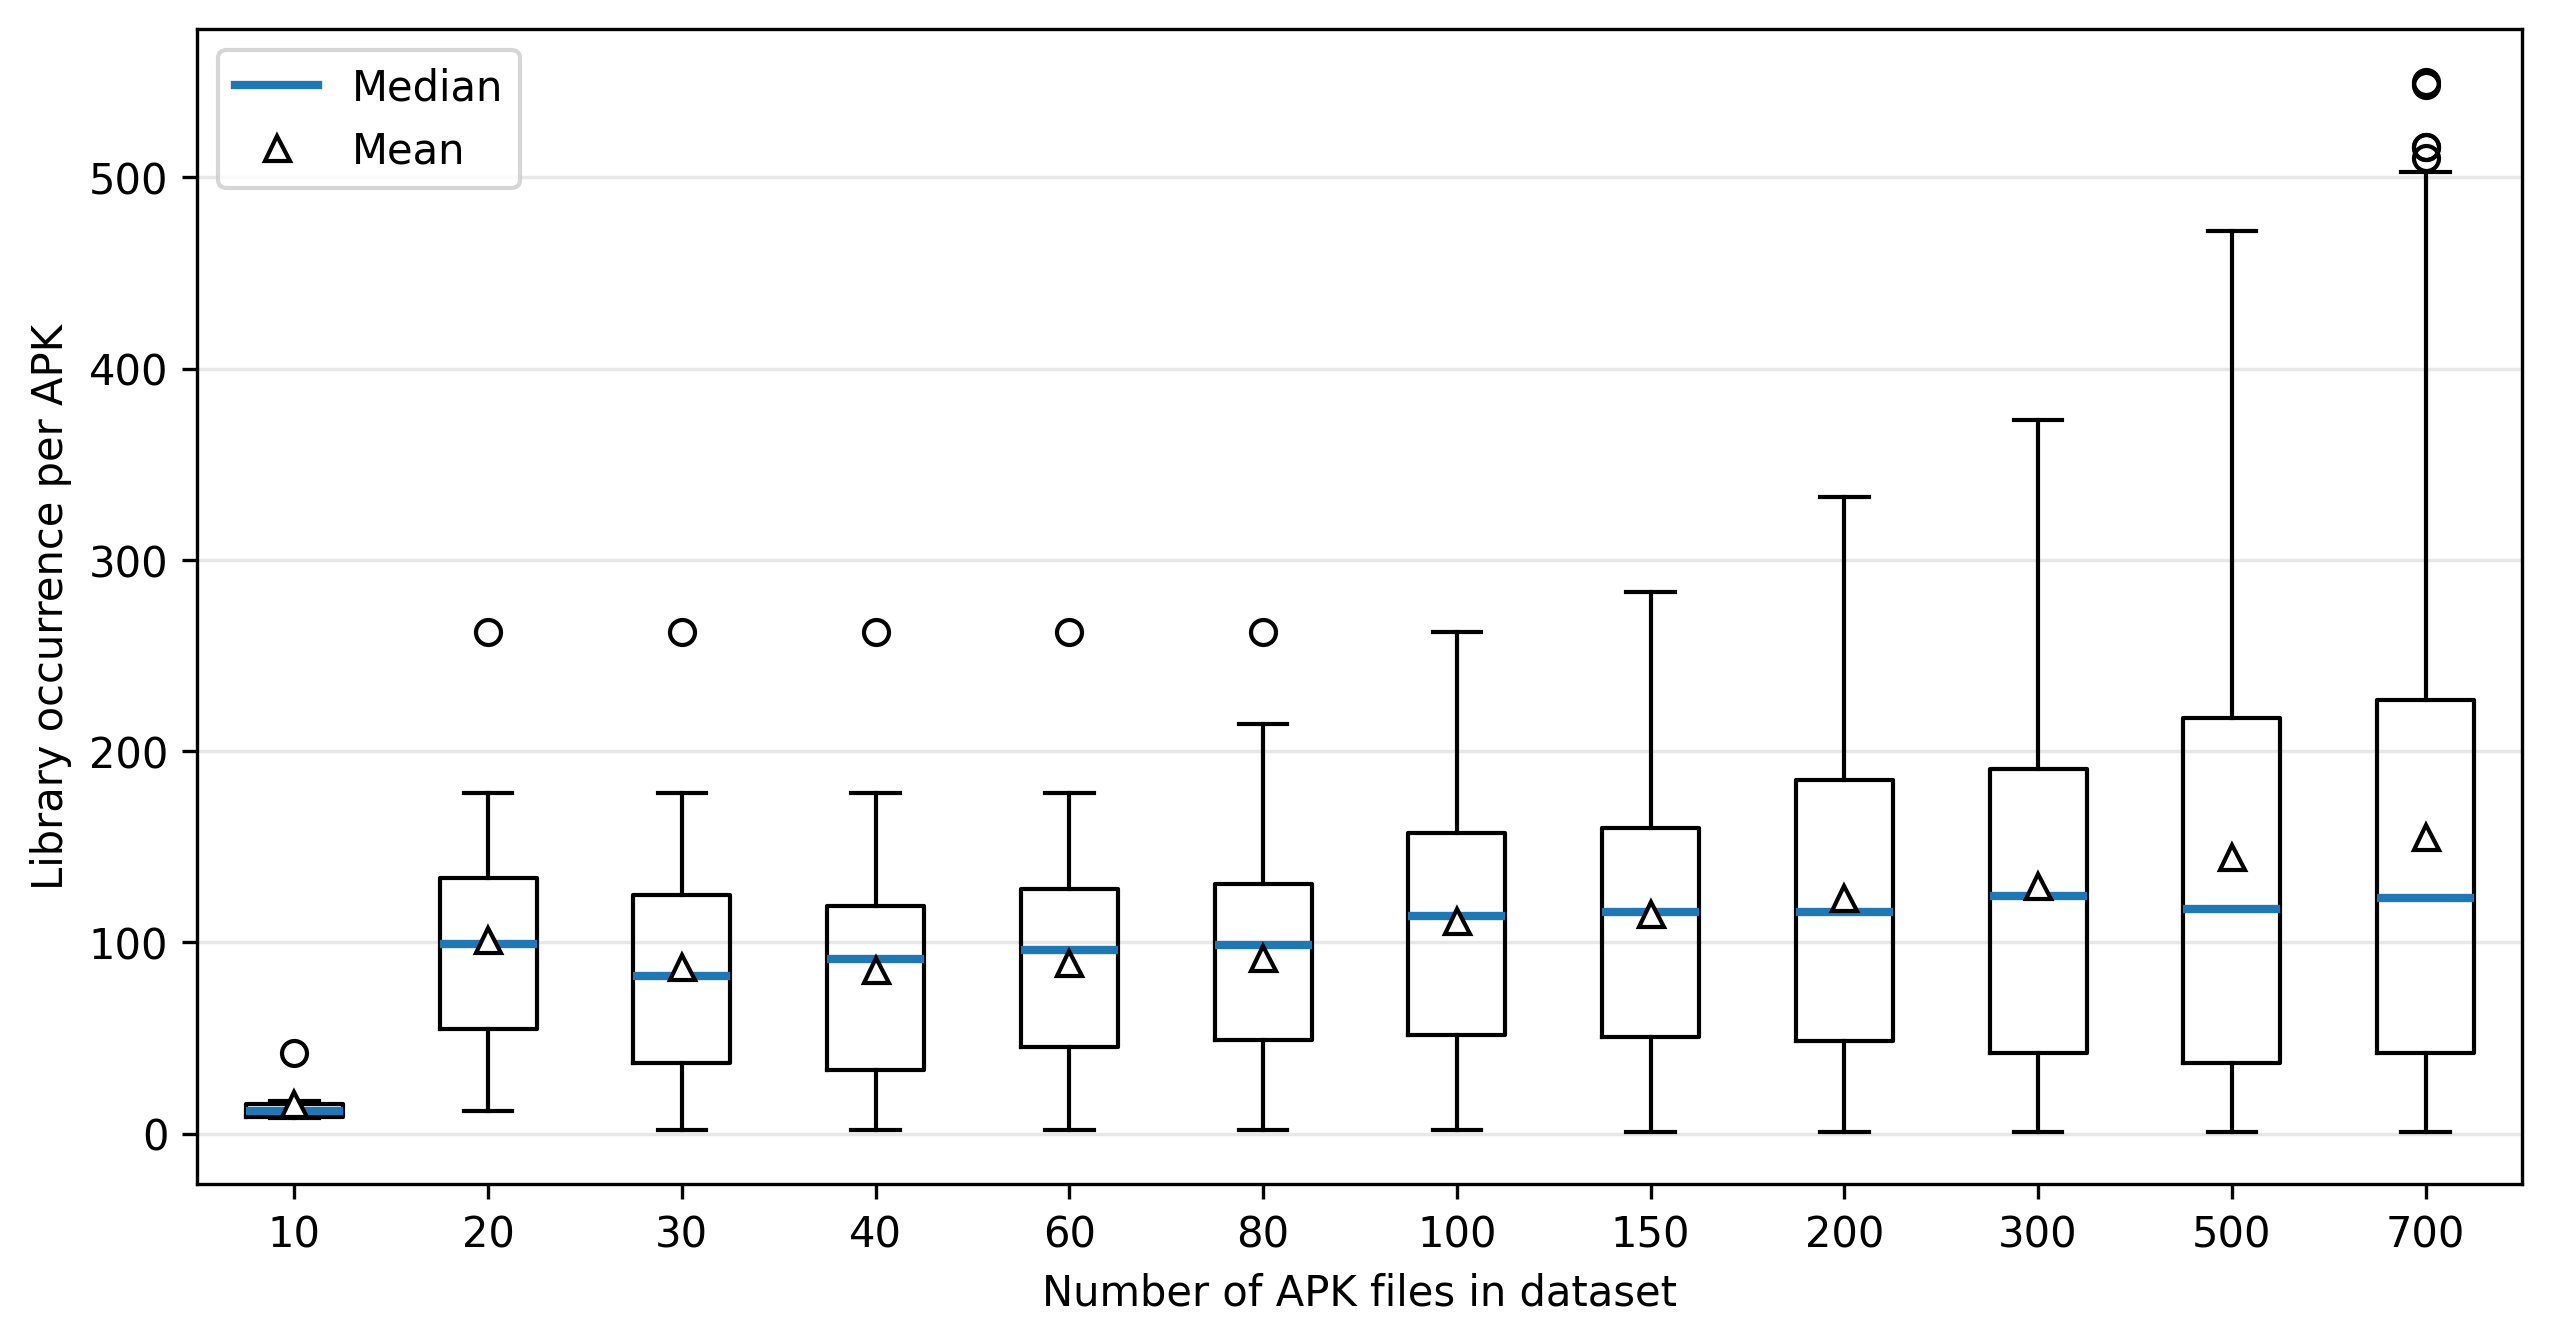
\includegraphics[width=\textwidth,keepaspectratio]{image/library_occurrence_rows_per_apk_distribution_boxplot.png}
    \caption{Distribution of library occurrence rows per APK}
    \label{fig:library-occurrence-rows-per-apk}
    \end{figure}
    
\begin{figure}[htbp]
    \centering
    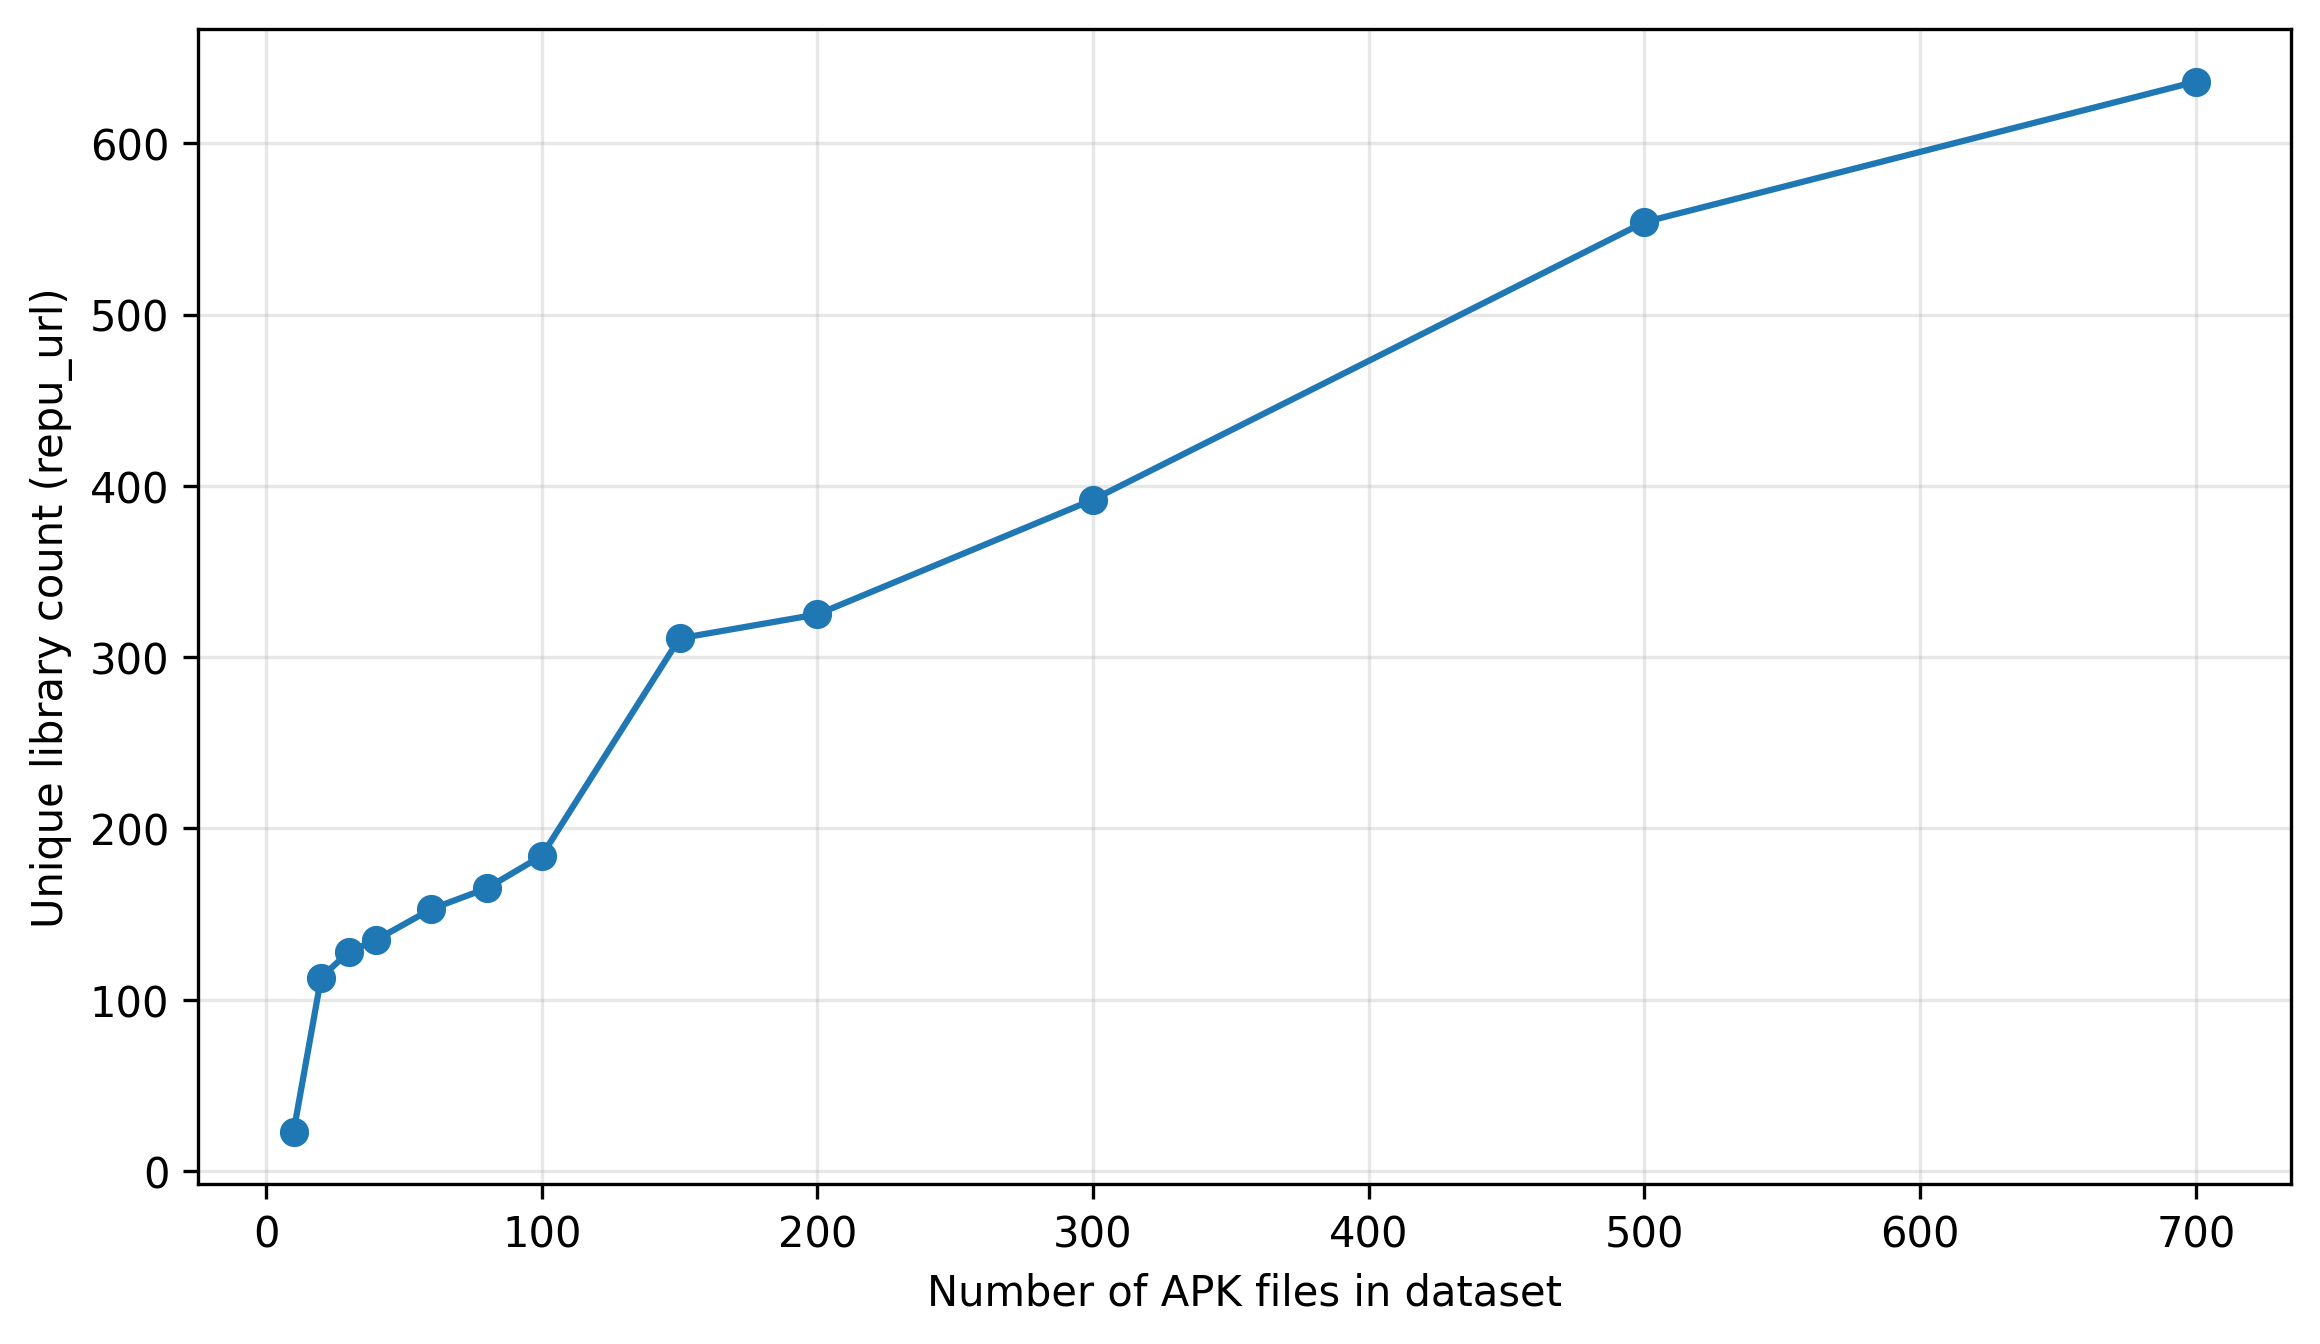
\includegraphics[width=\textwidth,keepaspectratio]{image/unique_open_source_libraries_by_apk_collection_size.png}
    \caption{Growth of unique libraries discovered as corpus size increases}
    \label{fig:unique-libraries-growth}
    \end{figure}

\begin{figure}[htbp]
    \centering
    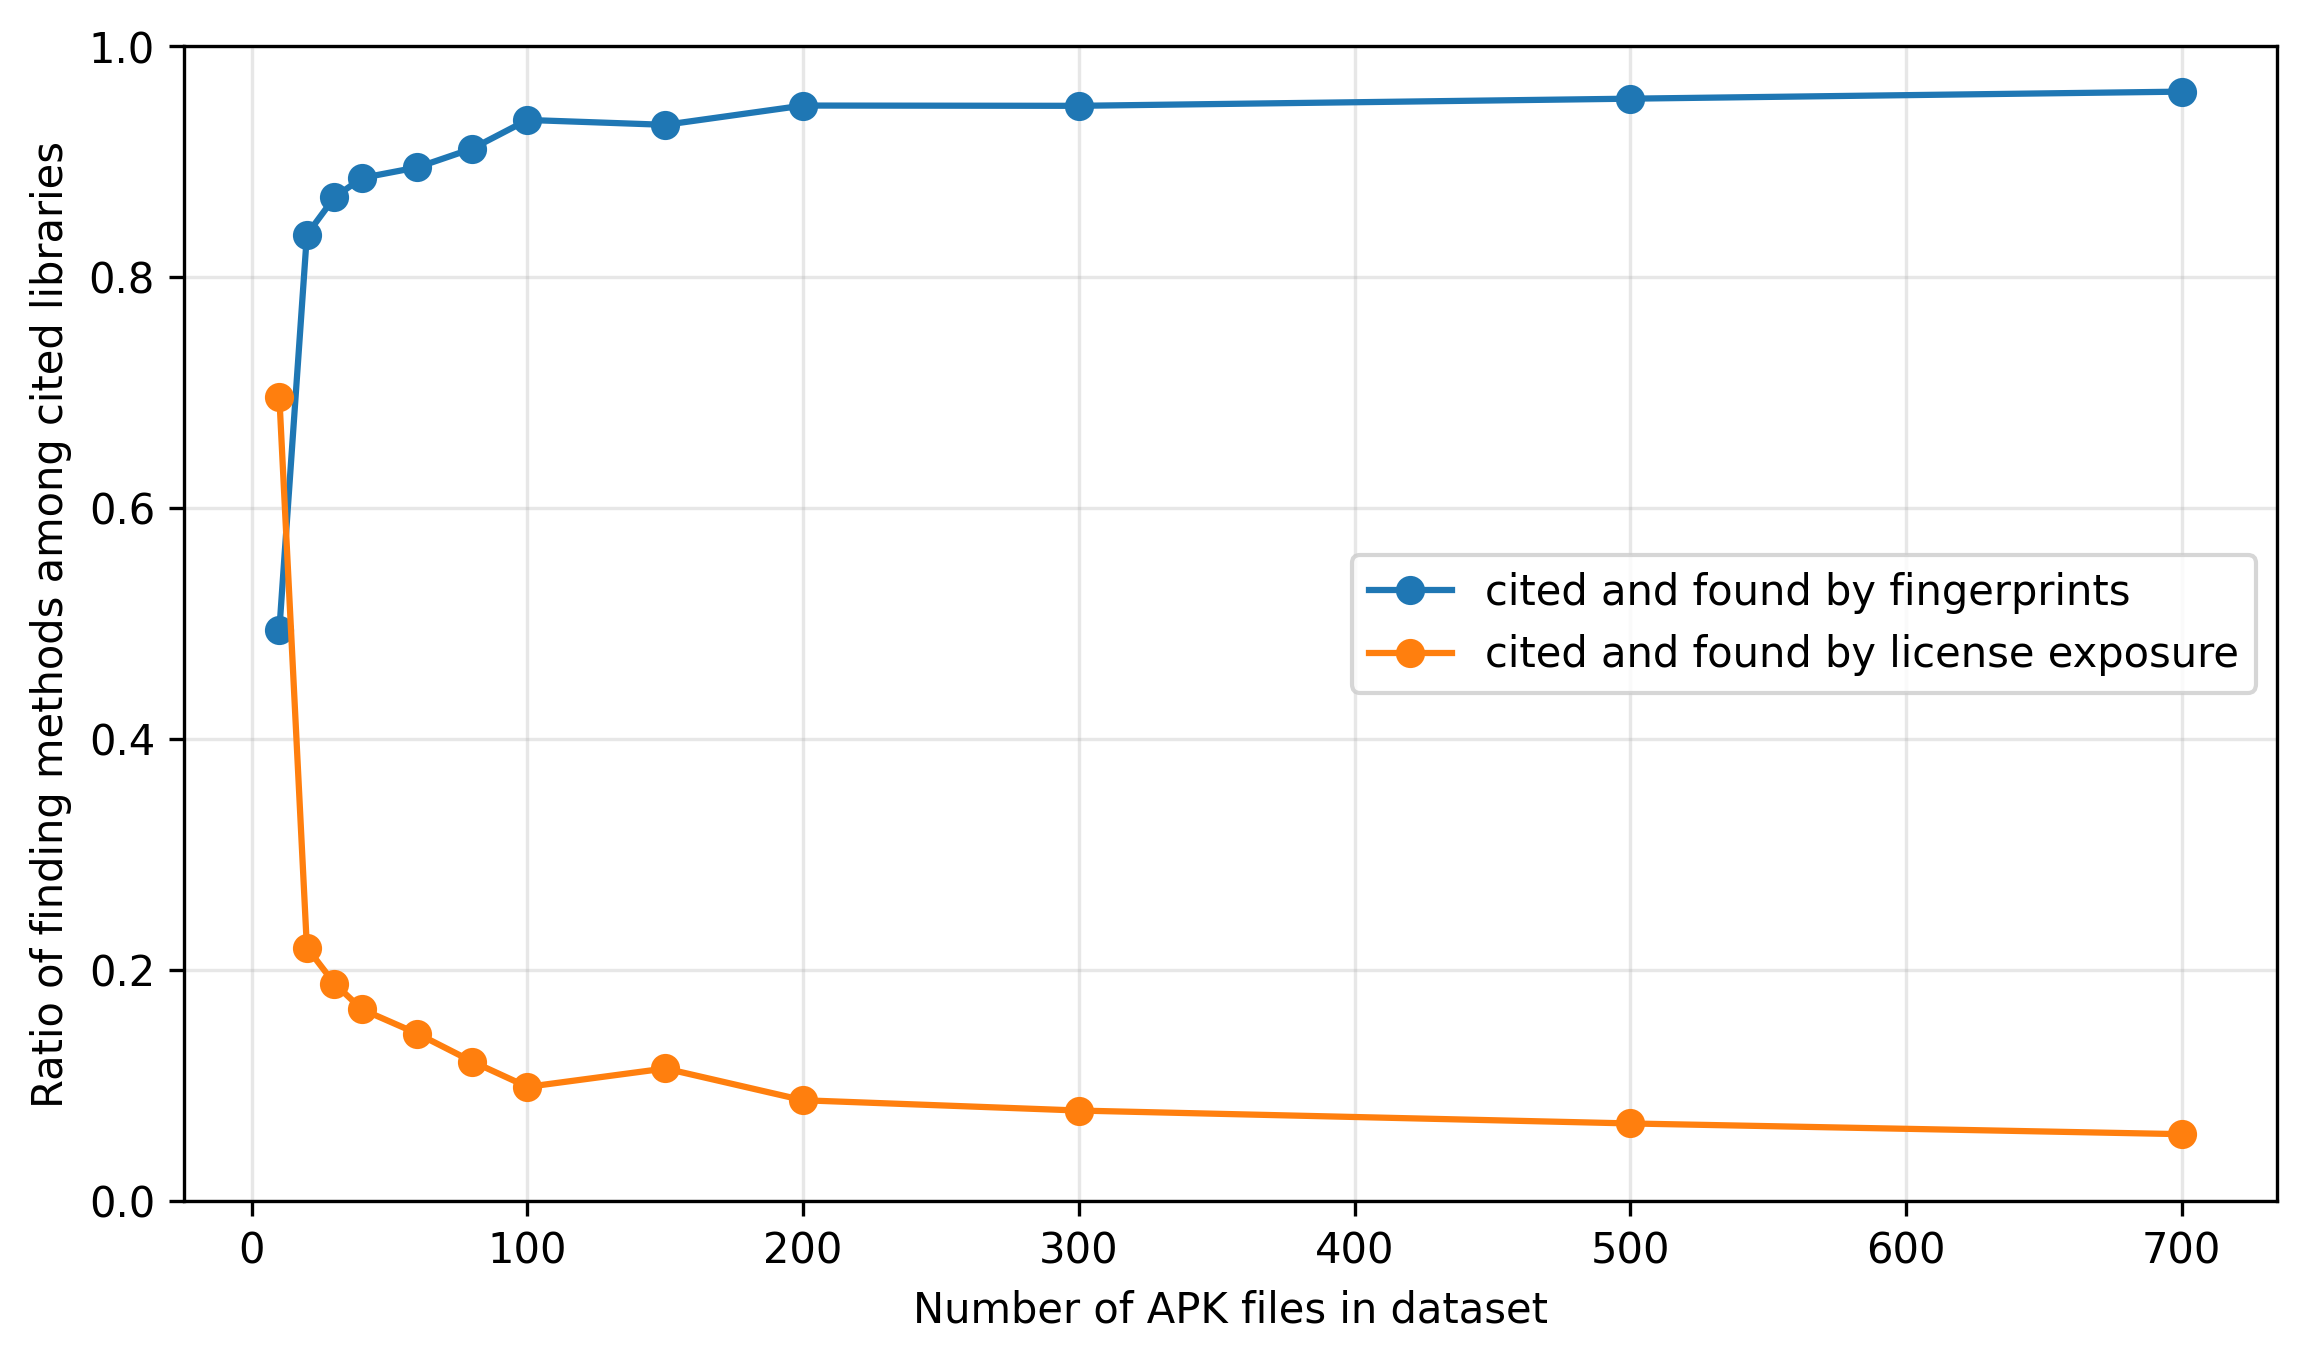
\includegraphics[width=\textwidth,keepaspectratio]{image/origin_coverage_among_cited_rows_by_apk_collection_size.png}
    \caption{Share of cited library records also confirmed by fingerprint evidence across corpus sizes}
    \label{fig:fingerprints-vs-license-exposure}
    \end{figure}

Figure~\ref{fig:fingerprints-vs-license-exposure} shows that from the 100-APK corpus onward, more than 90\% of cited libraries are also detected through fingerprint matching. This supports the pipeline assumption that a license declaration and repository URL found in one APK can be used to build fingerprints from the original source repository and detect the same open-source library in other APKs.


\begin{figure}[htbp]
\centering
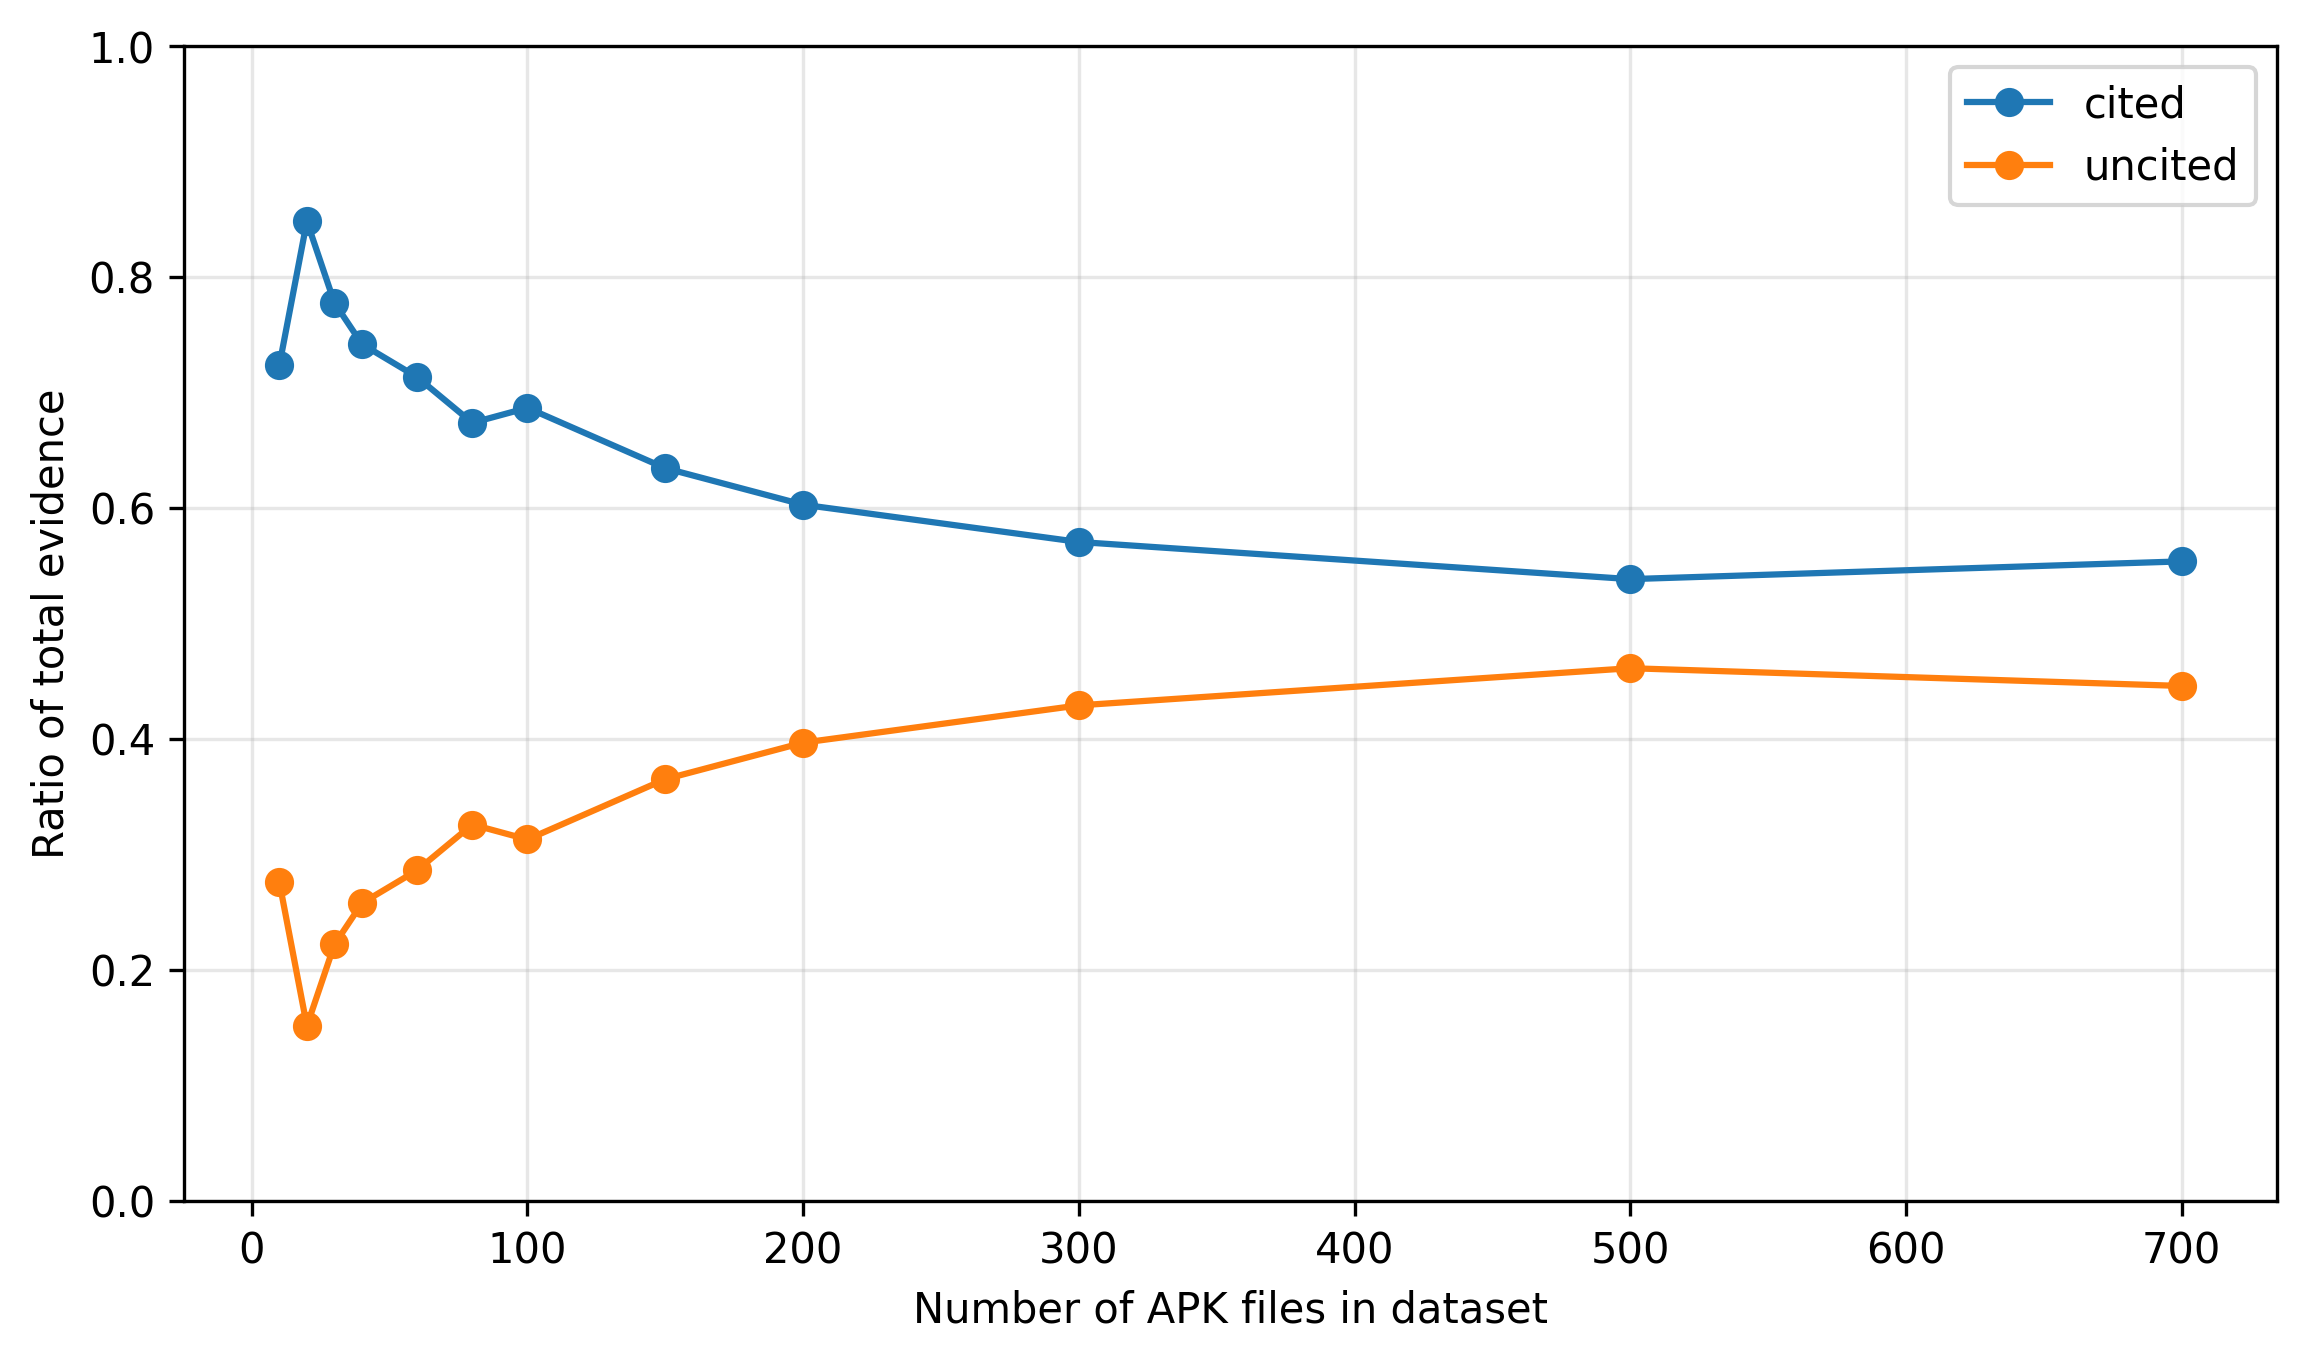
\includegraphics[width=\textwidth,keepaspectratio]{image/cited_ratio_by_apk_collection_size.png}
\caption{Ratio of declared vs. undeclared libraries across corpus sizes}
\label{fig:declared-vs-undeclared}
\end{figure}



\subsection{Final Dataset Selection}
Based on the scaling analysis we saw above, and considering the hardware resource limitation, the final corpus contains 699 APKs after one APK was excluded because its lookup process exceeded the time limit (Table~\ref{tab:apk-category-counts}). As we can also see from the category counts, the sample was not balanced by category. The pipeline selected applications from the target research categories according to availability in the AndroZoo input list and download execution, without imposing a preferred category distribution.

\begin{table}[htbp]
\centering
\caption{APK count by Google Play category in the final corpus}
\label{tab:apk-category-counts}
\begin{tabular}{lr}
\hline
\textbf{Category} & \textbf{APK count} \\
\hline
FINANCE & 289 \\
HEALTH\_AND\_FITNESS & 206 \\
COMMUNICATION & 83 \\
MAPS\_AND\_NAVIGATION & 65 \\
MEDICAL & 56 \\
\hline
\textbf{Total} & \textbf{699} \\
\hline
\end{tabular}
\end{table}

\section{GitHub-Based Repository Health Score}

After analyzing APK-level metrics, the we to repository-level evaluation using GitHub data. Prior studies show that open-source project health cannot be evaluated from a single raw repository attribute. \parencite{diruscioOSSMETERSoftwareMeasurement2015} present OSSMETER as a platform for automatically analysing OSS projects across multiple information sources, including source-code repositories, communication channels, and issue trackers. Their work is relevant because it frames OSS assessment as a multi-source measurement problem covering quality, maturity, development activity, and user support rather than only repository popularity.

A more direct health-score approach is proposed by \parencite{jiangMetricsEvaluateHealth2019}, who use GitHub data and factor analysis to evaluate OSS project health. Their model transforms basic repository indexes into six synthetic health-related metrics: community activity, project popularity, development activity, completeness, responsiveness, and persistence. This is important for the present thesis because it shows that repository health can be represented through combined indicators derived from project activity and community behavior.

Building on this line of work, \parencite{wangMethodEvaluateHealth2022} provide the most suitable model for this thesis because they define an explicit OSS project health score, organize the indicators into the pressure--state--response model, and report final weights for the selected factors. Therefore, this thesis adopts the Wang and Wu health-score method as the repository-level metric used for the detected GitHub libraries.

\subsection{Adopted Health-Score Model}

\textcite{wangMethodEvaluateHealth2022} propose a method for evaluating the health of open-source software projects based on the pressure--state--response (PSR) model. Their model divides repository health into three categories: pressure, state, and response. Across these categories, they define 12 factors (see Table~\ref{tab:wang2022-health-factors}). The full explanation of the Wang and Wu model, including its theoretical background and data-collection logic, will be provided in Appendix~\ref{app:wang2022-health-model}.

Table~\ref{tab:wang2022-health-factors} summarizes the 12 factors adopted in this thesis. The impact column indicates whether a larger value improves the health score (+) or reduces it (-). The weights are the final combined weights reported by Wang and Wu after combining AHP and entropy weighting.

\begin{table}[htbp]
\centering
\caption{Repository health factors adopted from Wang and Wu's OSS health model}
\label{tab:wang2022-health-factors}
\begin{tabular}{llcr}
\hline
\textbf{Factor title} & \textbf{Category} & \textbf{Impact} & \textbf{Weight} \\
\hline
Number of watches & Pressure & + & 0.0901 \\
Number of forks & Pressure & + & 0.1519 \\
Number of languages & Pressure & - & 0.2291 \\
Number of bugs & Pressure & - & 0.5285 \\
Number of contributors & State & + & 0.3147 \\
Number of commits & State & + & 0.1304 \\
Number of comments & State & + & 0.0676 \\
Number of issues & State & + & 0.4871 \\
Number of pull requests & Response & + & 0.0559 \\
Pull requests merged & Response & + & 0.3525 \\
Issue close/open ratio & Response & + & 0.4261 \\
Issue close time & Response & - & 0.1650 \\
\hline
\end{tabular}
\end{table}

\subsection{Application to Repositories Detected in the APK Corpus}

I adopted Wang and Wu method for the GitHub repositories identified through the APK-library detection pipeline. Starting from the repository URLs extracted from the final APK dataset, the pipeline collects repository-level information using the GitHub API and, where necessary, local cloned repositories. The APK corpus contains 274 unique GitHub repository URLs. The health-score data collection successfully gathered the required indicators for 220 repositories, while 54 repositories were excluded or marked incomplete because of missing data, unavailable repositories, API errors, or incompatible repository structure (reflected as nan in Figure~\ref{fig:github-wang2022-health-level-distribution}).

For each repository, the 12 factors are normalized before the layer scores are calculated. This step is necessary because the factors use different scales. For example, forks, commits, and comments are count variables, while issue close time is measured in days. Following Wang and Wu, positive factors are normalized as:

\begin{equation}
 a'_i = \frac{a_i - \min(a)}{\max(a) - \min(a)}
\end{equation}

Negative factors are normalized in the opposite direction:

\begin{equation}
 a'_i = \frac{\max(a) - a_i}{\max(a) - \min(a)}
\end{equation}

This means that higher normalized values always represent better health. For example, the minimum number of forks in the repository dataset is 0 and the maximum is 78,914, in \textit{BoltsFramework/Bolts-Android} with 535 forks receives the normalized positive value:

\begin{equation}
 \frac{535 - 0}{78914 - 0} = 0.0068
\end{equation}

In contrast, issue close time is treated as a negative factor, and the minimum close time is 0.01 day while the maximum is 2621 days, in \textit{BoltsFramework/Bolts-Android} with an average close time of 55.24 days receives:

\begin{equation}
 \frac{2621 - 55.24}{2621 - 0.01} = 0.9789
\end{equation}

After normalization, the pressure, state, and response scores are calculated as weighted sums of their respective factors. The final repository health score is then calculated as the average of the three layer scores multiplied by 100:

\begin{equation}
 H = \left(\frac{H_P + H_S + H_R}{3}\right) \times 100
\end{equation}

\subsection{Repository Health-Score Results}

The resulting health score provides a single value for each repository, where a higher score indicates a healthier repository. Figure~\ref{fig:github-wang2022-top-healthiest} shows the top 10 healthiest repositories in the APK corpus.

\begin{figure}[htbp]
\centering
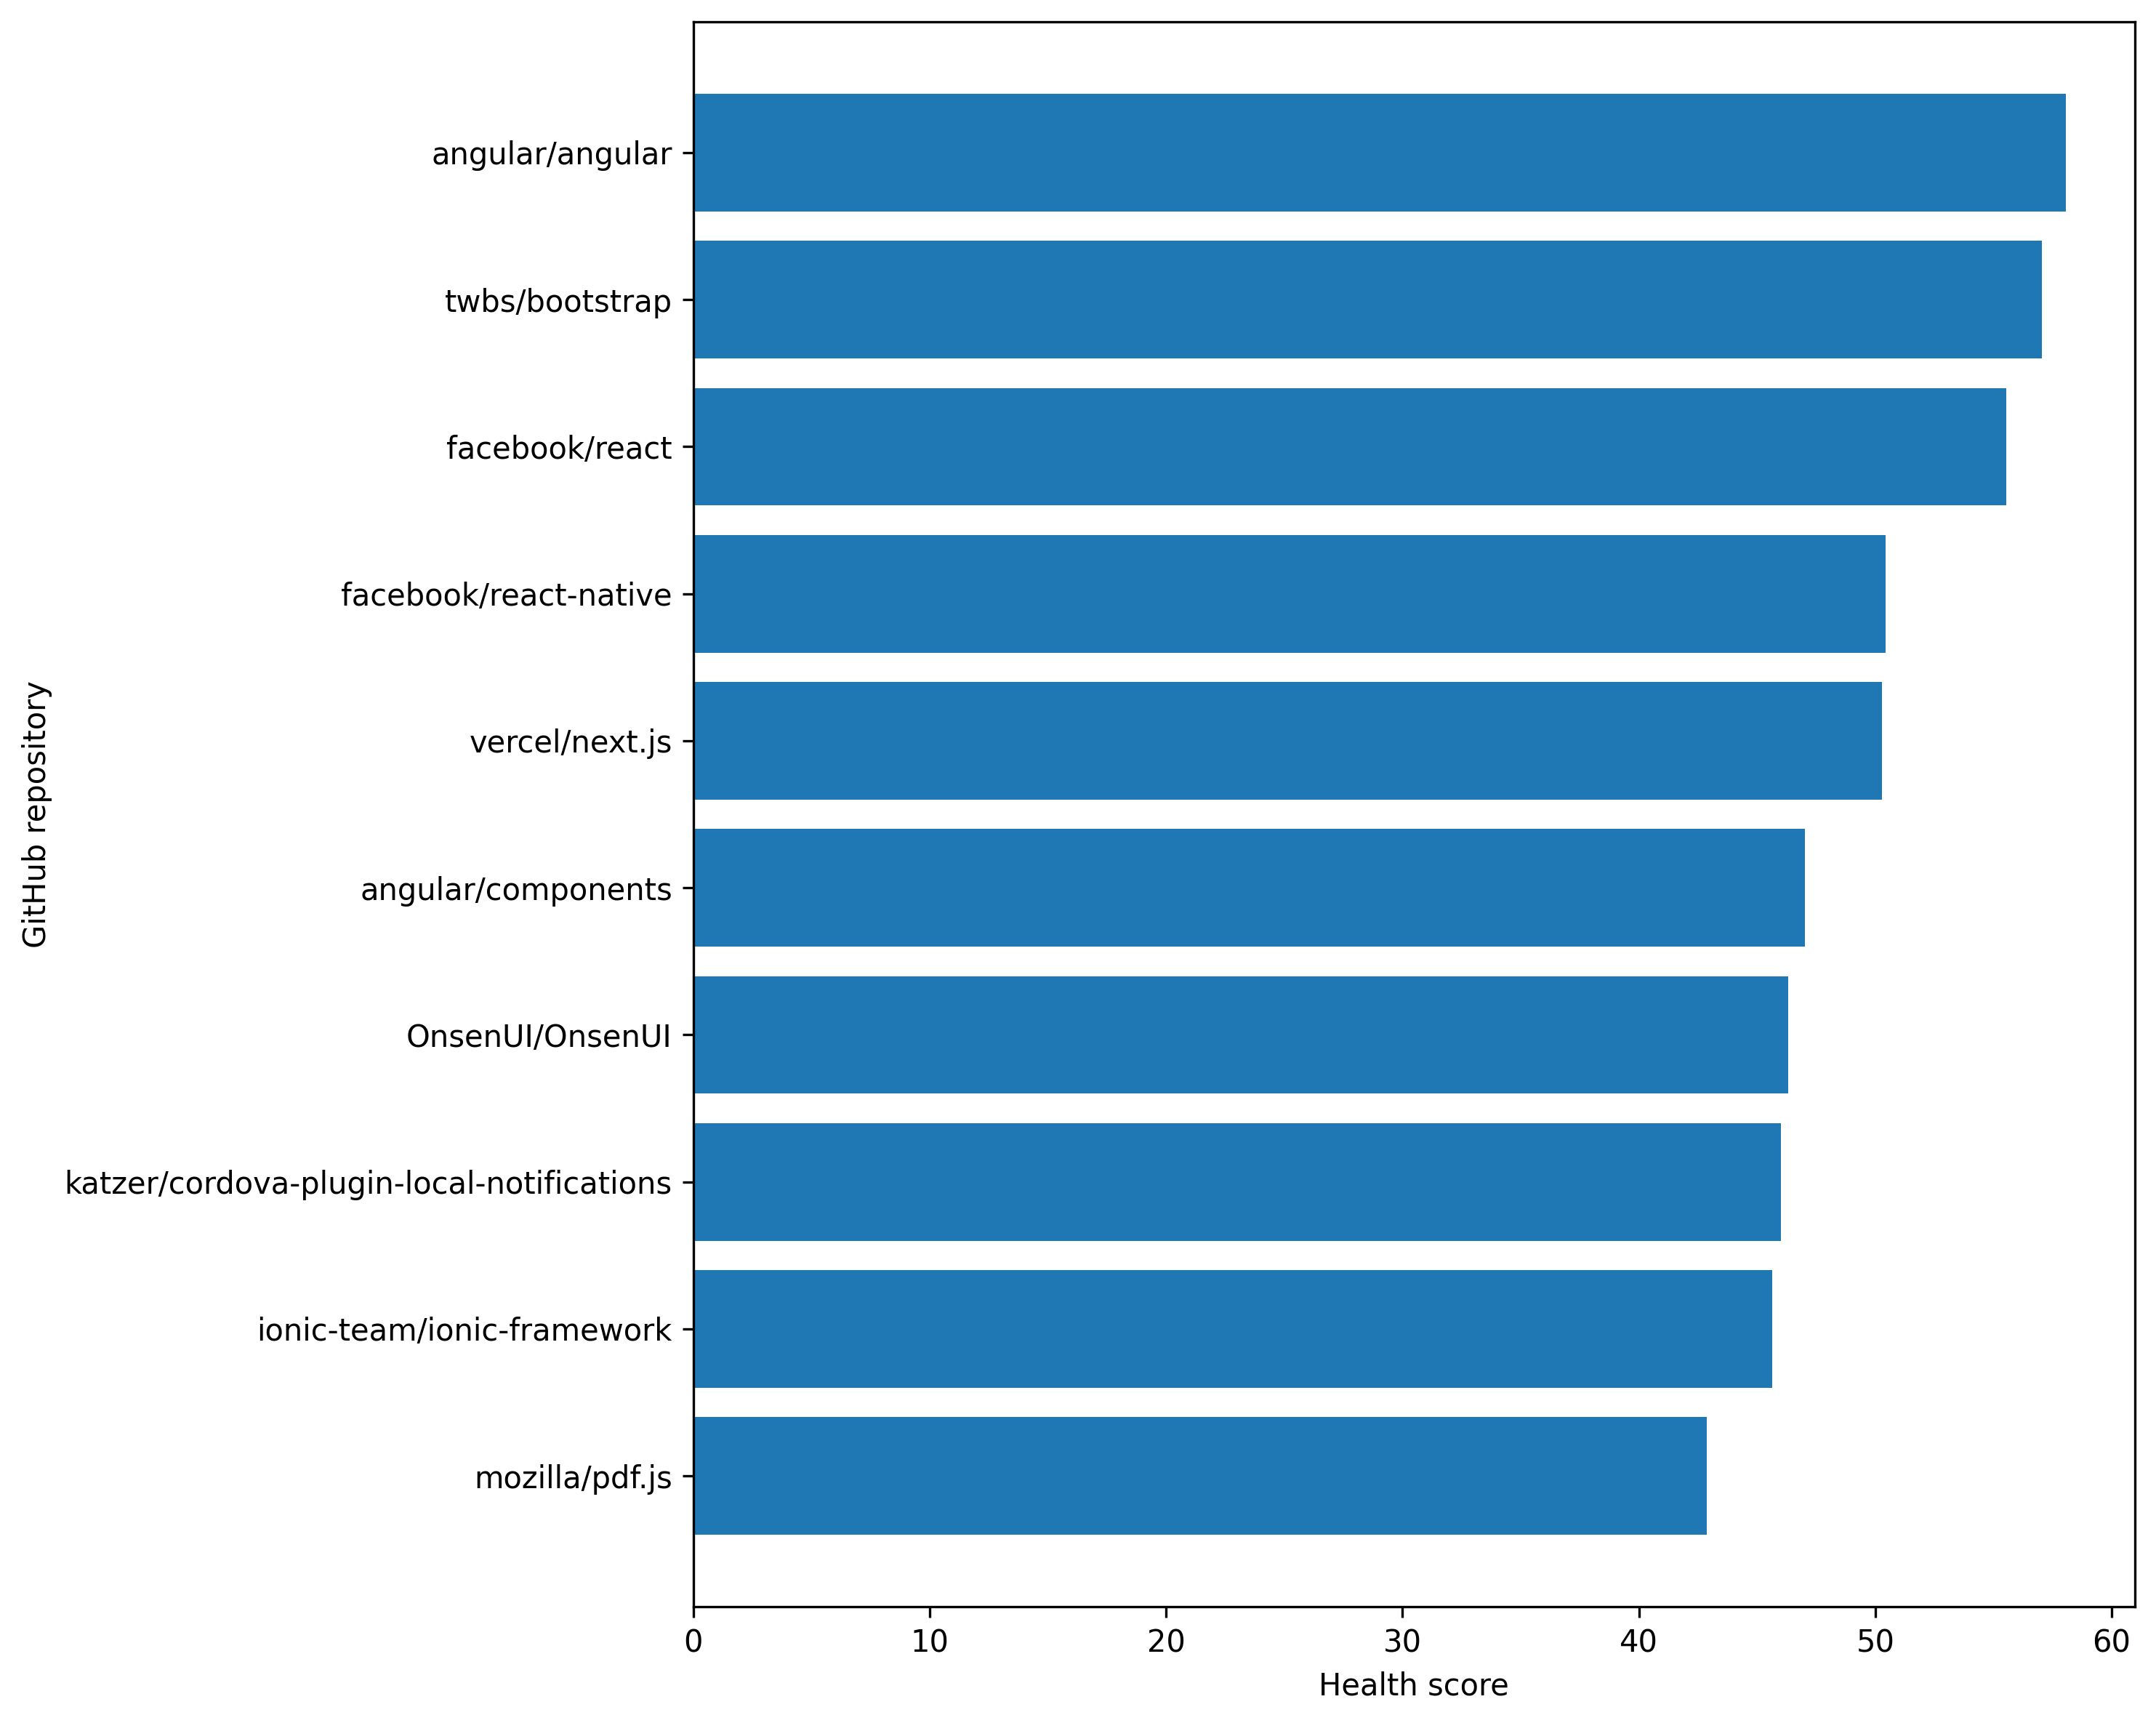
\includegraphics[width=0.75\textwidth,keepaspectratio]{image/top_repositories_by_health_score.png}
\caption{Top 10 repositories health score in the APK corpus}
\label{fig:github-wang2022-top-healthiest}
\end{figure}

Wang and Wu divide repository health scores into three levels: low health in the interval [0, 10), medium health in the interval [10, 30), and high health in the interval [30, 100]. This thesis adopts the same thresholds so that the resulting repository categories remain consistent with the source model. In the analyzed GitHub repository set, no repository falls into the low-health category, 16 repositories fall into the medium-health category, and 204 repositories fall into the high-health category. Figure~\ref{fig:github-wang2022-health-level-distribution} shows the distribution of repositories across these health levels in the APK corpus.

\begin{figure}[htbp]
\centering
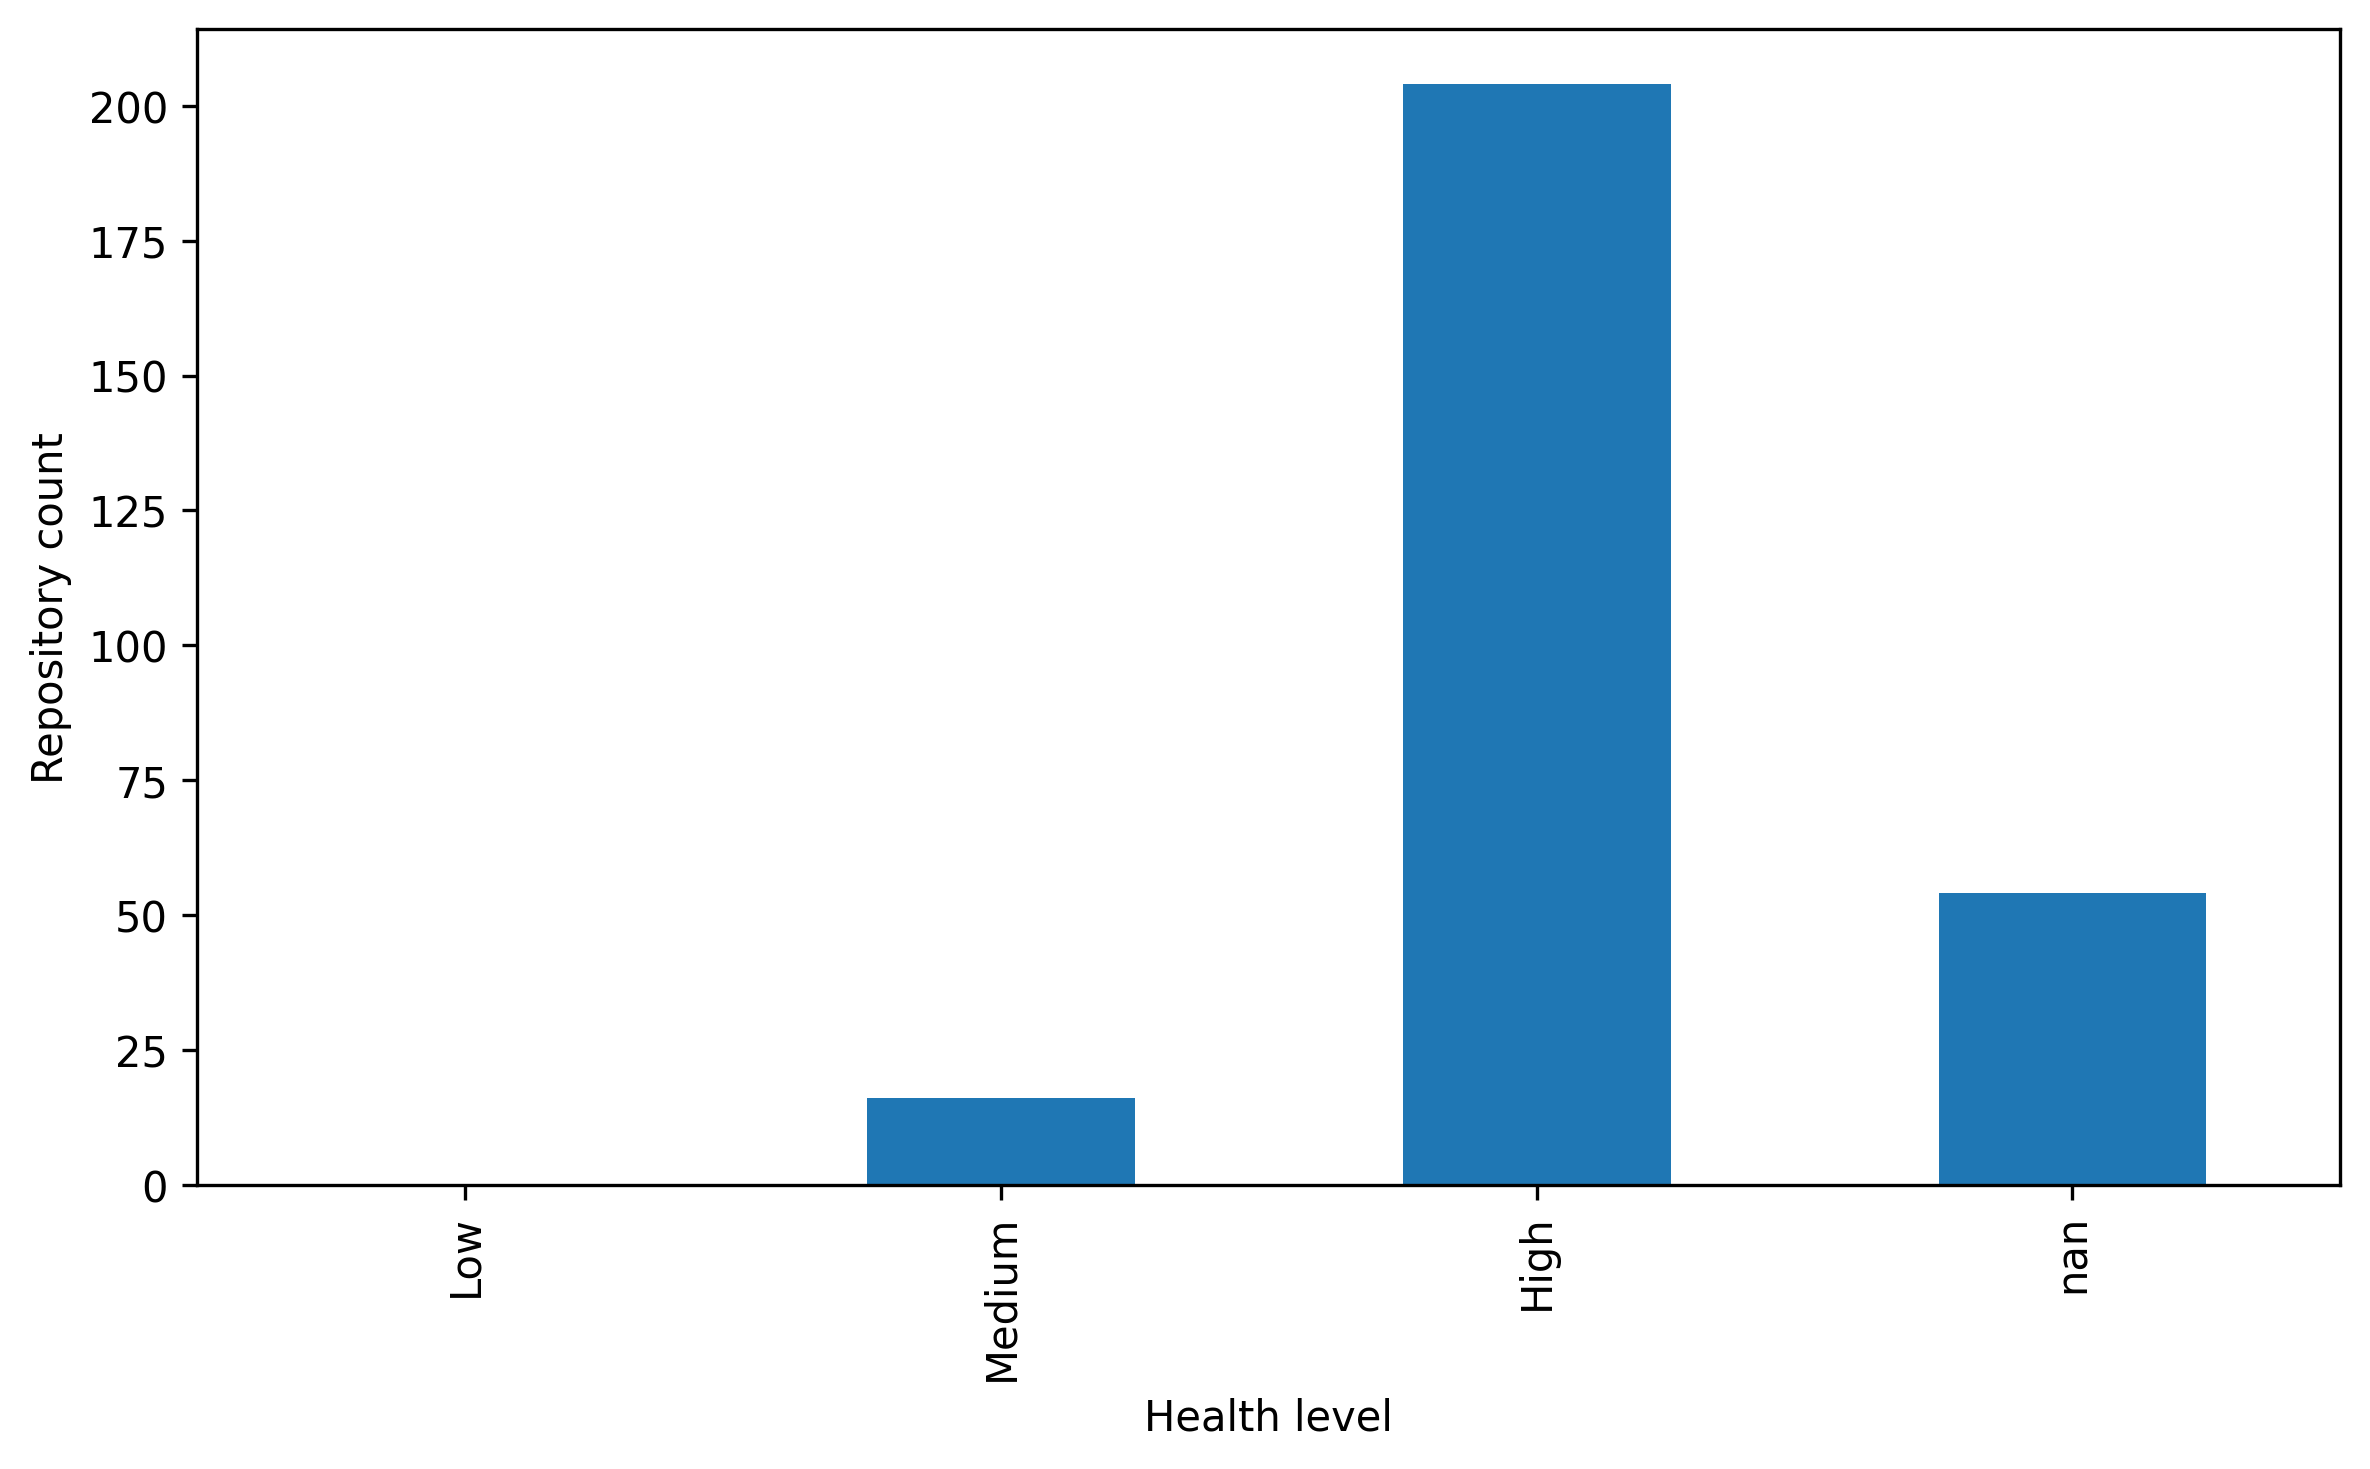
\includegraphics[width=0.7\textwidth,keepaspectratio]{image/repository_count_by_health_level.png}
\caption{Distribution of repositories across health levels in the APK corpus}
\label{fig:github-wang2022-health-level-distribution}
{\footnotesize\textit{Note.} The \texttt{nan} category represents repositories that were excluded or marked incomplete because of missing data, unavailable repositories, GitHub API errors, or incompatible repository structure.}
\end{figure}

The repository-level health data will later be joined back to the APK-library evidence dataset. This makes it possible for us to estimate which APKs depend on medium-health libraries and how intense those libraries appear in each APK. The APK-level interpretation of this joined dataset is discussed later in Subsection~\ref{sec:medium-health-level-open-source-library-usage-in-apks}.


\chapter{Validation}

\section{Validation Strategy}
At this point, the pipeline has identified open-source libraries used in each analyzed APK through license extraction and fingerprint matching. The main validation question is whether these detected libraries can be compared against an independent baseline. Initially, the planned validation approach was to inspect applications manually and compare the pipeline output with the list of open-source libraries disclosed inside the application itself. This would have provided a direct user-visible validation source if applications exposed their dependency declarations through an in-app license screen.

However, this first validation strategy was not successful as a general baseline. A sample of 27 commercial applications (Appendix Table~\ref{tab:list-apps-manual-validation}) was installed and explored manually in the Android Studio Emulator, including settings menus, about pages, help pages, and other sections where open-source notices are typically located. Almost none of the selected applications provided an accessible in-app list of open-source libraries. The only clear exception was \textit{BudapestGO}, where the in-app license screen matched the libraries detected by the pipeline (Appendix Table~\ref{tab:budapestgo-summary-report}). This result was useful as a qualitative example, but it was not sufficient for estimating accuracy, precision, recall, or false positives across the pipeline.

For this reason, a second validation approach was introduced using open-source Android applications from F-Droid. The motivation was to create a control set where the APK can be analyzed by the fingerprinting pipeline, while the corresponding public source-code repository can be inspected independently. In this setting, the source-code analysis is treated as an approximate ground truth because dependencies may be declared in Gradle files, version catalogs, third-party documentation, vendor directories, or repository references. The validation therefore compares two independent sources of evidence for the same applications: libraries detected from the compiled APK and libraries reconstructed from the public source code.

\section{Open-Source Control Set}
The validation control set consists of 100 F-Droid applications. These applications were selected from the F-Droid dataset under three conditions. First, the package name had to exist in the main APK input dataset (AndroZoo). Second, the application had to belong to one of the research categories used in the main corpus. Third, the F-Droid metadata had to contain a GitHub source-code URL. This ensured that each selected application had both an APK representation for pipeline analysis and a source-code repository for independent comparison.

The APK analysis pipeline was then executed separately for these 100 F-Droid applications. For this validation run, the fingerprint database was not limited to fingerprints generated from the F-Droid repositories alone. Instead, it combined the fingerprints already gathered from the main 699-APK corpus with the additional fingerprints generated from the 100 F-Droid APKs and their related source-code evidence. This design made the validation run closer to the real pipeline setting, because the APKs were analyzed against the accumulated fingerprint knowledge available in the project rather than against an isolated minimal fingerprint set.

The resulting APK-side validation dataset contains \textbf{15,353 library occurrence rows} across exactly \textbf{100 APK packages}. These rows correspond to \textbf{202 unique open-source libraries} when grouped by \texttt{repo\_url}, and none of the rows has a missing repository URL. This means that the validation subset is suitable for repository-level comparison because all detected library occurrences can be linked to a normalized repository identifier. The average number of detected library occurrences is \textbf{153.53 per APK} (Figure~\ref{fig:library-occurrences-per-apk-fdroid}), which is very close to the main 699-APK corpus average.

The citation pattern in the validation subset also shows that license disclosure remains incomplete even among open-source applications: approximately \textbf{68.55\%} of detected library occurrences are cited, while \textbf{31.45\%} are not cited. Among the cited rows, approximately \textbf{95.90\%} are also found by fingerprint evidence, while \textbf{38.13\%} are found through license-exposure evidence. This indicates that even in the F-Droid validation subset, fingerprint-based evidence remains the dominant confirmation mechanism, while direct license exposure captures only part of the dependency evidence.

\begin{figure}[htbp]
\centering
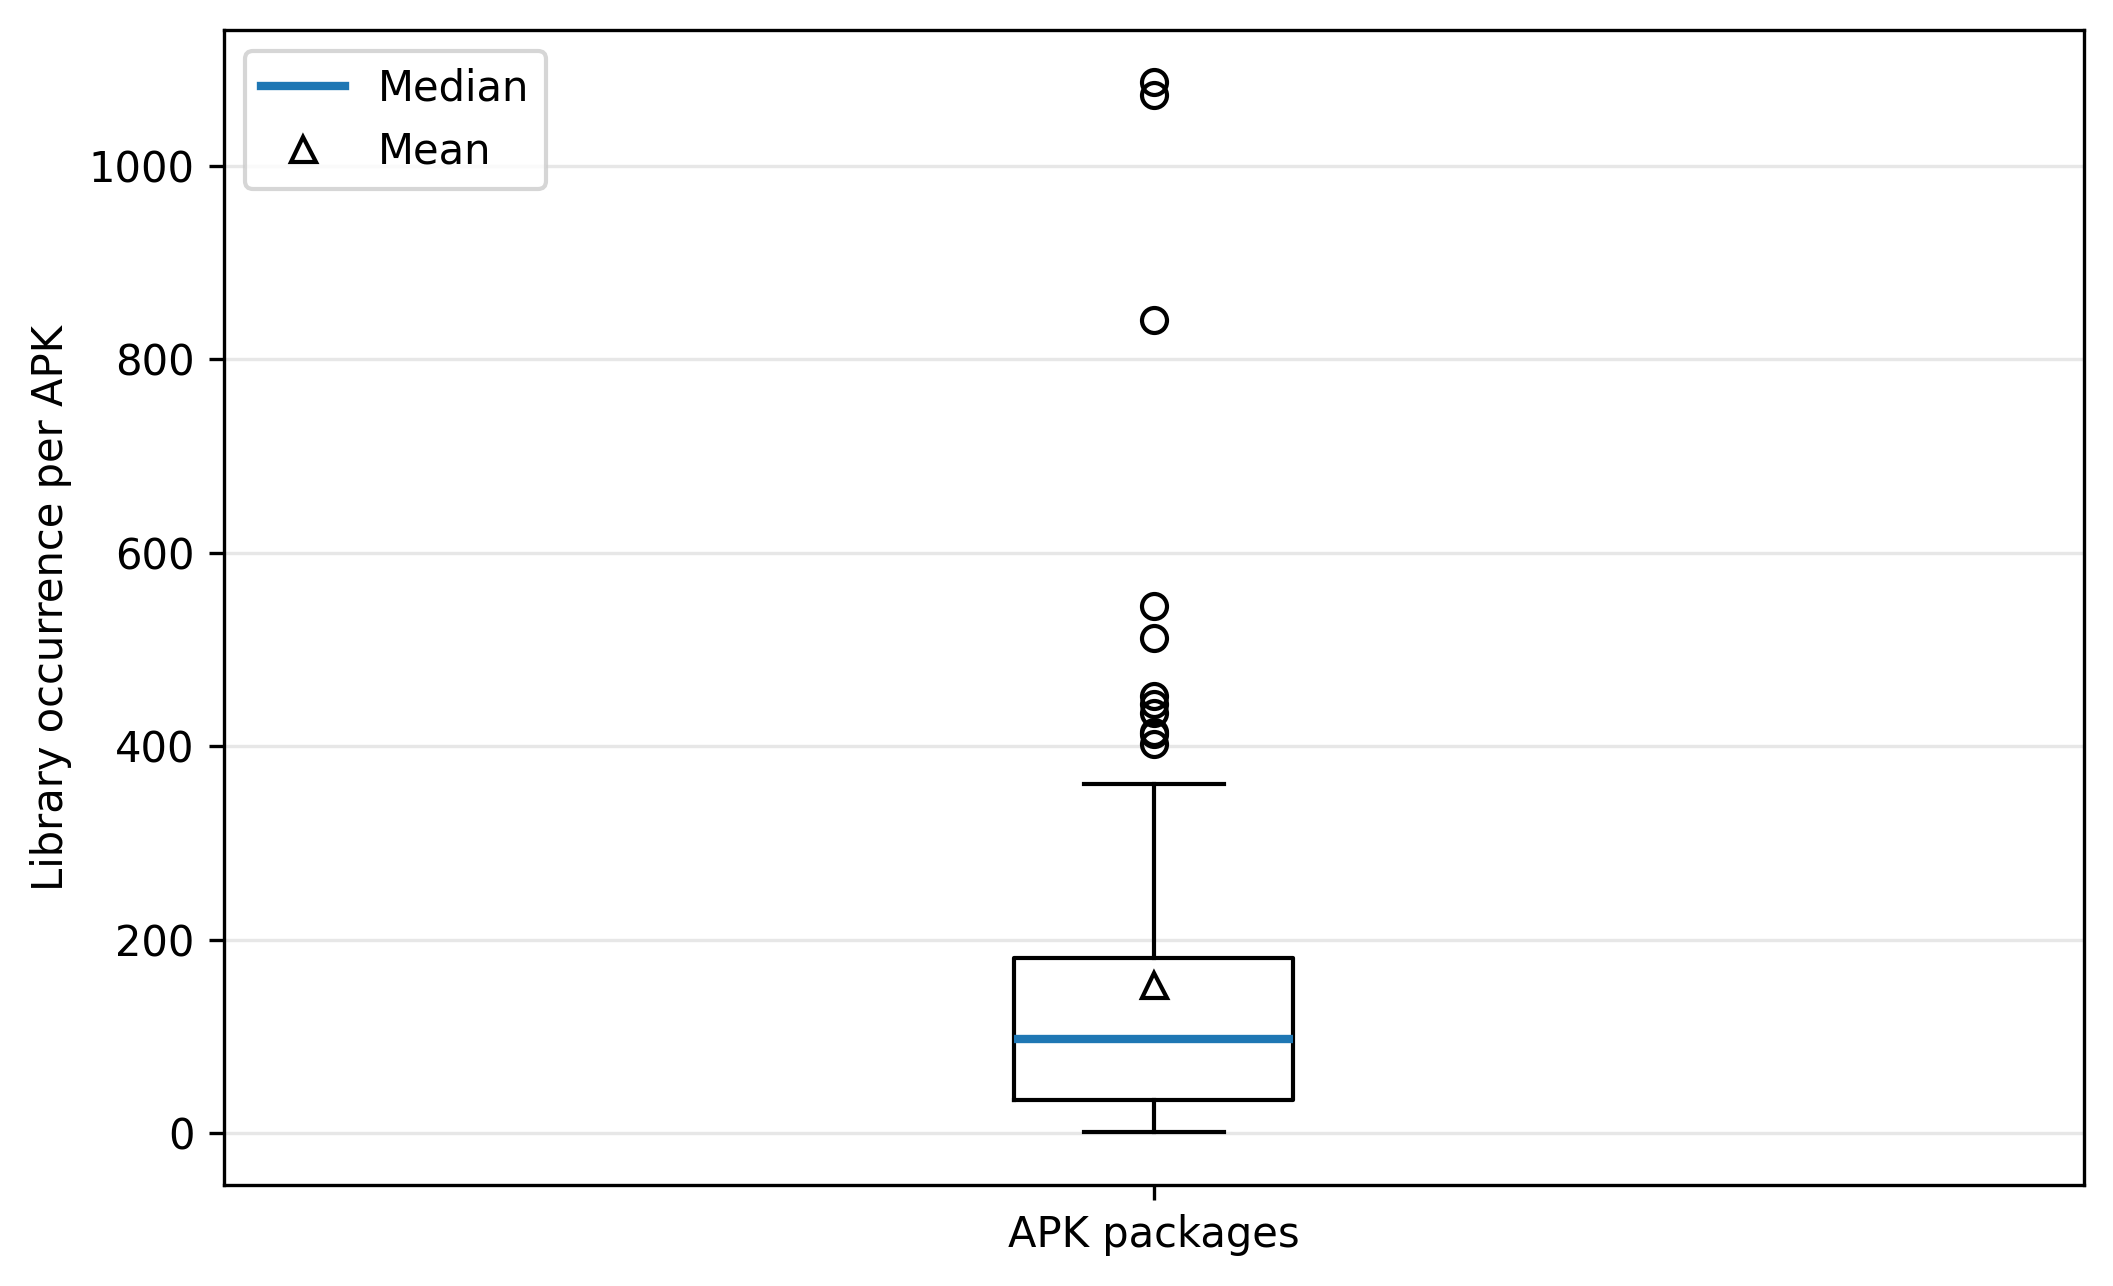
\includegraphics[width=0.7\textwidth,keepaspectratio]{image/library_occurrences_per_apk_boxplot_fdroid.png}
\caption{Distribution of detected library occurrences per APK in the F-Droid validation set}
\label{fig:library-occurrences-per-apk-fdroid}
\end{figure}

\section{Source-Code Library Extraction Methods}
The source-code validation step uses an extendable detector structure. Each method scans the cloned repository in a different way and contributes candidate library declarations. At this stage, five source-code detection methods are used:

\begin{enumerate}
\item \textbf{Gradle dependency detection}: scans \texttt{build.gradle} and \texttt{build.gradle.kts} files for dependency declarations such as \texttt{implementation}, \texttt{api}, \texttt{compileOnly}, \texttt{runtimeOnly}, \texttt{kapt}, and test-related configurations.
\item \textbf{Version catalog detection}: scans \texttt{libs.versions.toml} files and extracts entries from the \texttt{[libraries]} section.
\item \textbf{Third-party markup detection}: scans documentation files in directories such as \texttt{thirdparty}, \texttt{third\_party}, and \texttt{vendor}, including cases where libraries are listed in markup notes (README and LICENSE).
\item \textbf{Vendor directory detection}: scans common bundled-library directories such as \texttt{thirdparty}, \texttt{third\_party}, \texttt{vendor}, \texttt{external}, and \texttt{libs}, and records subdirectories as possible embedded libraries.
\item \textbf{GitHub URL detection}: scans text-like files across the repository for GitHub repository URLs and records them as candidate third-party libraries. Links pointing to the application repository itself are excluded so that internal project references are not counted as external libraries.
\end{enumerate}

\section{Matching APK Findings Against Source-Code Findings}
The matching process uses \texttt{pkg\_name} as the first-level identifier. This means that a library detected in an APK is only compared with source-code libraries extracted from the corresponding application's repository. Within each package, the second-level matching uses multiple identifiers: \texttt{library\_key}, \texttt{library\_name}, Gradle coordinates, repository path, repository URL, and extracted GitHub URLs.

Because the APK-derived dataset and source-code-derived dataset do not always describe the same library in the same format, exact matching alone would be too strict. Therefore, the comparison uses several partial matching methods:

\begin{enumerate}
\item \textbf{Repository URL matching}: compares normalized repository URLs and repository paths, including partial matches such as \texttt{owner/repo} appearing inside a longer URL.
\item \textbf{Namespace matching}: checks whether one normalized library key or library name appears inside the other. For example, \texttt{okhttp} may match \texttt{com.squareup.okhttp3:okhttp}.
\item \textbf{Artifact matching}: extracts the artifact part from Gradle coordinates or repository paths and compares this shorter identifier.
\end{enumerate}

\section{Validation Results on the F-Droid Control Set}
The validation produced the following matching results for the 100 F-Droid applications:

\begin{itemize}
\item Matched source-code rows: \textbf{2,741}
\item Matched APK rows: \textbf{11,740}
\item Total match relationships: \textbf{106,197}
\end{itemize}

The match relationships were distributed across the matching methods as follows:

\begin{table}[htbp]
\centering
\caption{Distribution of match types in the F-Droid validation set}
\label{tab:fdroid-validation-match-types}
\begin{tabular}{lr}
\hline
\textbf{Match type} & \textbf{Number of match relationships} \\
\hline
Contains match & 63,810 \\
Artifact match & 28,108 \\
Repository URL match & 14,279 \\
\hline
\textbf{Total} & \textbf{106,197} \\
\hline
\end{tabular}
\end{table}

Using the source-code analysis as the approximate ground truth, the APK analysis achieved the following validation metrics:

\begin{table}[htbp]
\centering
\caption{Validation metrics using source-code analysis as approximate ground truth}
\label{tab:fdroid-validation-accuracy}
\begin{tabular}{lr}
\hline
\textbf{Metric} & \textbf{Value} \\
\hline
True positive matched source rows & 2,741 \\
False negative source rows missed by APK analysis & 3,738 \\
False positive APK rows not supported by source analysis & 3,613 \\
Recall / ground-truth coverage & 42.31\% \\
Precision / APK supported by source & 43.14\% \\
F1 score & 42.72\% \\
\hline
\end{tabular}
\end{table}

These results show that the validation baseline is more informative than the original manual in-app emulator inspection. The recall value indicates that the APK pipeline identifies a meaningful portion of source-code-derived dependency evidence, but also misses a substantial number of libraries visible in the source-code analysis. The precision value shows that many APK-detected rows are not directly confirmed by the current source-code extraction method. This does not automatically mean that all of these rows are false positives. Source-code dependency extraction is itself incomplete and may miss generated dependencies, bundled code, build-time transformations, or libraries introduced through external build logic. In addition, part of the 3,613 APK rows not confirmed by source-code evidence may represent transitive dependencies present in the compiled APK rather than explicitly declared direct dependencies in the scanned source-code files.

\section{Limitations of Validation}
The validation should be interpreted as an approximate baseline rather than a perfect ground truth. Source code provides stronger evidence than in-app license screens, but static source-code scanning may still miss conditional dependencies, build variants, aliases, generated code, bundled binaries, and dependencies introduced through external build logic. Conversely, the compiled APK may contain libraries that are not clearly visible in the scanned source branch, including transitive dependencies or build-time additions.

The matching logic is intentionally permissive because APK evidence and source-code declarations often use different identifiers. Partial matching improves coverage, but it can also introduce false matches. A more exact validation would require opening each project in Android Studio and manually inspecting the full build configuration and codebase. Increasing the corpus size and fingerprint database may also change the accuracy in both directions: it can improve detection by discovering more libraries, but it can also introduce more transitive APK libraries that are difficult to match back to explicit source-code declarations. Therefore, the validation results should be read as a practical performance baseline for the current pipeline, not as a final measurement of absolute correctness.


\chapter{Results and Discussion}
\section{Findings}
In this section, we will see the empirical findings derived from the APK-level analysis, focusing on library detection, citation behavior, and dependency structure. The results are based on the output dataset generated by the pipeline for the 699 APK corpus size.

\subsection{Summary of Key Performance Indicators (KPIs)}
The analysis of the APK corpus reveals consistent patterns in open-source library usage. The following KPIs summarize the main characteristics of the dataset:

\begin{itemize}
\item Average number of libraries per APK: \textbf{154.84}
\item Total number of unique libraries across corpus: \textbf{636}
\item Ratio of declared (cited) libraries: \textbf{55.39\%}
\item Ratio of undeclared libraries: \textbf{44.61\%}
\item Ratio of library records supported by fingerprint-based evidence: \textbf{96.06\%}
\item Total library occurrence rows (evidence instances): \textbf{108,234}
\end{itemize}

These indicators suggest that Android applications rely heavily on external libraries, with an average of 154.84 library occurrences per APK. At the same time, only 55.39\% of detected libraries are explicitly declared through license information, while 44.61\% are identified exclusively through fingerprint-based detection. This demonstrates a substantial gap between actual dependency usage and documented license disclosure.

The high fingerprint-based evidence ratio (96.06\%) shows that the fingerprint method delivers the expected result and can identify most library usage through code evidence. This is also computationally important because fingerprint lookup is less costly than full license-exposure lookup. The license-exposure check is therefore used mainly in the final stage to revalidate whether detected libraries are actually cited, and the results show that many are not. The detection-origin distribution for the 699 APK corpus is shown in Appendix Figure~\ref{fig:fingerprints-vs-license-exposure-apk-700} (Also look at the full summary at Appendix Table~\ref{tab:summary-kpis-final-corpus}).


\subsection{Library Detection and Citation Behavior}
One of the most important findings of the analysis is the discrepancy between detected libraries and declared licenses. Out of 108,234 detected library occurrences, 48,280 instances (44.61\%) were identified only through fingerprint matching, indicating that license declarations are frequently incomplete or absent (Figure~\ref{fig:cited-vs-uncited}). There is no pattern in the app categories.


\begin{figure}[htbp]
\centering
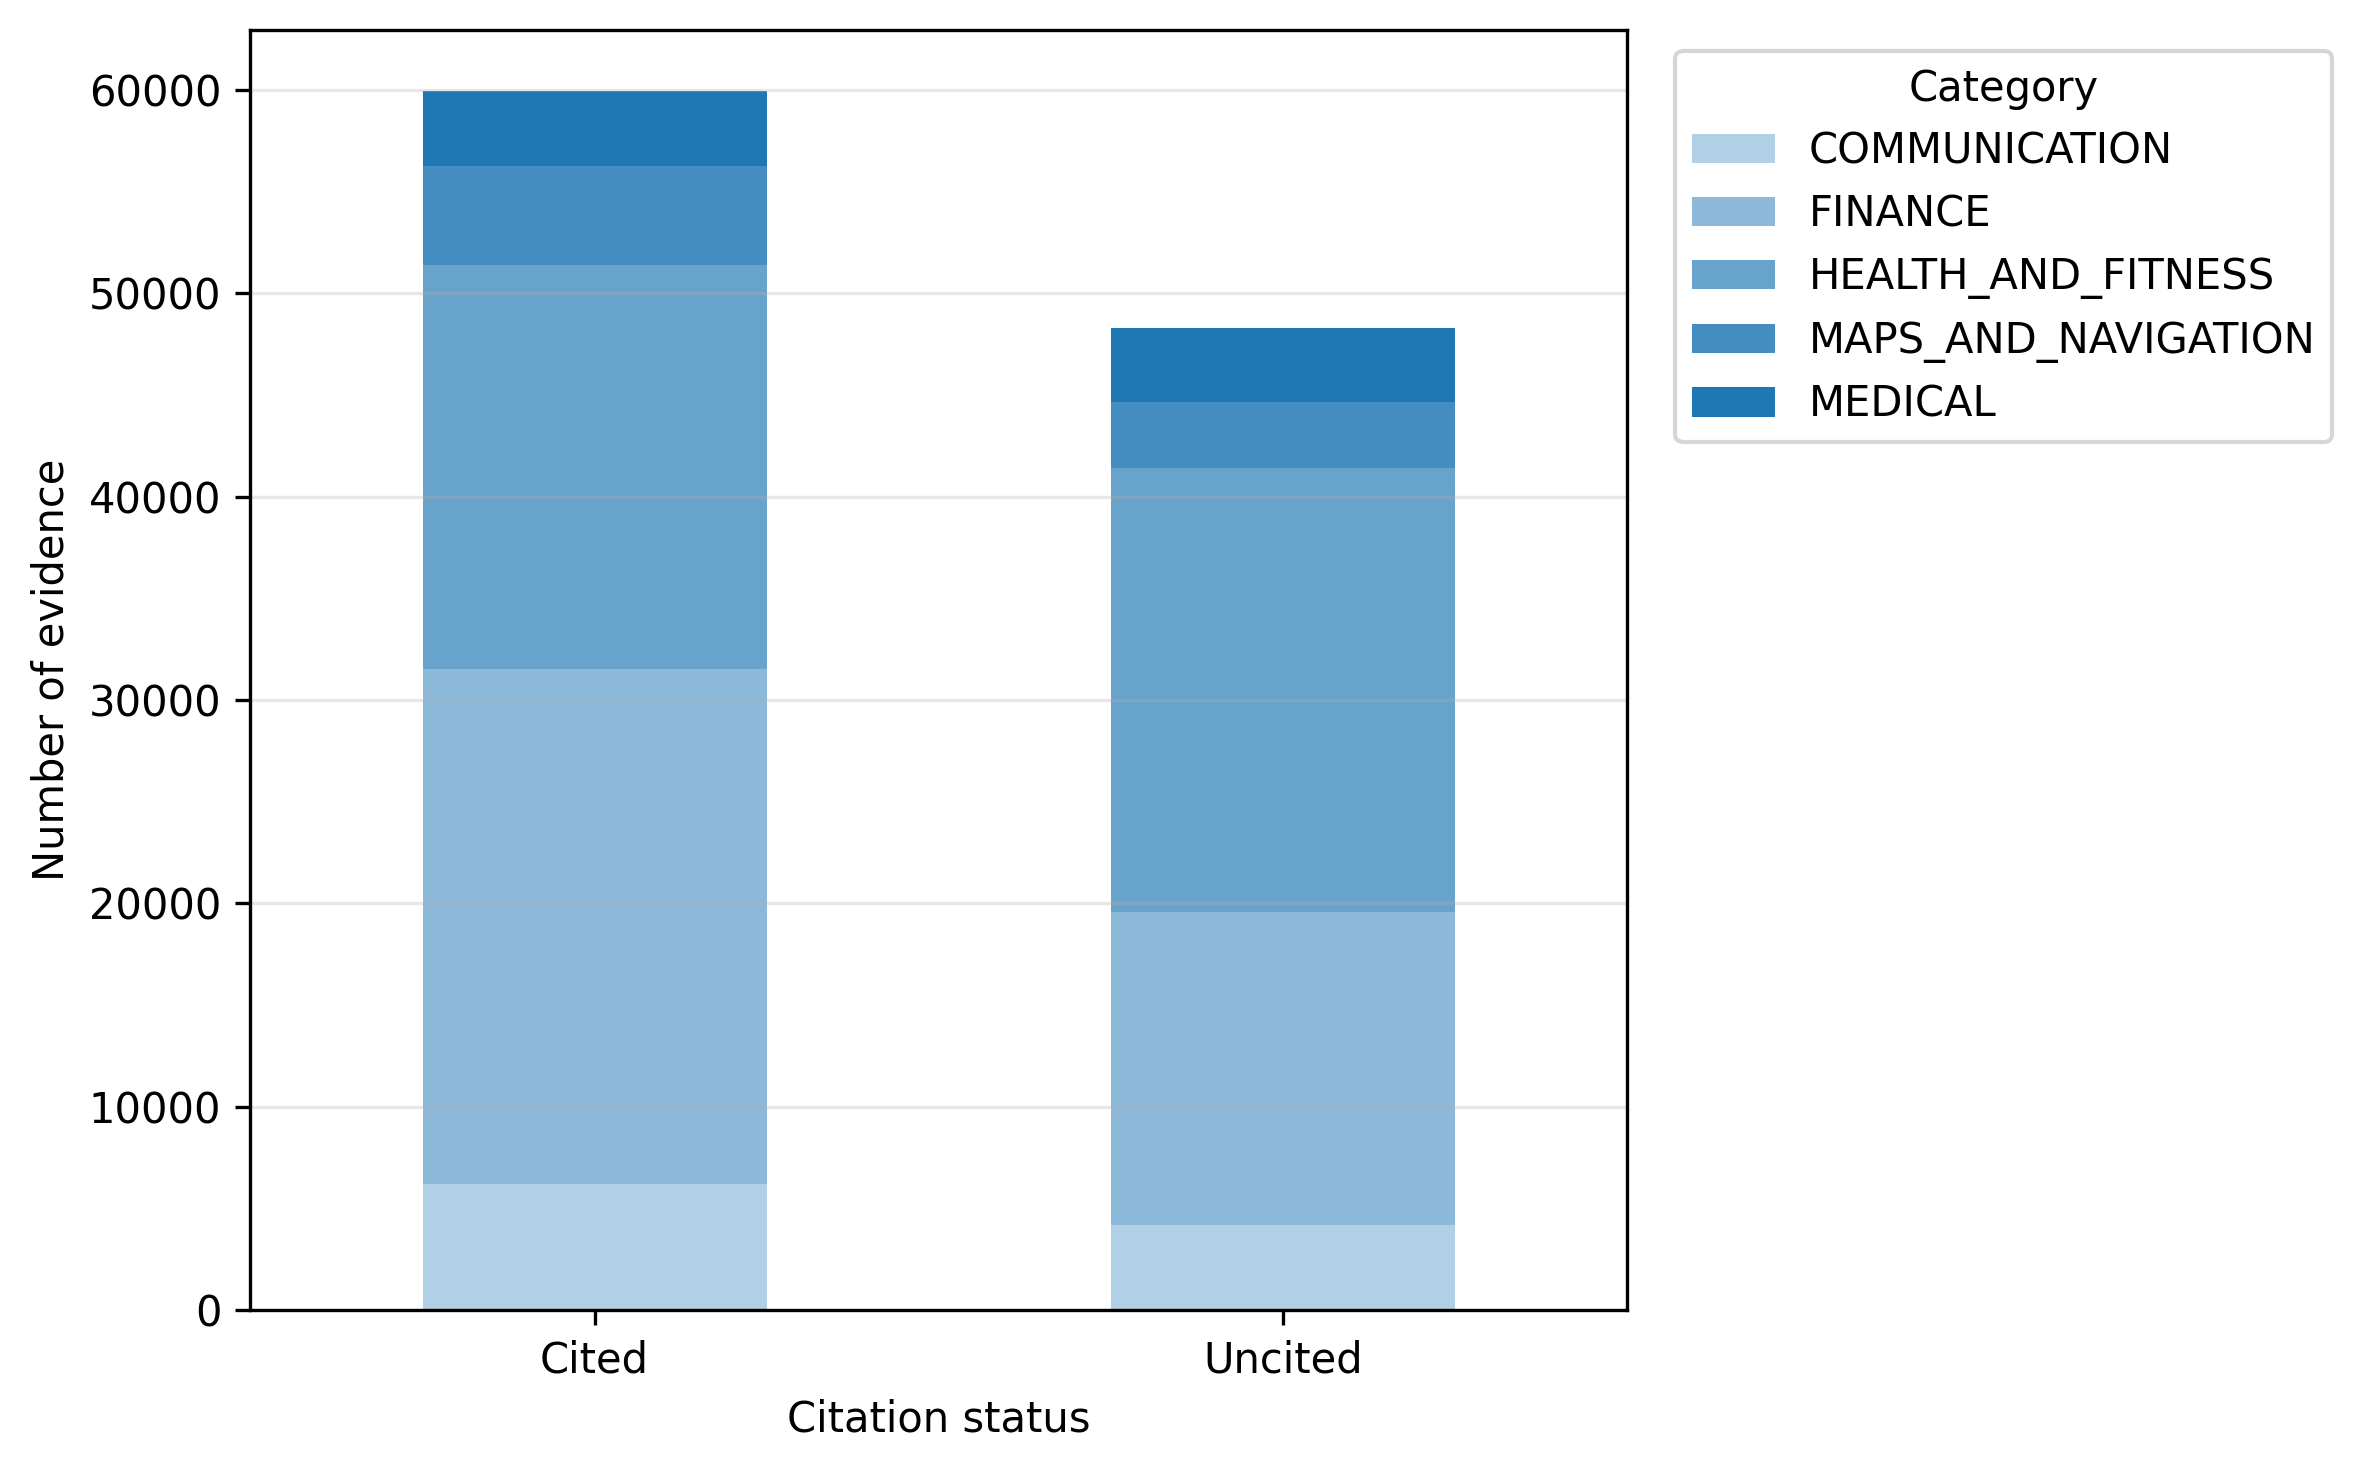
\includegraphics[width=0.7\textwidth,keepaspectratio]{image/cited_vs_uncited_by_category.png}
\caption{Distribution of cited versus uncited libraries}
\label{fig:cited-vs-uncited}
\end{figure}

\subsection{Distribution of Libraries Across APKs}
The distribution of libraries per application shows high variability. As shown in Figure~\ref{fig:lib-dist-per-apk}, the mean number of detected library occurrences per APK is 154.84, while the median is lower at 123, indicating that some applications contain much larger dependency sets. In the final corpus, 55 APKs have fewer than 10 detected libraries, whereas 52 APKs have more than 400 detected libraries (For detailed info look at Appendix Figure~\ref{fig:library-occurrences-per-apk-histogram} and Figure~\ref{fig:fingerprints-vs-license-exposure-apk-700}.)

\begin{figure}[htbp]
\centering
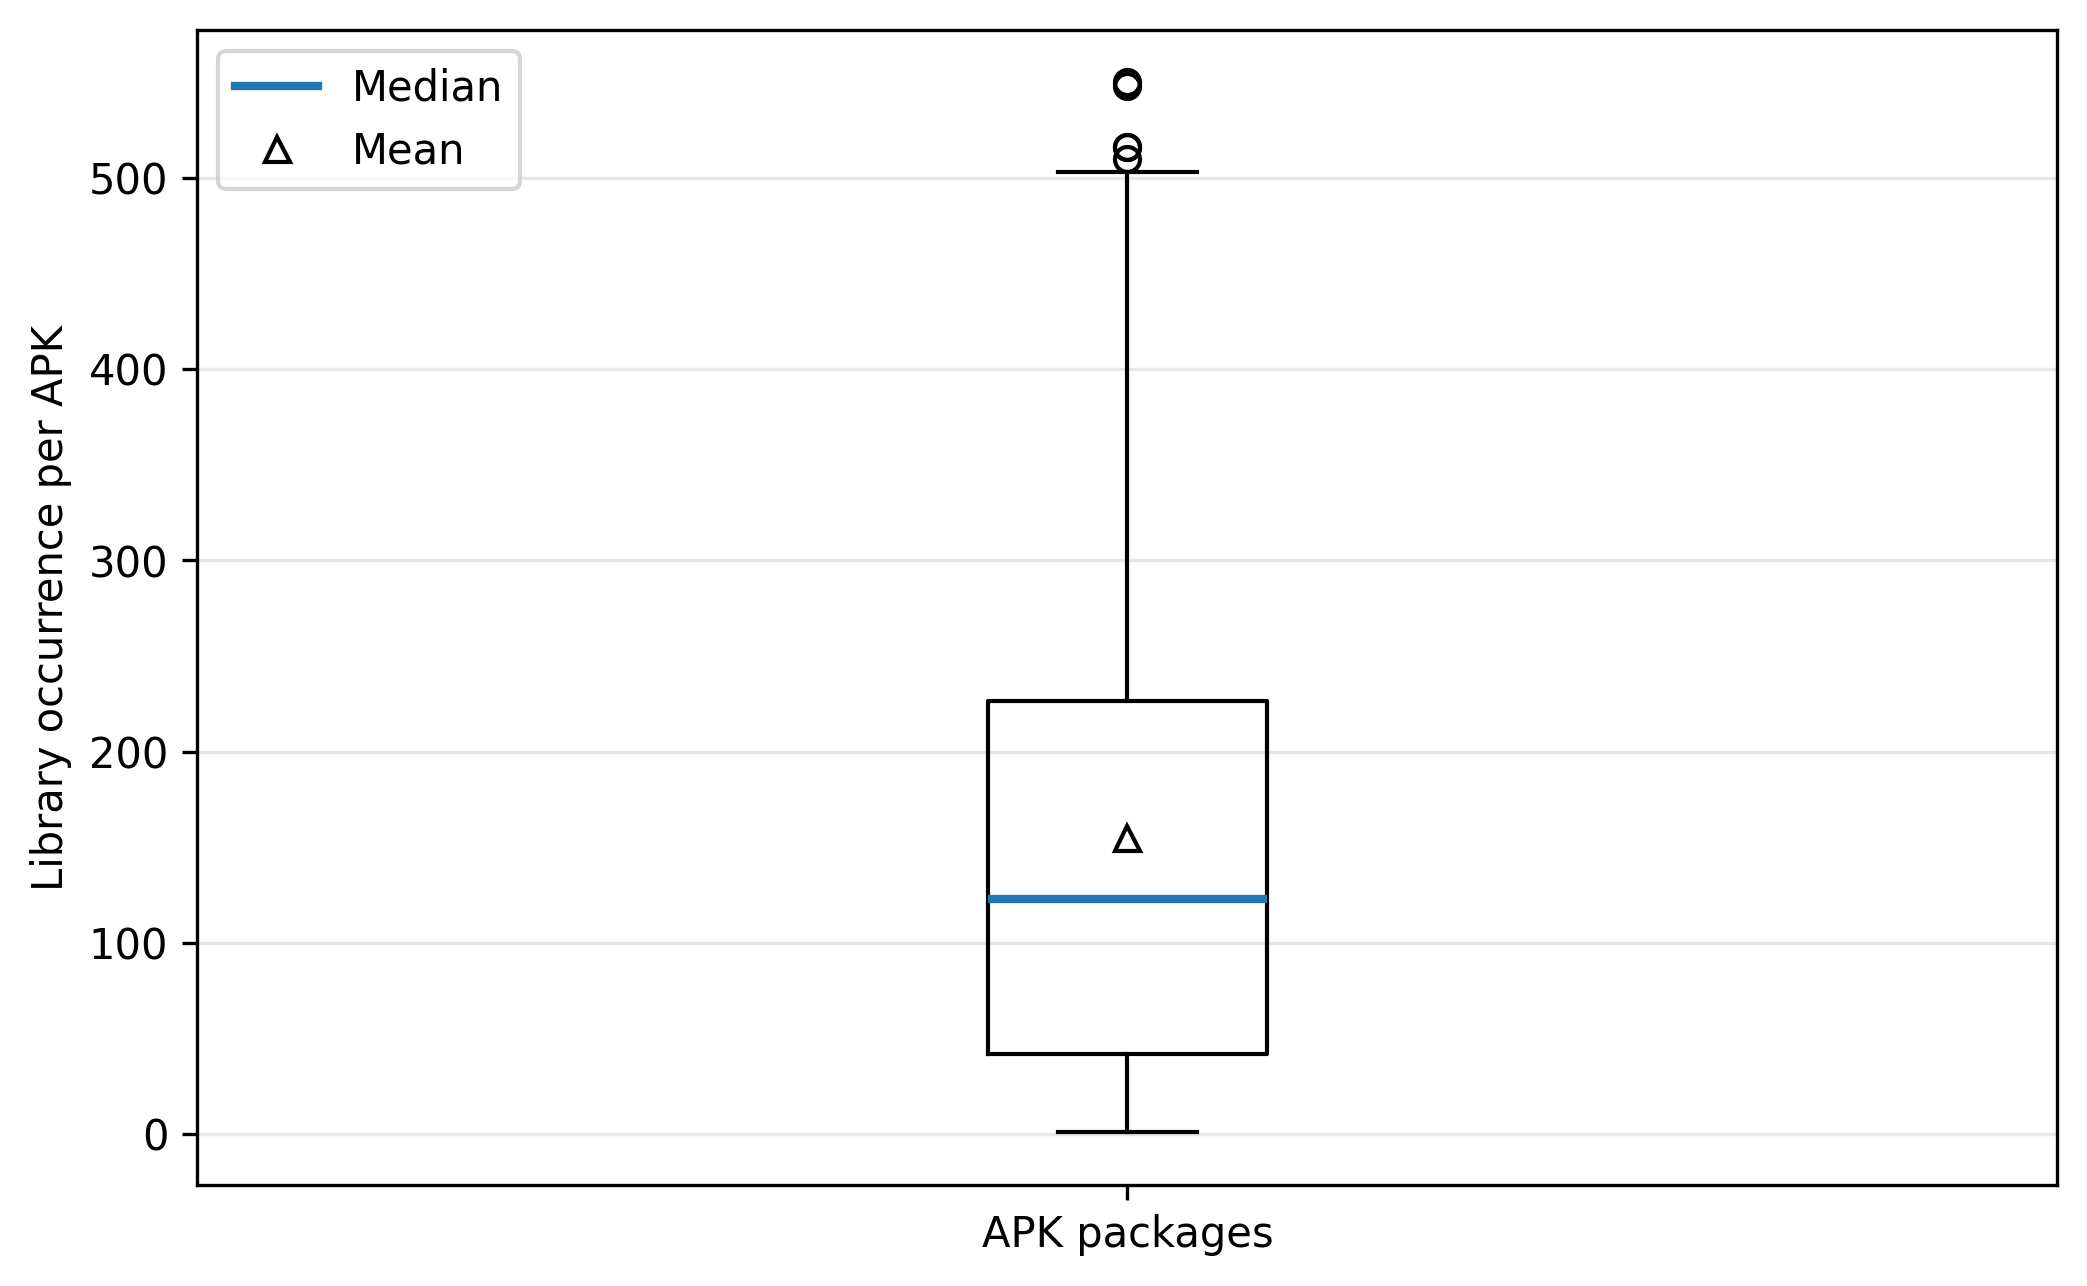
\includegraphics[width=0.7\textwidth,keepaspectratio]{image/library_occurrences_per_apk_boxplot.png}
\caption{Distribution of detected library occurrences per APK}
\label{fig:lib-dist-per-apk}
\end{figure}

The APK-level results show that dependency usage in Android applications is both extensive and partially hidden.

\subsection{Medium-Health Level Open Source Library Usage in APKs}\label{sec:medium-health-level-open-source-library-usage-in-apks}
After the APK-level analysis, the repository-level Wang and Wu health scores were joined back to the APK/library evidence dataset. This makes it possible to identify which applications use libraries classified as having \textit{medium} repository health and to measure how intensely those libraries appear inside each APK. In this analysis, usage intensity is measured through \texttt{classes\_matched}, which is used as a proxy for how strongly a detected library appears in the decoded APK codebase.

Across the largest analyzed corpus, the dataset contains \textbf{108,234} APK/library evidence rows. Of these, \textbf{98,330} rows could be joined to a GitHub repository with an assigned health level. Within this joined dataset, \textbf{225} rows correspond to libraries classified as \textit{medium health}. These medium-health rows appear at least one time in \textbf{89} distinct APKs. This means that medium-health libraries are not limited to isolated cases; they appear across a \textbf{12.7\%} of the analyzed application corpus size.

\subsubsection{How intense is medium-health library use inside each APK?}
The intensity of medium-health library usage is calculated as the share of class matches associated with medium-health libraries relative to all detected open-source class matches in the same APK:

\begin{equation}
MediumHealthIntensity = \frac{medium\_health\_classes\_matched}{apk\_total\_classes\_matched} \times 100
\end{equation}

This measure does not claim to represent runtime execution frequency. Instead, it captures how much of the detected open-source code evidence inside an APK is associated with repositories classified as medium health. Applications with high values should therefore be interpreted as having stronger structural exposure to medium-health libraries.

\subsubsection{Which APKs use open-source libraries with medium health?}
The first question is which APKs contain at least one open-source library classified as \textit{medium health}. The analysis identifies \textbf{89} such APKs. For each APK, the aggregation records the number of medium-health evidence rows, the number of unique medium-health repositories, the number of matched classes associated with these libraries, and the percentage of the APK's total detected open-source class matches represented by medium-health libraries.

The ranking is based on intensity of medium-health library use (\texttt{medium\_health\_intensity\_pct\_of\_apk}). The highest observed values include \textit{KidiCom Chat™ (FR)} at \textbf{18.75\%}, \textit{CEMAH netCEM} at \textbf{1.71\%}, and \textit{NeurOm} at \textbf{0.57\%} (Figure~\ref{fig:top-apks-medium-health-intensity}). These applications therefore show the strongest relative presence of medium-health libraries within their detected open-source class usage.


\begin{figure}[htbp]
    \centering
    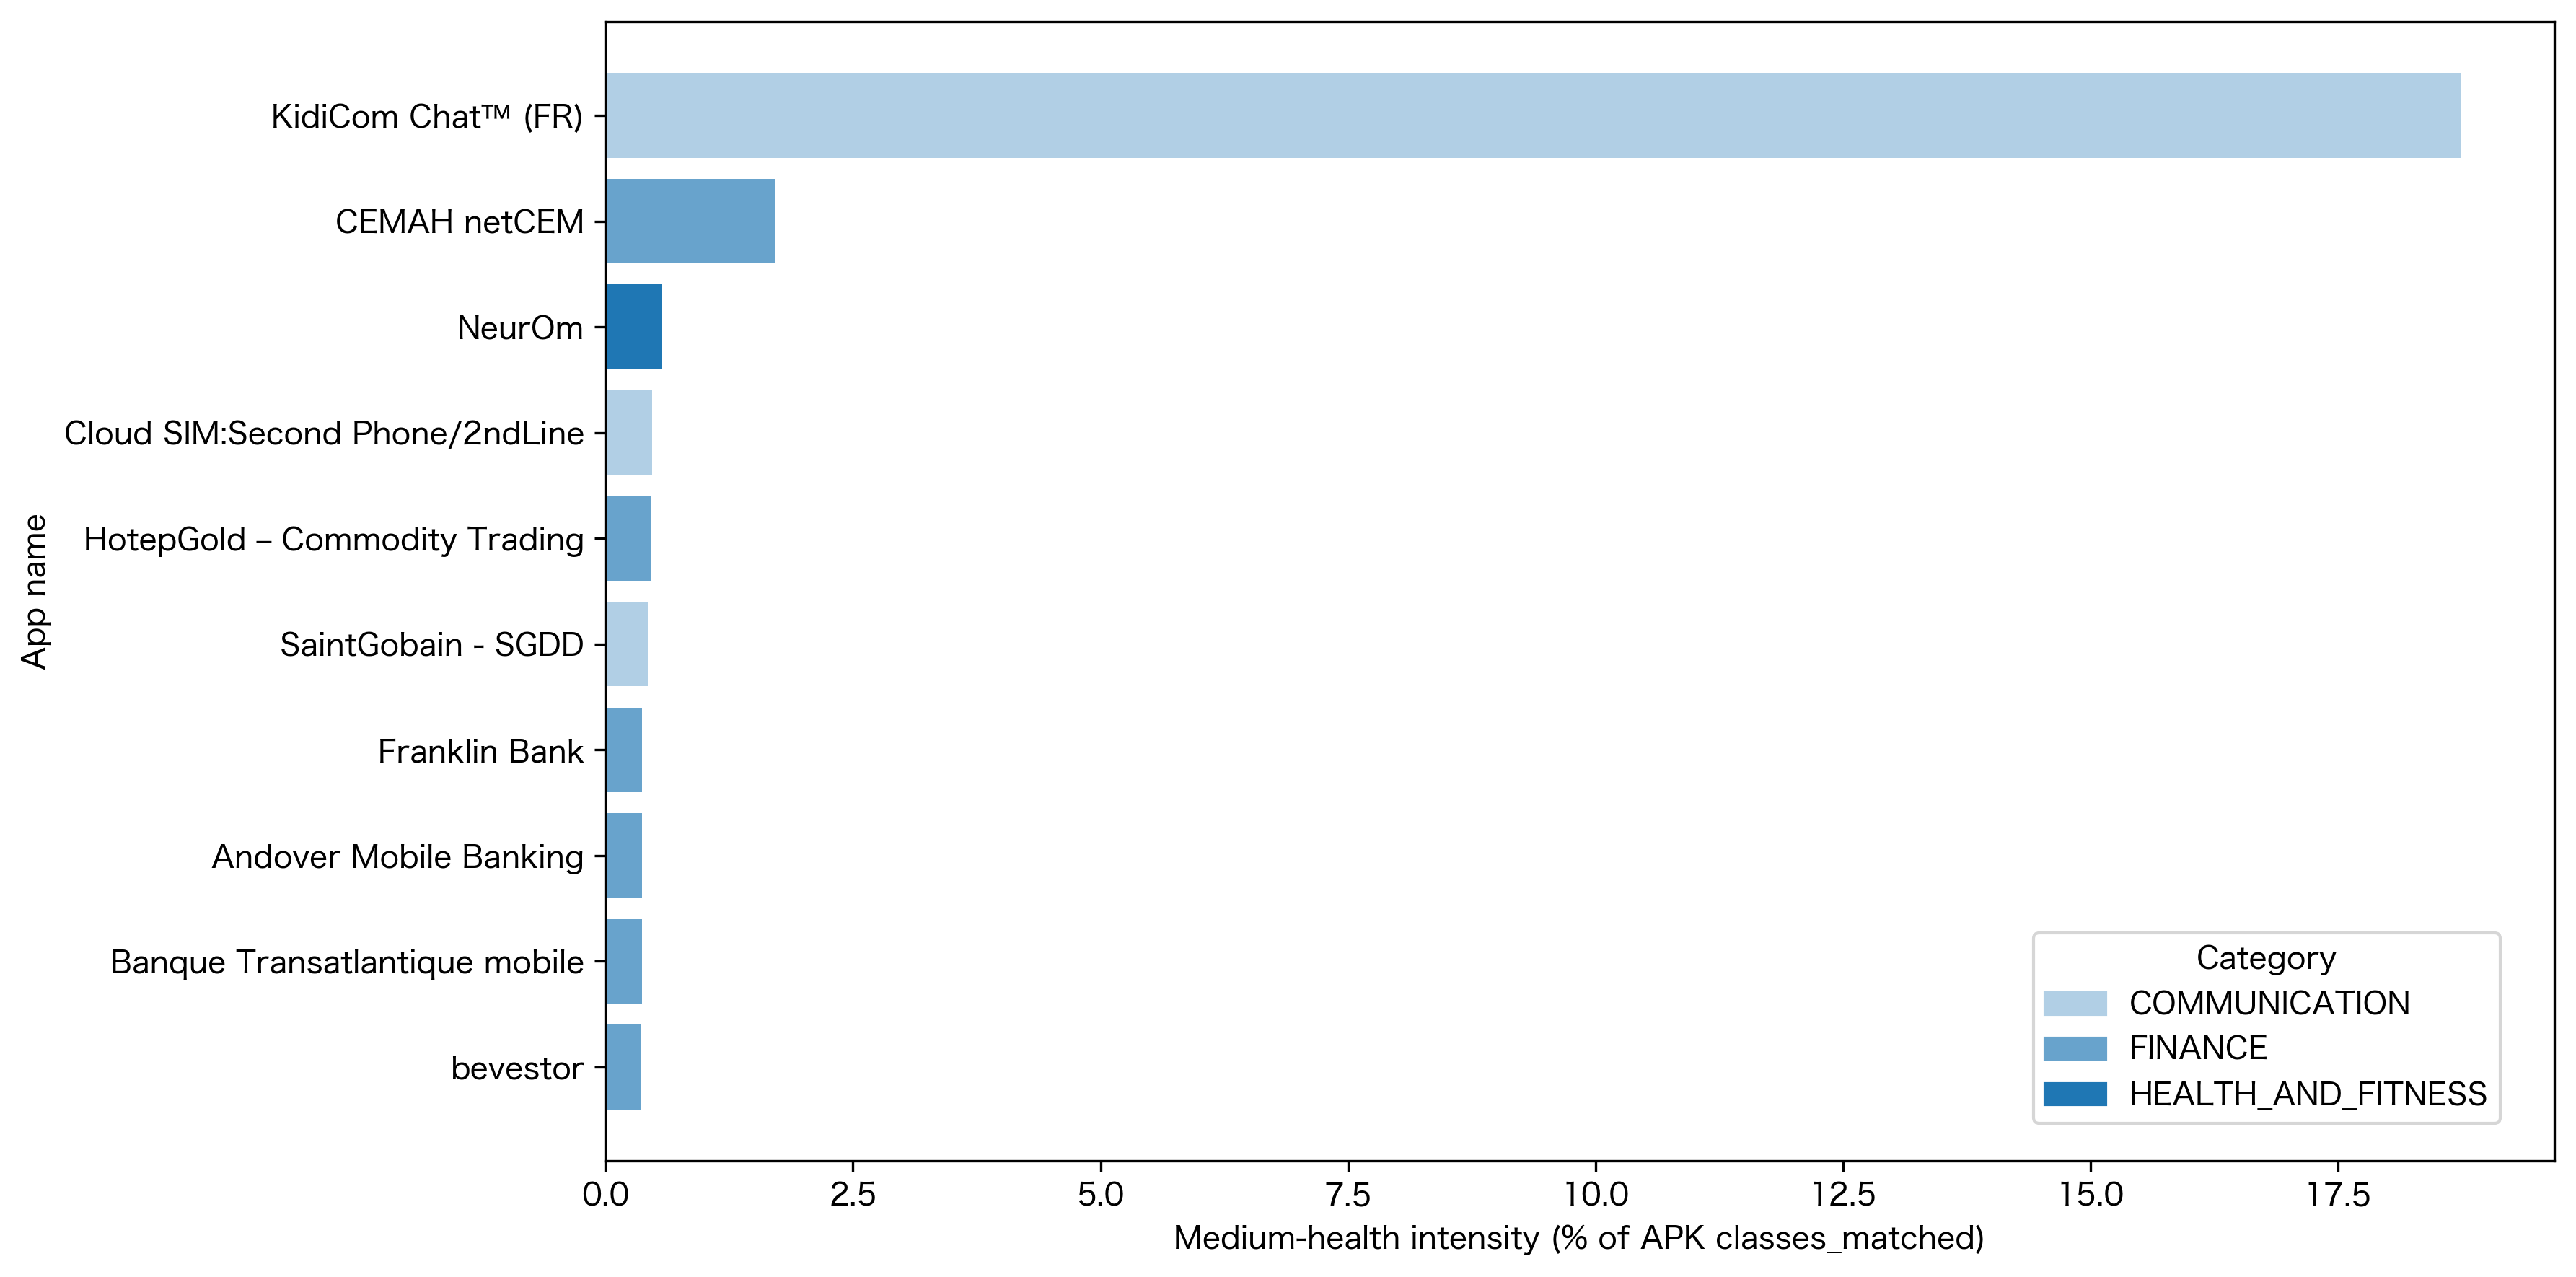
\includegraphics[width=\textwidth,keepaspectratio]{image/top_apps_by_medium_health_intensity.png}
    \caption{Top 10 APKs by medium-health library usage intensity}
    \label{fig:top-apks-medium-health-intensity}
    \end{figure}

\subsubsection{Which APKs use medium-health libraries but uncited (cited = 0)?}
The second part of the analysis focuses only on medium-health rows where \texttt{cited = 0}. These are cases where the pipeline found code evidence of a medium-health library, but no corresponding license declaration was identified in the APK evidence. The dataset contains \textbf{69} uncited medium-health rows, appearing across \textbf{34} distinct APKs.

The leading APKs by uncited medium-health library use intensity include \textit{HotepGold – Commodity Trading}, \textit{bevestor}, and \textit{Dubai Bus on Demand} (Figure~\ref{fig:top-apks-uncited-medium-health-intensity}). These cases are important because the relevant medium-health libraries are detected through code evidence but are not visible through license citation. As a result, even a technically skilled user would have little practical opportunity to identify these libraries from the APK disclosure information alone and react if one of them became risky.

\begin{figure}[htbp]
\centering
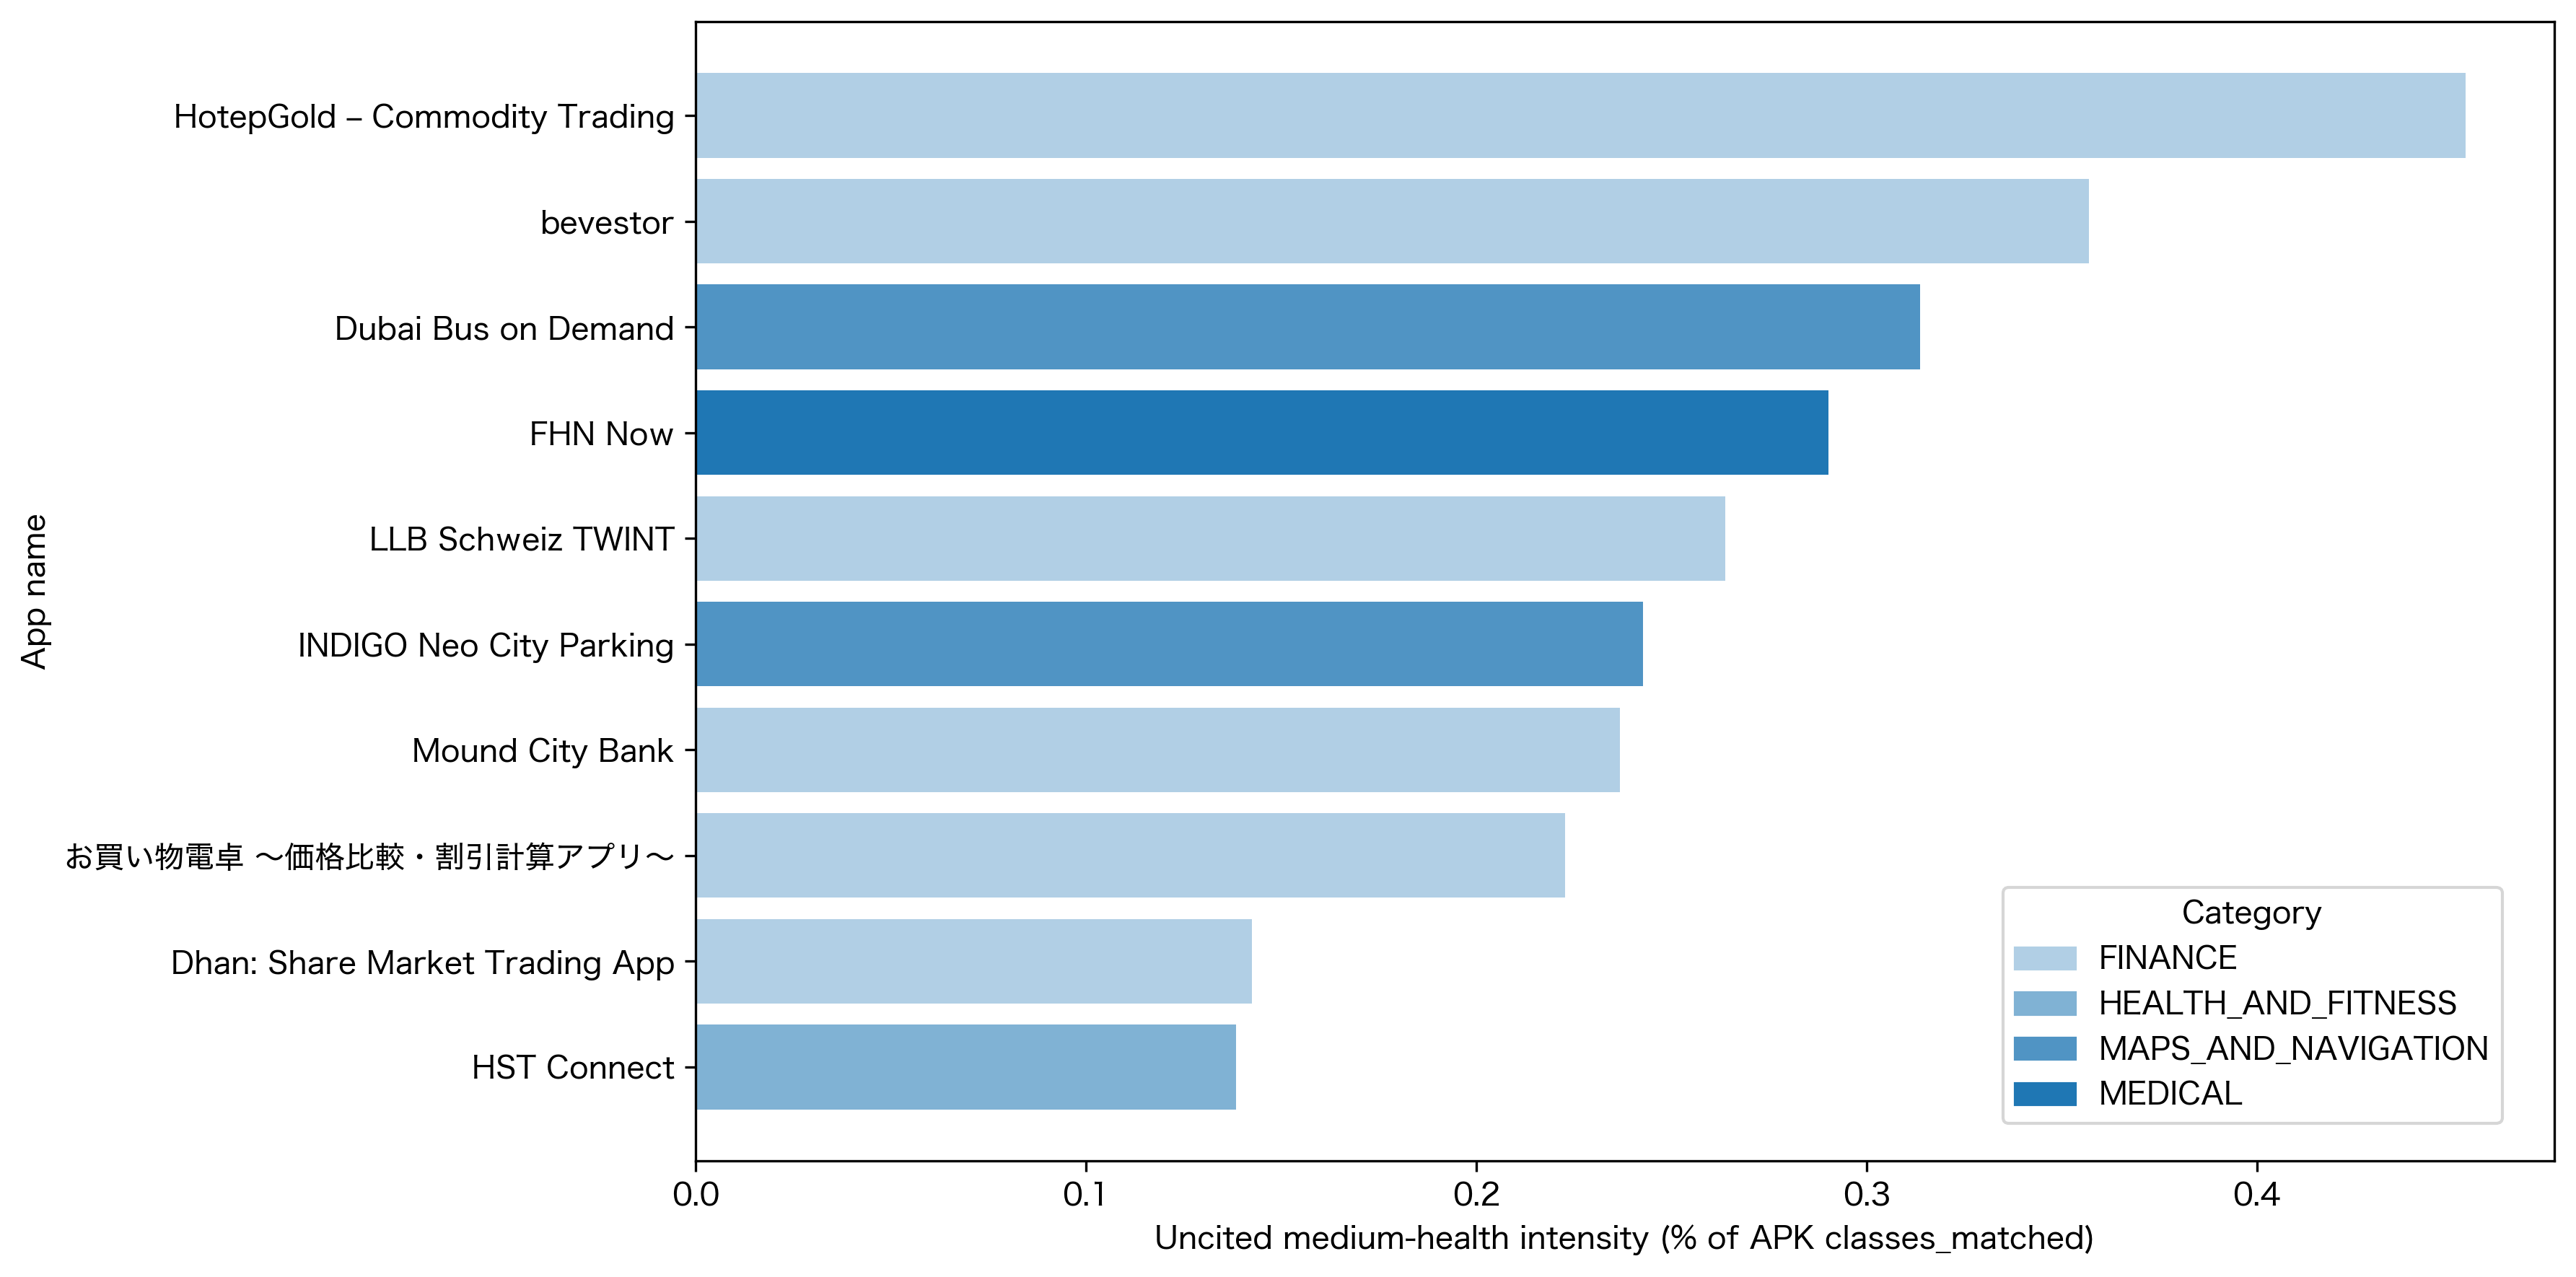
\includegraphics[width=\textwidth,keepaspectratio]{image/top_apps_by_uncited_medium_health_intensity.png}
\caption{Top 10 APKs by uncited medium-health library usage intensity}
\label{fig:top-apks-uncited-medium-health-intensity}
\end{figure}


\section{Interpretation of Results}
From these findings, we can draw the following main interpretations:

\begin{itemize}
\item Android applications in the corpus rely heavily on external open-source libraries, with an average of 154.84 detected library occurrences per APK.
\item License disclosure is incomplete: 44.61\% of detected library occurrences are uncited, meaning they are found through code evidence but not through license declarations.
\item The fingerprint-based method is effective for this research goal, because 96.06\% of cited library records are also confirmed by fingerprint evidence.
\item Dependency usage varies widely across applications, from APKs with very few detected libraries to APKs with more than 400 library occurrences.
\item Repository-level analysis shows that, among the 220 repositories with assigned Wang and Wu health levels, 204 are classified as high health and 16 as medium health, while no repository falls into the low-health category.
\item Medium-health libraries appear in 225 APK/library evidence rows across 89 distinct APKs, representing 12.7\% of the analyzed application corpus.
\item Uncited medium-health libraries are especially important because users and auditors cannot easily identify them from license disclosure alone; in this corpus, 69 uncited medium-health rows appear across 34 APKs.
\end{itemize}

Overall, the results show that the main issue is not only the presence of open-source libraries, but the gap between actual library usage and what is disclosed to users or reviewers. The repository-health analysis adds another layer to this finding by showing which detected libraries come from repositories with lower health levels.

\section{Implications for Developers}
The findings show that many libraries are present in APK code but are not visible through license declarations. Developers should therefore make dependency visibility and license declaration part of the CI/CD process, not a final manual documentation step. Software composition analysis, SBOM-style documentation, fingerprint-based checks, and repository-health monitoring can help teams verify which libraries are actually embedded in their applications and reduce the gap between used and declared dependencies.

\section{Implications for End Users}
As end users, we face limited transparency. Because many libraries are uncited, we cannot realistically identify which dependencies an app contains, whether they are secure, or whether they are actively maintained. This is especially important for apps in sensitive categories such as finance, health, communication, and navigation. Since we have almost no practical way to evaluate hidden dependencies, uninstalling unused apps in these categories is a reasonable risk-reduction practice.

\chapter{Conclusion}
\section{Answer to Research Questions}
We can now return to the research questions and answer them based on the results. The thesis investigated whether external open-source libraries can be detected in compiled Android APK files and whether the detected dependencies are consistently disclosed through license information. The results show that fingerprint-based evidence can reveal substantial library usage that is not visible from license declarations alone.

\textbf{RQ1: Is it feasible to detect external libraries in Android APK files?}
Yes. The developed pipeline successfully processed the APK corpus, decoded applications, extracted license evidence, generated fingerprints from source repositories, and matched those fingerprints against decoded APK code. In the final corpus, the pipeline produced 108,234 library occurrence rows across 699 APKs, showing that automated library detection is feasible at this scale.

\textbf{RQ2: How reliable are license declarations and package fingerprints for identifying library dependencies?}
License declarations are useful but incomplete. In the final corpus, only 55.39\% of detected library occurrences were cited, while 44.61\% were uncited and visible only through code evidence. Package fingerprints were more effective for detection: 96.06\% of cited library records were also confirmed by fingerprint evidence. This supports the use of fingerprints as the main detection method, with license exposure used mainly for citation validation.

\textbf{RQ3: How many open-source libraries, and what types of them, are used in a sample of Android applications?}
The final corpus contains 636 unique repository URLs and an average of 154.84 detected library occurrences per APK. The libraries are mainly detected through Java and Kotlin package fingerprints. Repository-level analysis also showed that among the 220 GitHub repositories with assigned health levels, 204 repositories were classified as high health, 16 repositories were classified as medium health, and no repository was classified as low health.

\textbf{RQ4: Which Android applications show the highest dependency on low-health or medium-health open-source libraries?}
The analysis identified 225 medium-health APK/library evidence rows across 89 distinct APKs and it doesn't identify any low-health libraries. Dependency strength was measured by medium-health library use intensity, meaning the percentage of an APK's total detected open-source class matches that belong to medium-health repositories. Based on this intensity measure, the leading applications are \textit{KidiCom Chat™ (FR)}, \textit{CEMAH netCEM}, and \textit{NeurOm}. These applications therefore have the strongest relative exposure to medium-health libraries within their detected open-source code evidence.

Overall, the practical part of the thesis was applicable and completed: the APK collection was built, the decoding and matching pipeline was implemented, GitHub metadata was collected, repository health scores were calculated, and the final dataset was analyzed. The pipeline can also target a standalone APK, add it to the corpus, identify its open-source library ingredients, assess their repository health levels, and compare it with other APKs. The validation chapter showed that in-app license screens are usually not a reliable validation baseline, while the F-Droid source-code control set provided a more useful approximate ground truth and confirmed that the pipeline can recover a meaningful portion of dependency evidence, although both precision and recall remain limited by differences between compiled APK contents and source-code declarations.

Some expectations were only partially achieved. The corpus size remained limited by hardware and lookup time, the sample was not category-balanced, manual validation was limited because most applications did not expose in-app license information, and the method cannot prove runtime execution of a library. Therefore, the results should be interpreted as evidence of embedded library presence, repository-health context, and disclosure gaps, not as a complete runtime security assessment.

\section{Future Work}
The pipeline created a labeled corpus that records which files and lines contain evidence of external library imports, exports, and class references. This creates an opportunity for future work based on text analysis and machine learning. Instead of relying only on rule-based fingerprint matching and repeated lookup operations, future versions of the system could tokenize the indexed evidence lines and train a model to classify whether a line is likely to indicate external library usage. Such a model could use features from package names, import patterns, file paths, comments, and surrounding code context.

This direction is realistic because prior research has shown that source-code tokenization and machine-learning representations can support software engineering and cybersecurity tasks. However, it should be treated as a follow-up improvement rather than a replacement for the current method. The current fingerprint approach is interpretable and produces direct evidence for each library match, while a machine-learning model would need careful validation to avoid false positives.

\printbibliography[heading=bibintoc,title={References}]

\appendix
\chapter*{Appendix}
\addcontentsline{toc}{chapter}{Appendix}

\section{Wang and Wu OSS Repository Health Model}\label{app:wang2022-health-model}

This appendix summarizes only the research method of \textcite{wangMethodEvaluateHealth2022}, because the main analysis chapter adopts their repository health-score framework.

\subsection{Methodological Structure}

Wang and Wu evaluate open-source software project health using the pressure--state--response (PSR) model. In their adaptation, the pressure layer represents external pressure on the project, the state layer represents the current condition of the project, and the response layer represents the project's ability to react to problems or attacks. Each layer contains a group of repository indicators, and the final health score is calculated from the weighted values of these indicators. The model uses 12 indicators in total, grouped into the three PSR layers. The indicators and their final weights are listed in Table~\ref{tab:wang2022-health-factors} in the main analysis chapter.

\subsection{Data and Preprocessing}

In the original study, Wang and Wu use GitHub project data collected through GHTorrent. Their empirical design relies on repository activity, issue, pull-request, contributor, and communication-related records. Because these indicators use different units and scales, the authors first transform them into comparable normalized values. Positive indicators are normalized so that larger raw values produce larger normalized values. Negative indicators are normalized in the opposite direction so that larger raw values produce smaller normalized values.

\subsection{Weighting Method}

A key methodological contribution of Wang and Wu is their combination weighting approach. They combine a subjective weighting method with an objective weighting method. The subjective part uses the analytic hierarchy process (AHP), where indicators are compared within the same PSR layer to express their relative importance. The objective part uses the entropy method, where indicators receive weight according to the amount of information and variation they contribute in the observed data.

The final indicator weights are calculated as a linear combination of the AHP weights and the entropy weights:

\begin{equation}
 w = \mu w_{AHP} + (1 - \mu)w_{Entropy}
\end{equation}

where \(w\) is the final indicator weight, \(w_{AHP}\) is the subjective AHP weight, \(w_{Entropy}\) is the objective entropy weight, and \(\mu\) controls the balance between the two components. In this thesis, the final published weights reported by Wang and Wu are adopted directly, instead of recalculating new weights from the APK corpus.

\subsection{Health-Score Calculation}

After normalization and weighting, each PSR layer is calculated as a weighted sum of its indicators:

\begin{equation}
 H_i = \sum_{j=1}^{m} w_j \times p_{ij}
\end{equation}

where \(H_i\) is the layer score, \(w_j\) is the weight of indicator \(j\), and \(p_{ij}\) is the normalized value of that indicator. The final repository health score is then calculated by combining the pressure, state, and response layer scores:

\begin{equation}
 H = \left(\frac{H_P + H_S + H_R}{3}\right) \times 100
\end{equation}

This produces one repository-level health score.

\section{Extra Figures and Tables}
\noindent\textbf{Supporting figures for pipeline and validation.} The following figures are supplementary materials referenced in the previous chapters.

\begin{figure}[htbp]
    \centering
    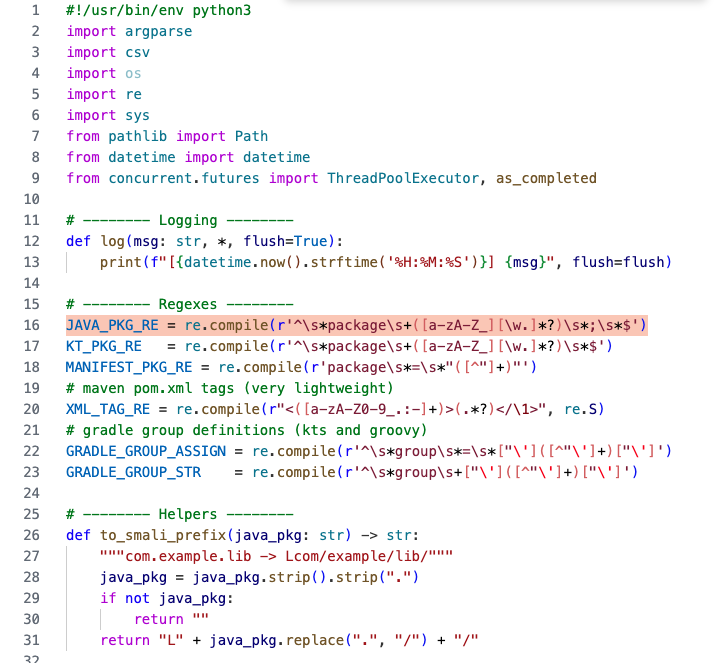
\includegraphics[width=0.5\textwidth,keepaspectratio]{image/Screenshot-make-fingerprints.png}
    \caption{The regular expressions to capture fingerprints in varius languages such as Java (code in python)}
    \label{fig:screenshot-make-fingerprints}
\end{figure}

\begin{figure}[htbp]
    \centering
    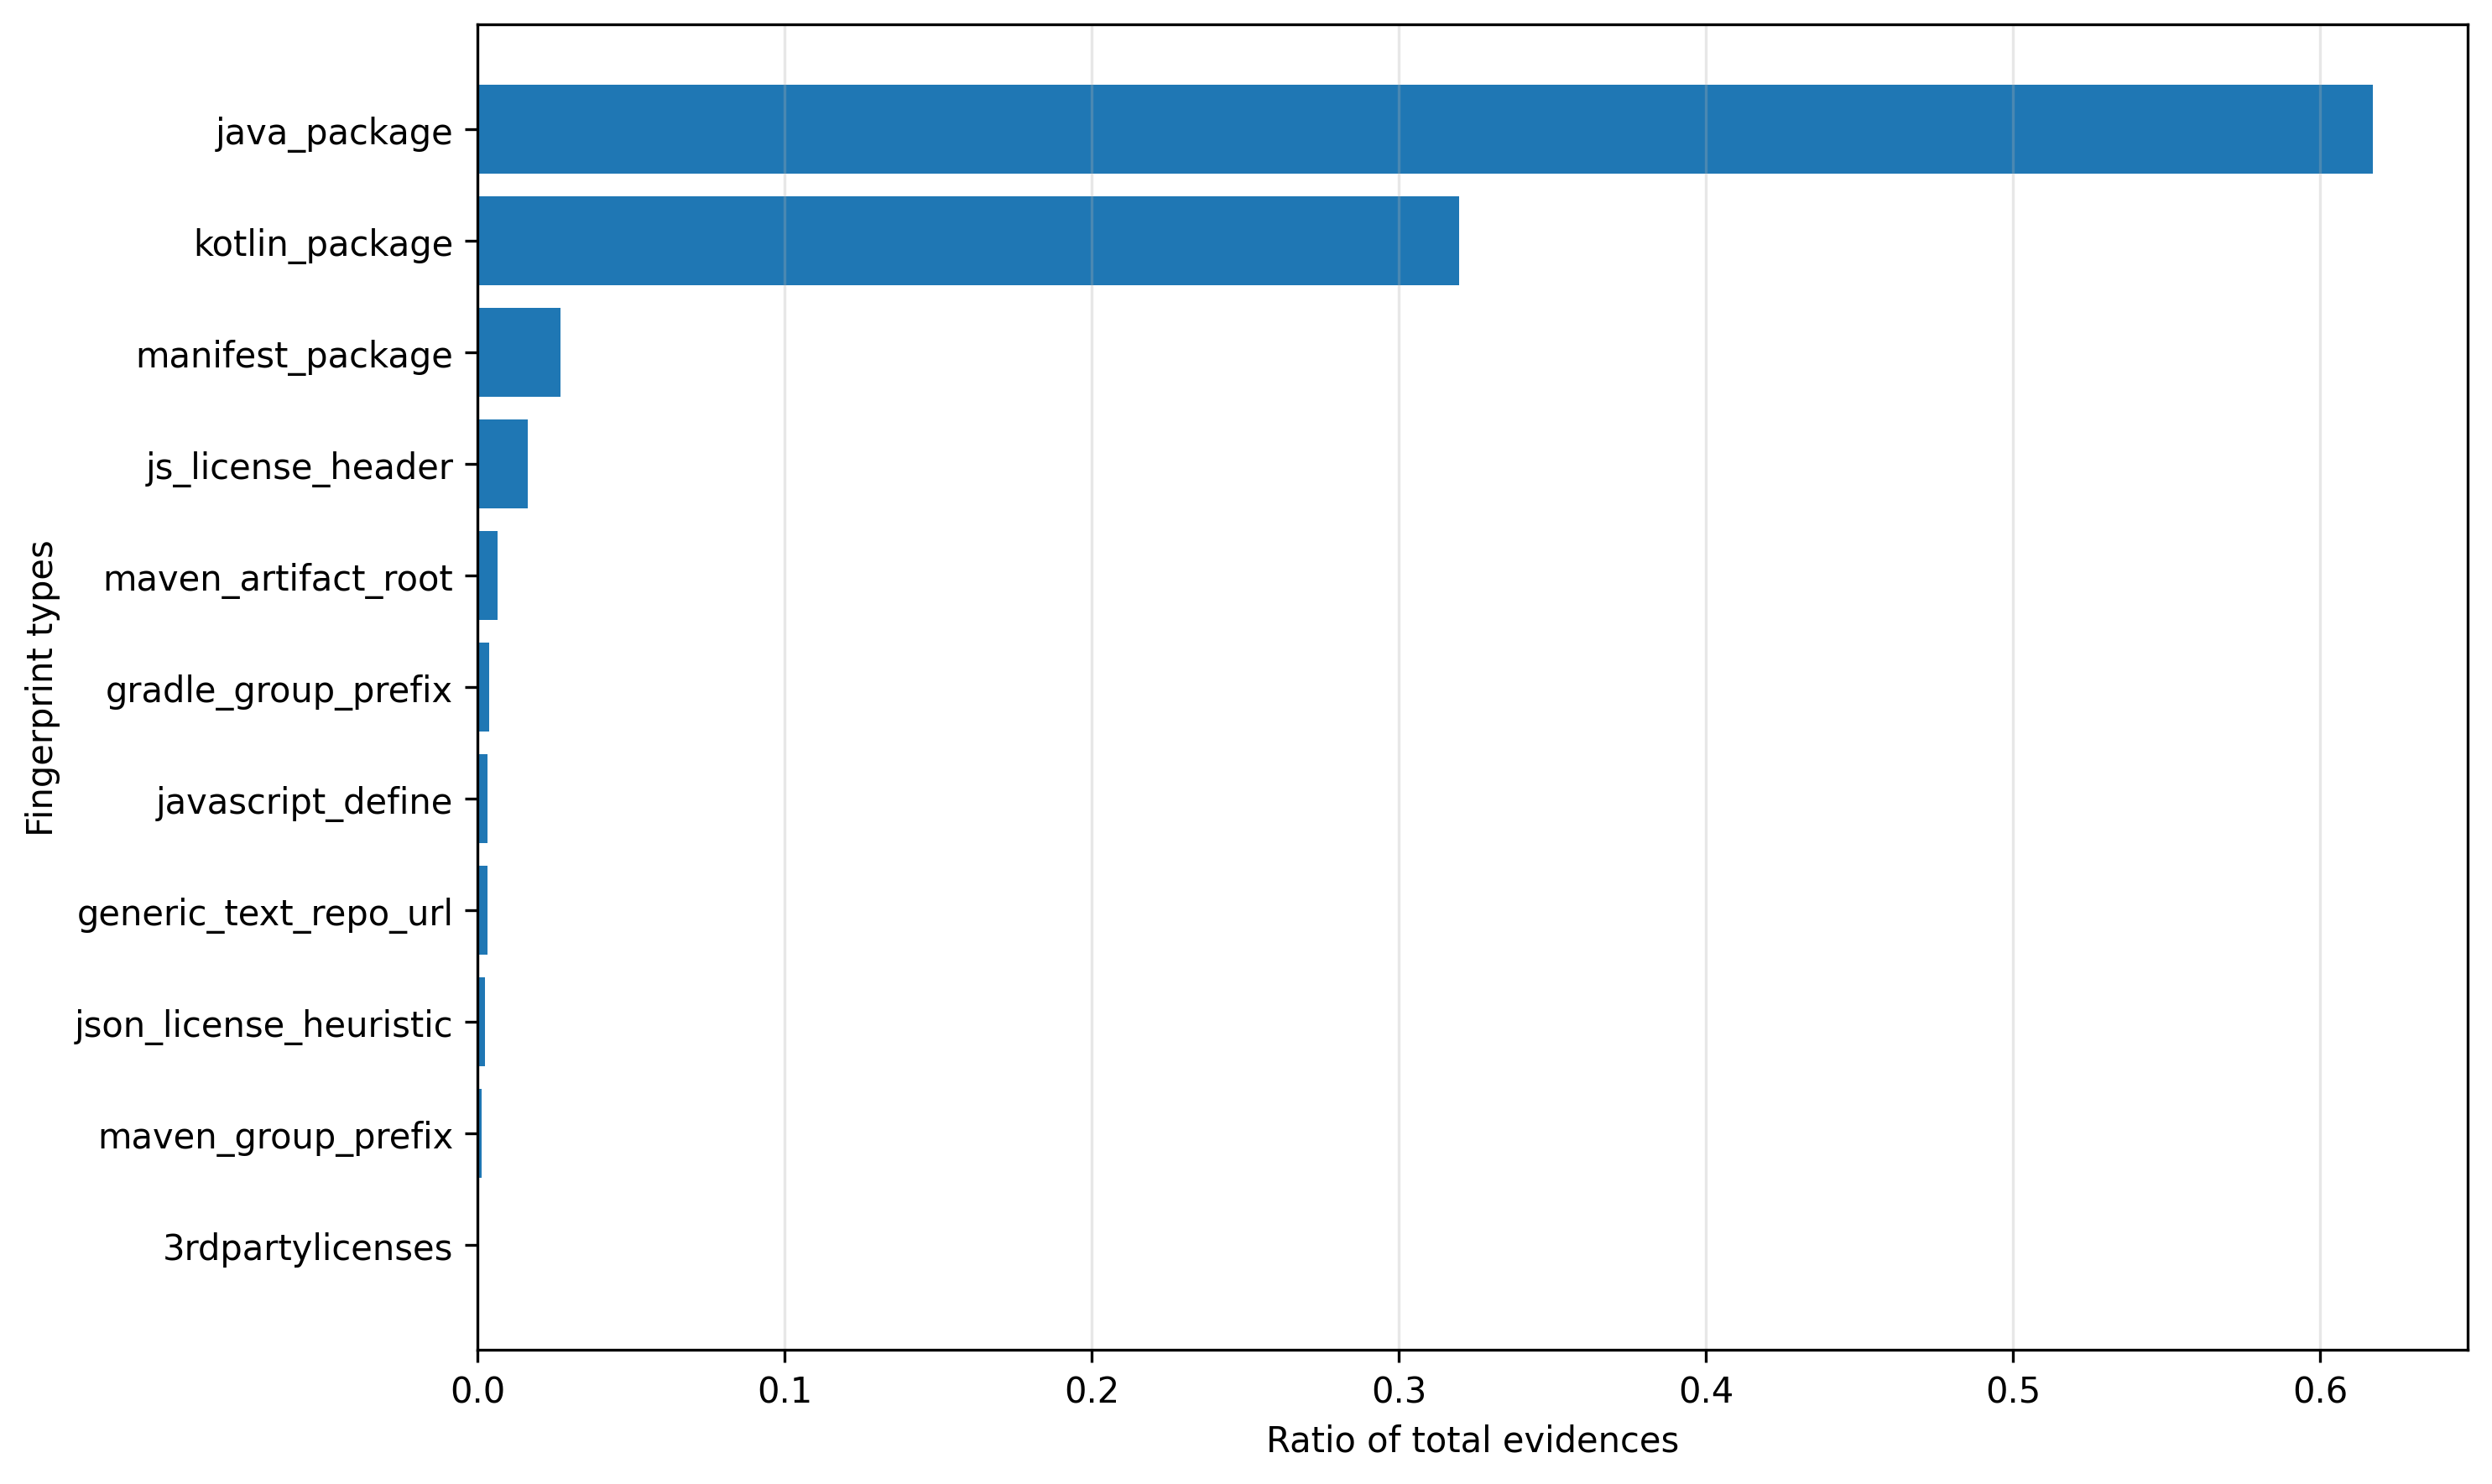
\includegraphics[width=0.8\textwidth,keepaspectratio]{image/fingerprint_type_ratio.png}
    \caption{Distribution of fingerprint types used to detect library evidence by application category in the final APK corpus}
    \label{fig:fingerprint-type-ratio}
\end{figure}

\begin{figure}[htbp]
    \centering
    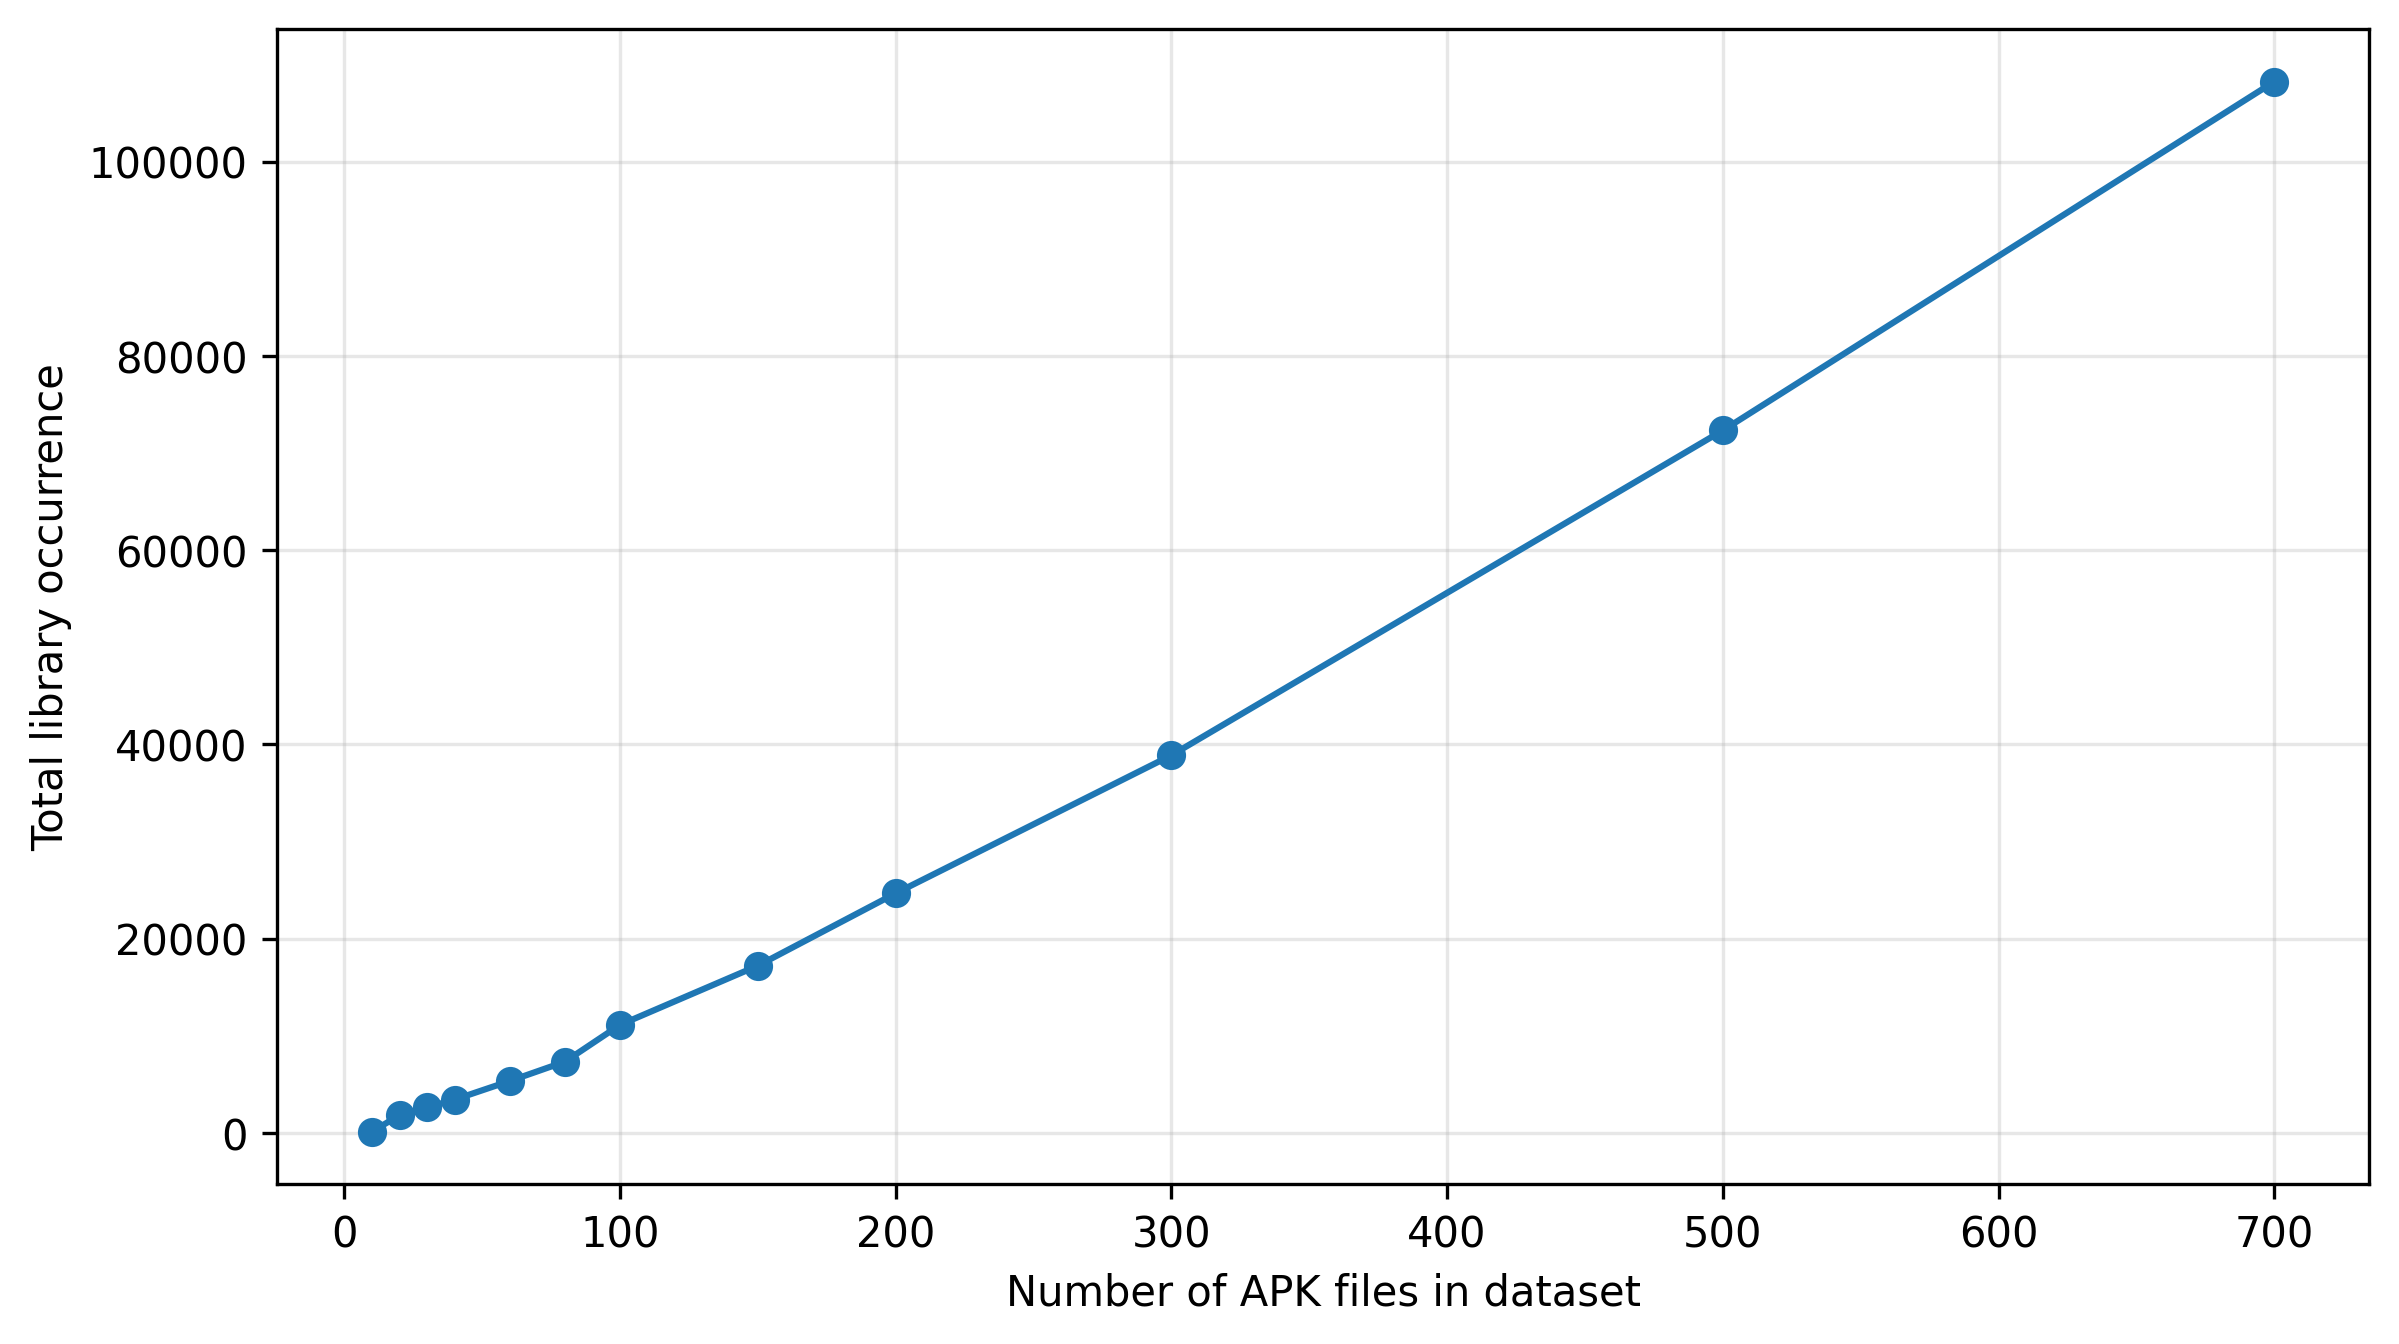
\includegraphics[width=\textwidth,keepaspectratio]{image/total_library_occurrences_by_apk_collection_size.png}
    \caption{Total detected library occurrences as the APK corpus size increases}
    \label{fig:total-libraries-occurrences}
\end{figure}

\begin{figure}[htbp]
    \centering
    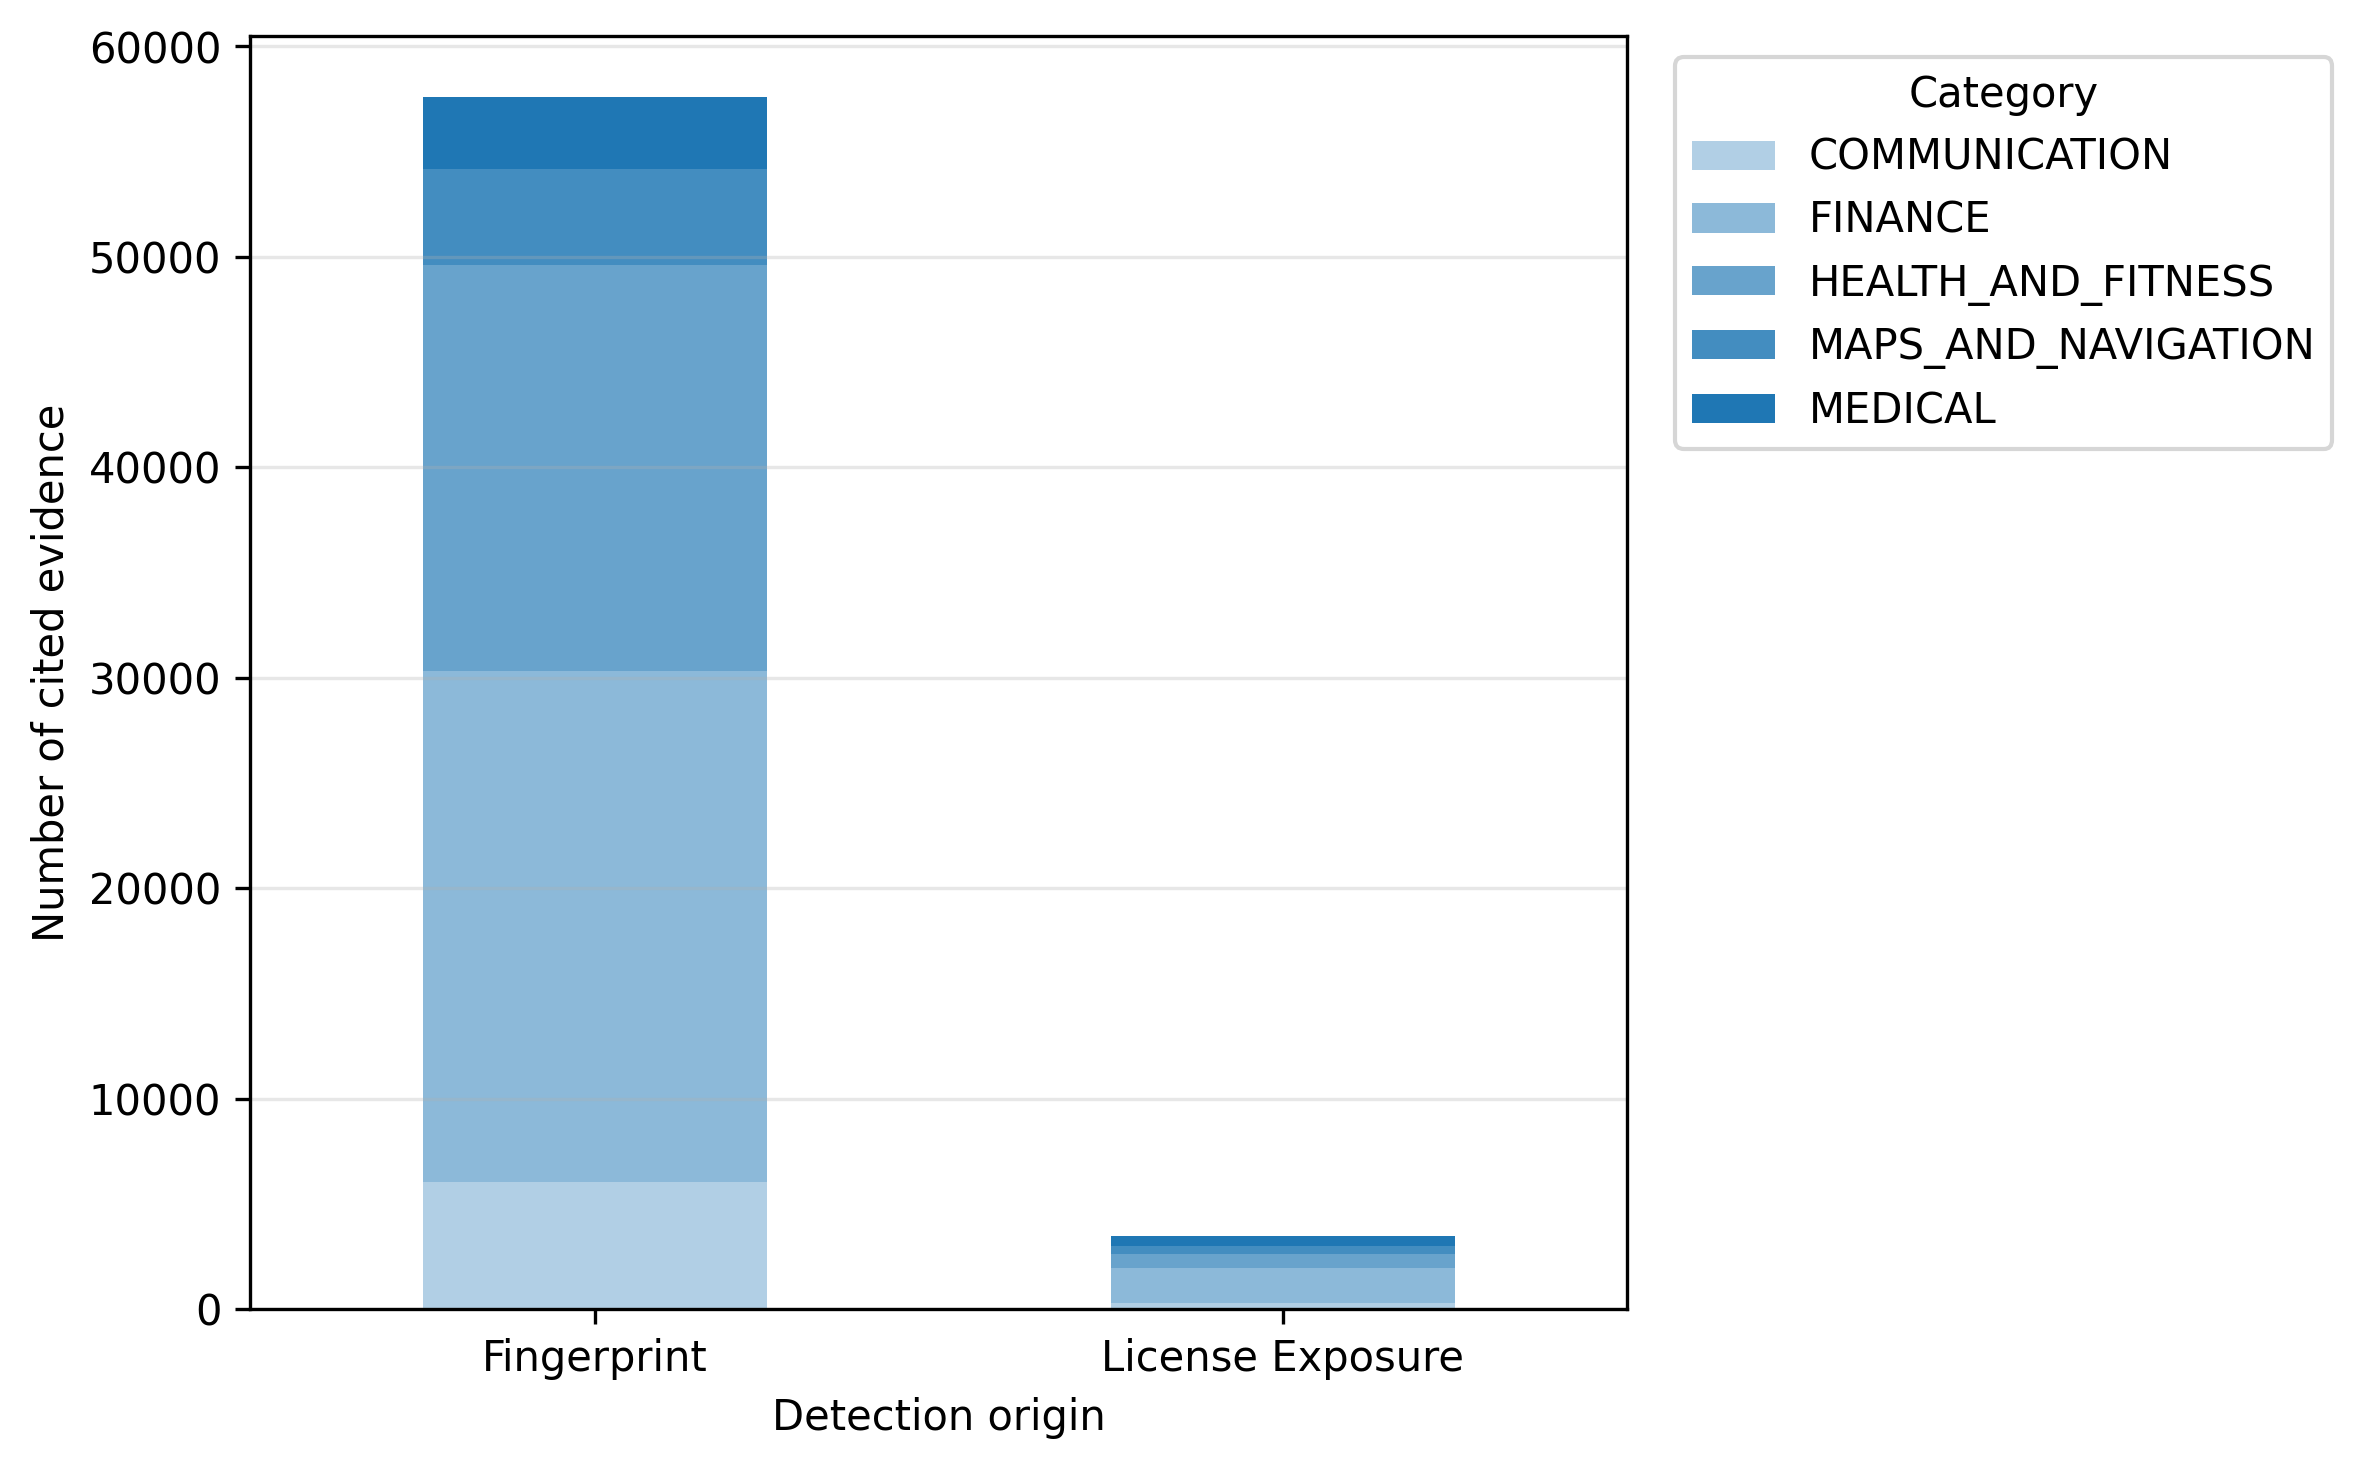
\includegraphics[width=\textwidth,keepaspectratio]{image/cited_rows_by_detection_origin_category.png}
    \caption{Detection origin of cited library records, comparing fingerprint evidence and license-exposure evidence by application category}
    \label{fig:fingerprints-vs-license-exposure-apk-700}
\end{figure}

\begin{figure}[htbp]
    \centering
    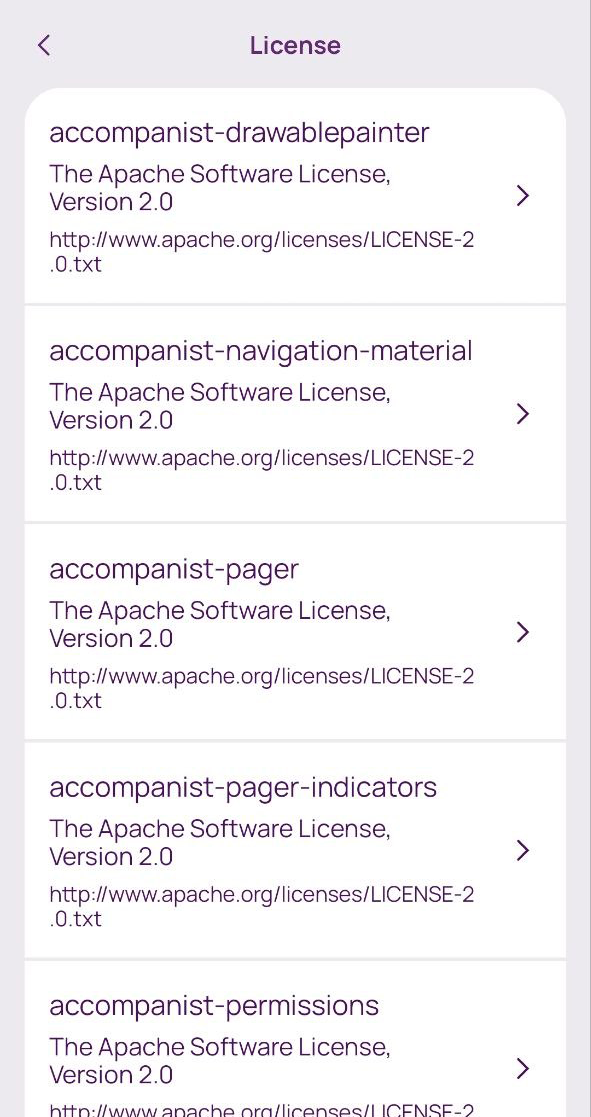
\includegraphics[width=0.5\textwidth,keepaspectratio]{image/budapestgo-licenses-frontend.png}
    \caption{BudapestGO in-app license screen generated through Sentry, a helper tool used in the CI/CD stack to audit runtime external libraries and export their licenses. Screenshot address: Menu, Information and help, License.}
    \label{fig:budapestgo-screenshot-licenses}
\end{figure}

\begin{figure}[htbp]
    \centering
    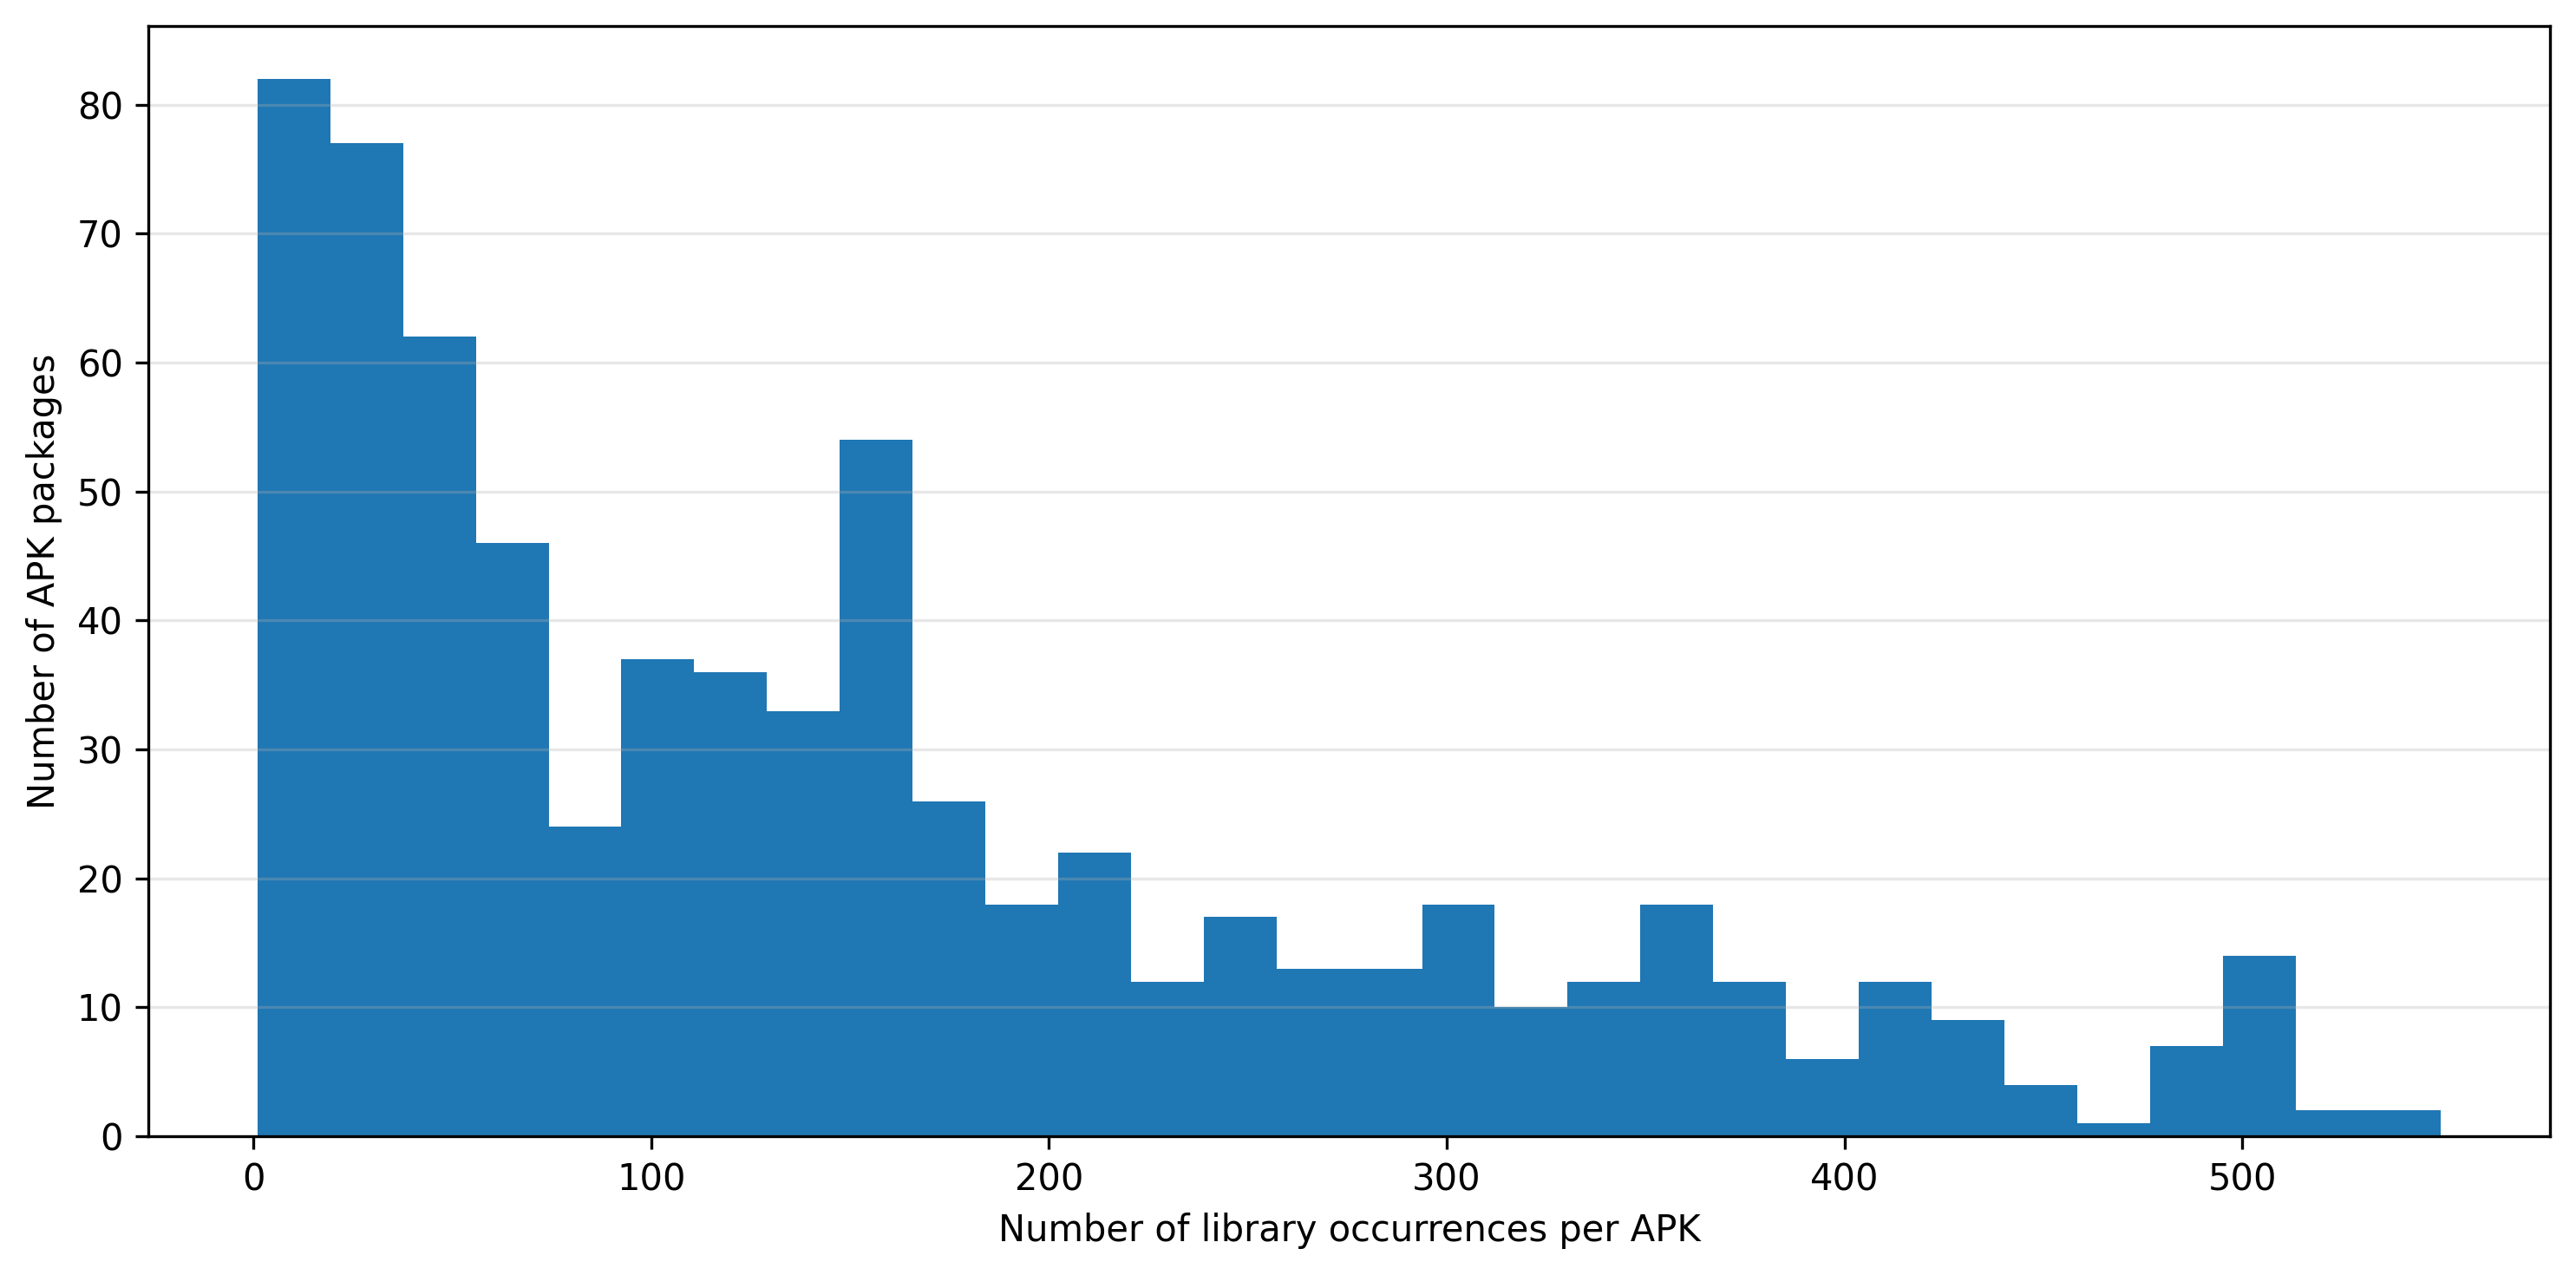
\includegraphics[width=\textwidth,keepaspectratio]{image/library_occurrences_per_apk_histogram.png}
    \caption{Histogram of detected library occurrences per APK in the final corpus}
    \label{fig:library-occurrences-per-apk-histogram}
\end{figure}

\begin{table}[htbp]
    \centering
    \caption[Summary report for the BudapestGO app]{Summary report for the BudapestGO app as a standalone APK added to the corpus}
    \label{tab:budapestgo-summary-report}
    \begin{tabular}{lr}
    \hline
    \textbf{Metric} & \textbf{Value} \\
    \hline
    Total library occurrences & 266 \\
    Total unique library occurrences & 91 \\
    Cited library occurrences & 255 \\
    Uncited library occurrences & 11 \\
    Cited ratio & 95.86\% \\
    Uncited ratio & 4.35\% \\
    Library occurrences detected by fingerprint & 68 \\
    Library occurrences detected by license-exposure & 251 \\
    Library occurrences detected by fingerprint and license-exposure & 53 \\
    Cited Library occurrences found by fingerprints & 57 \\
    Medium health library occurrences & 0 \\
    \hline
    \end{tabular}
    \end{table}


\begin{table}[!ht]
    \centering
    \begin{tabular}{|l|l|l|}
    \hline
        \textbf{app\_name} & \textbf{downloads} & \textbf{category} \\ \hline
        NoiseFit: Health \& Fitness & 50M+ & HEALTH\_AND\_FITNESS \\ \hline
        Bobble AI Keyboard Memes, Gifs & 50M+ & COMMUNICATION \\ \hline
        GoPay: Transfer, Payment, QRIS & 50M+ & FINANCE \\ \hline
        Taxsee Driver & 10M+ & MAPS\_AND\_NAVIGATION \\ \hline
        BSI Mobile & 10M+ & FINANCE \\ \hline
        Dhan: Share Market Trading App & 10M+ & FINANCE \\ \hline
        MEXC: Buy Bitcoin BTC \& Crypto & 10M+ & FINANCE \\ \hline
        Taptap Send: Money Transfer & 10M+ & FINANCE \\ \hline
        Boost Visual Voicemail & 10M+ & COMMUNICATION \\ \hline
        Agribank Plus & 10M+ & FINANCE \\ \hline
        CoinMarketCap: Crypto Tracker & 10M+ & FINANCE \\ \hline
        CHECK24 Vergleiche & 10M+ & FINANCE \\ \hline
        Upstox Stocks IPO Mutual Funds & 10M+ & FINANCE \\ \hline
        Planet Fitness & 10M+ & HEALTH\_AND\_FITNESS \\ \hline
        Cashi & 10M+ & FINANCE \\ \hline
        ABA Mobile & 10M+ & FINANCE \\ \hline
        Luno: Buy Bitcoin \& Crypto & 10M+ & FINANCE \\ \hline
        Monzo - Mobile Banking & 10M+ & FINANCE \\ \hline
        T-money GO - Taxi, Express Intercity & 10M+ & MAPS\_AND\_NAVIGATION \\ \hline
        imo beta -video calls and chat & 100M+ & COMMUNICATION \\ \hline
        Yandex Maps and Navigator & 100M+ & MAPS\_AND\_NAVIGATION \\ \hline
        BudapestGO & 1M+ & MAPS\_AND\_NAVIGATION \\ \hline
        in.kontakt & 1K+ & COMMUNICATION \\ \hline
        Cabrillo Credit Union & 10K+ & FINANCE \\ \hline
        UK Credit Union & 10K+ & FINANCE \\ \hline
        BrightStar CU Mobile & 10K+ & FINANCE \\ \hline
        Apple Bank Mobile Banking & 100K+ & FINANCE \\ \hline
    \end{tabular}
    \caption{List of apps for manual license investigation.}
    \label{tab:list-apps-manual-validation}
\end{table}


\begin{table}[htbp]
\centering
\caption[Merged summary KPIs for the 699 APK corpus]{Merged summary KPIs for the 699 APK corpus; each dataset row represents one evidence instance AKA library occurrences}
\label{tab:summary-kpis-final-corpus}
\begin{tabular}{lr}
\hline
\textbf{Metric} & \textbf{Value} \\
\hline
Total library occurrences & 108,234 \\
Unique APK packages & 699 \\
Library occurrences with missing repository URL & 0 \\
Total generated fingerprints & 6,536 \\
Cited library occurrences & 59,954 \\
Uncited library occurrences & 48,280 \\
Cited ratio of total library occurrences & 55.39\% \\
Uncited ratio of total library occurrences & 44.61\% \\
Library occurrences detected by fingerprint evidence & 105,874 \\
Library occurrences detected by license-exposure evidence & 3,478 \\
Cited library occurrences found by fingerprints & 57,594 \\
Fingerprint ratio among cited library occurrences & 96.06\% \\
License-exposure ratio among cited library occurrences & 5.80\% \\
Average library occurrences per APK & 154.84 \\
Median library occurrences per APK & 123 \\
Minimum library occurrences per APK & 1 \\
Maximum library occurrences per APK & 550 \\
Unique repository URLs & 636\textsuperscript{*} \\
Unique cloned GitHub repository attempts & 274\textsuperscript{*} \\
GitHub repositories found & 220 \\
GitHub repositories not found or returned error & 54 \\
\hline
\end{tabular}

{\footnotesize\textit{Note.} The number of unique repository URLs is higher than the number of cloned GitHub repository attempts because some repositories contain more than one library, and some license URLs point to a specific library or subdirectory inside a repository rather than to a separate repository.}
\end{table}
\end{document}